\begin{figure}[ht!]
     \centering
     \begin{subfigure}[b]{\textwidth}
         \centering
         \caption{Partial dependence plot (SHAP) for Estonia}
         \label{fig:5b_EST}
         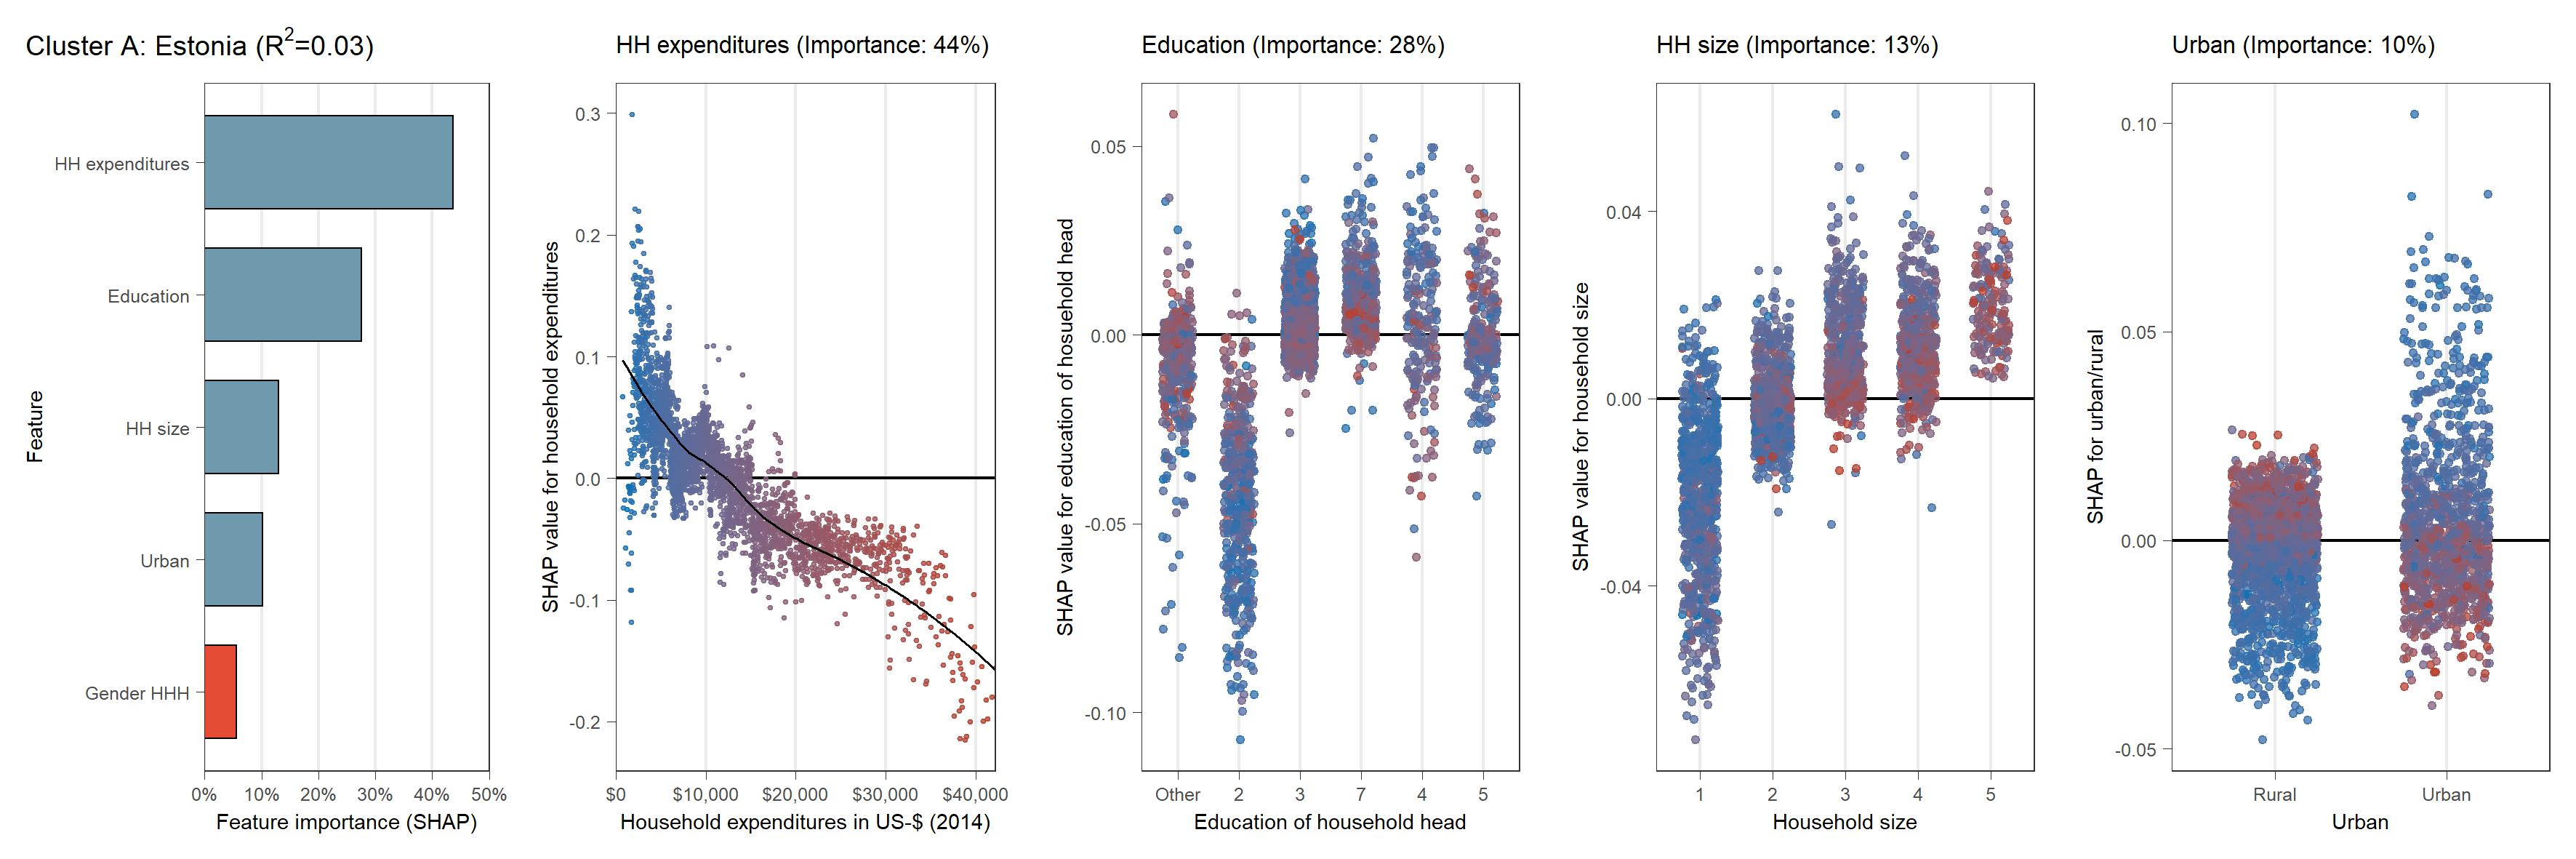
\includegraphics[width=\textwidth]{Figure_5b_EST}      
     \end{subfigure}
    \\
    \vspace{0.5cm}
     \begin{subfigure}[b]{\textwidth}
         \centering
         \caption{Partial dependence plot (SHAP) for Bulgaria}
         \label{fig:5b_BGR}
         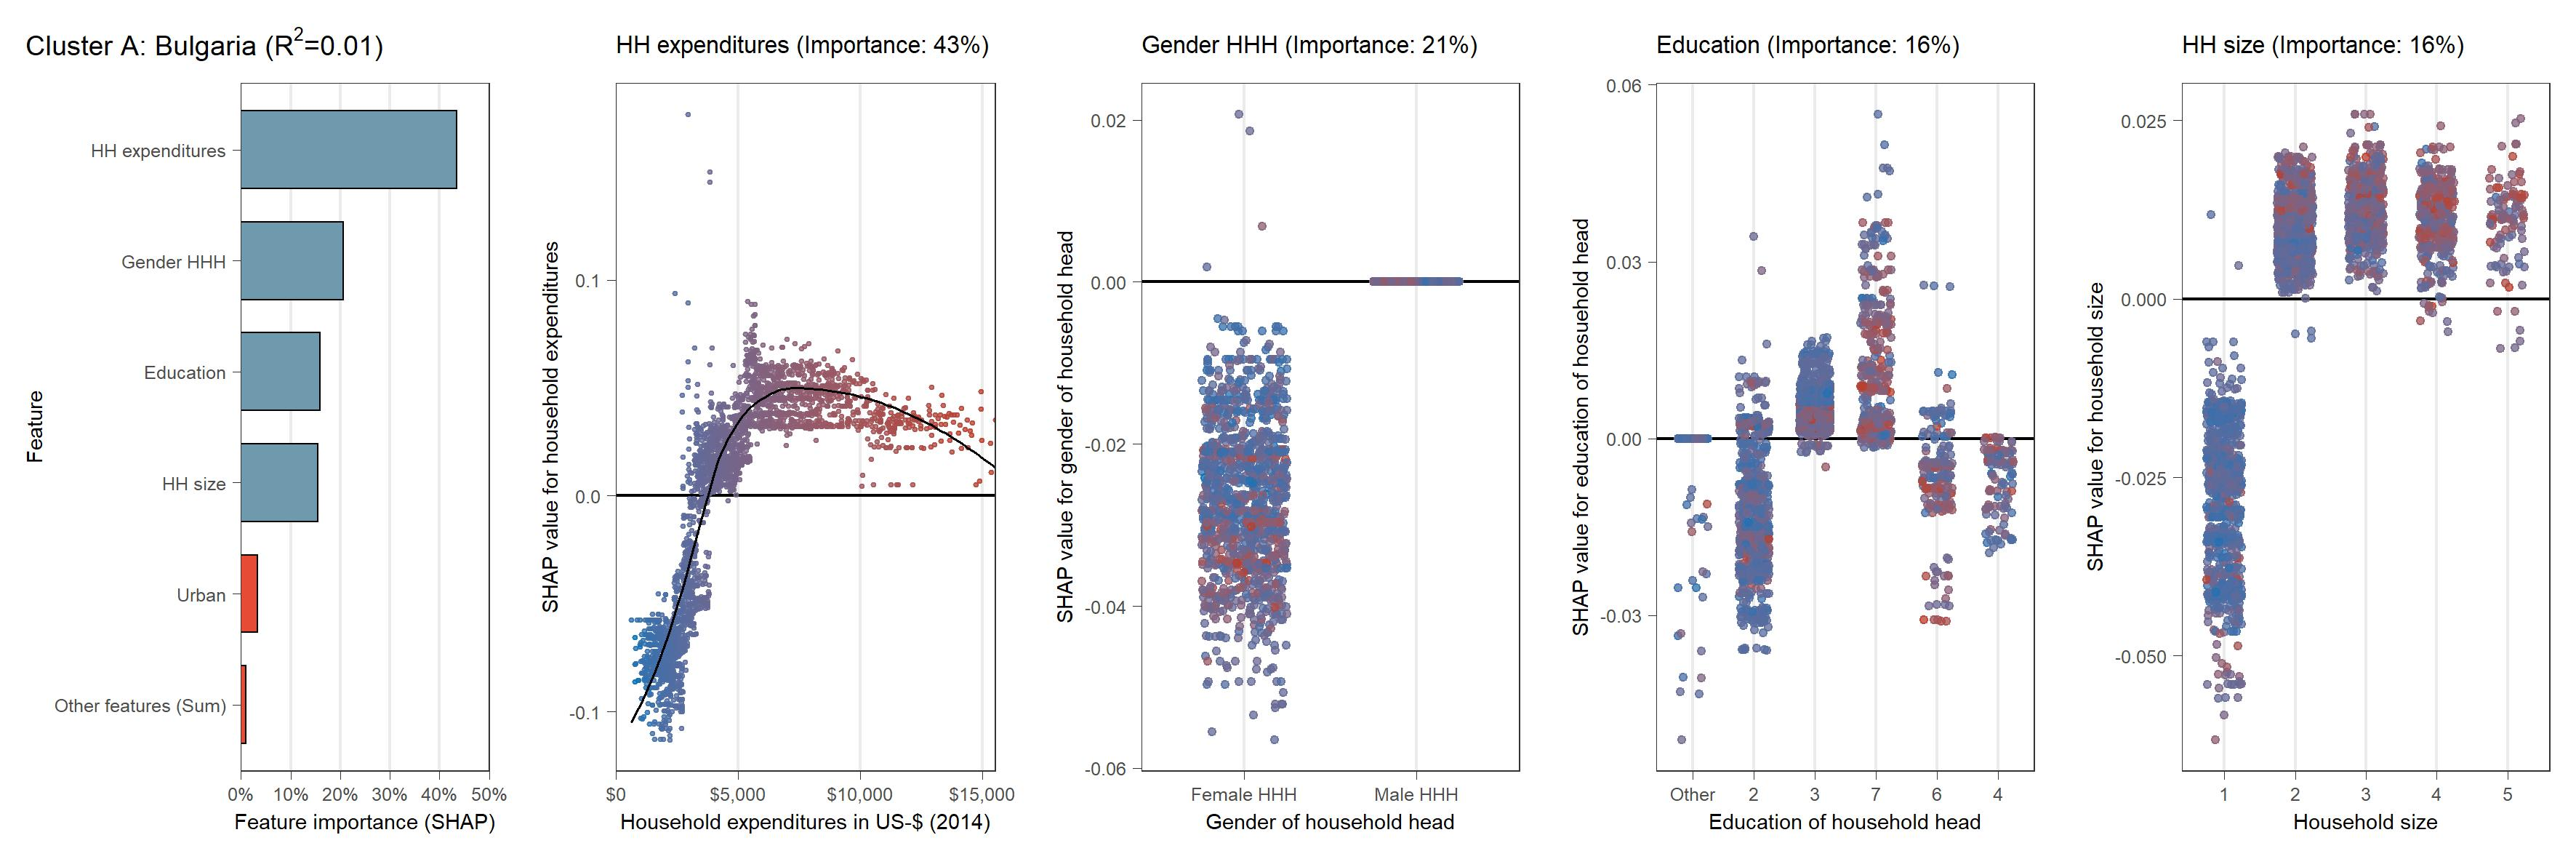
\includegraphics[width=\textwidth]{Figure_5b_BGR}
     \end{subfigure}
    \\
    \vspace{0.5cm}
     \begin{subfigure}[b]{1\textwidth}
         \centering
         \caption{Partial dependence plot (SHAP) for Hungary}
         \label{fig:5b_HUN}
         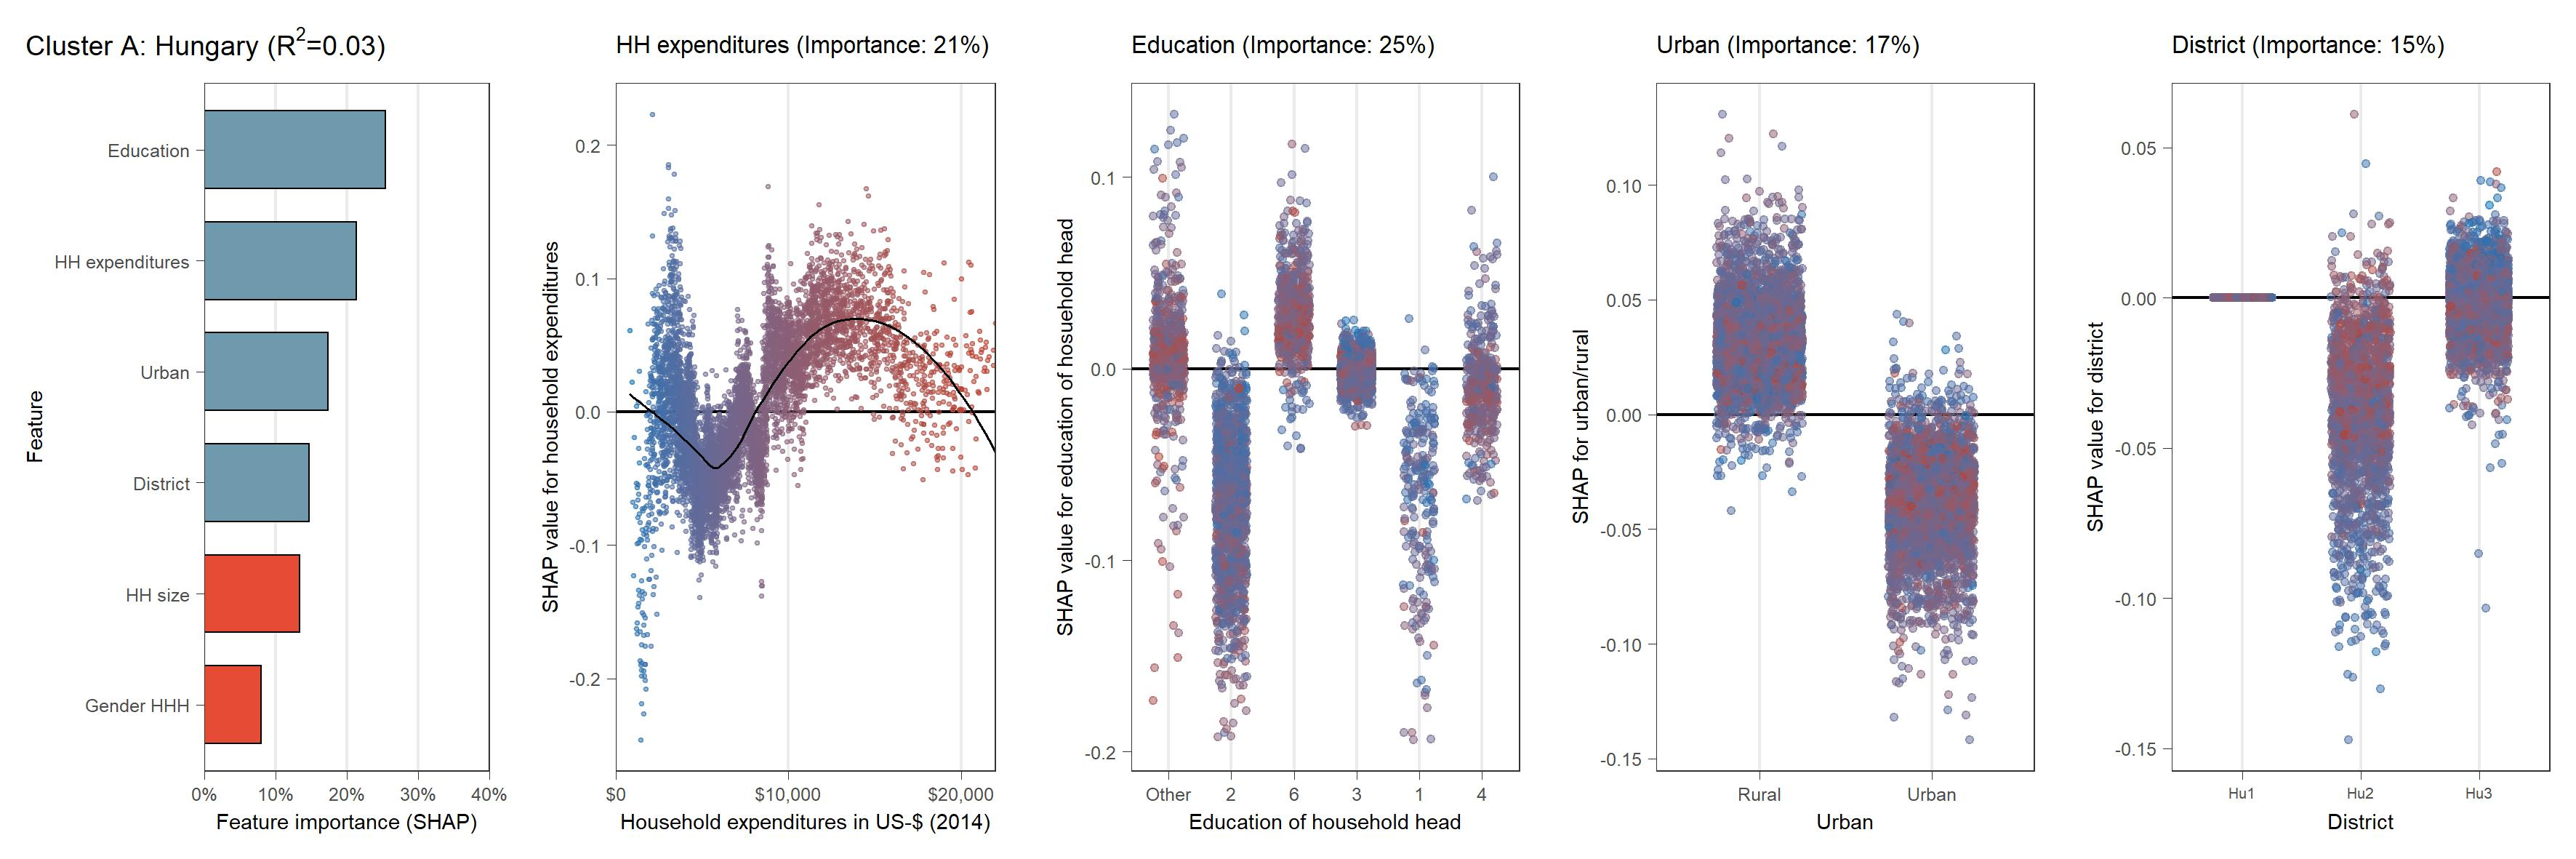
\includegraphics[width=\textwidth]{Figure_5b_HUN}
     \end{subfigure}
     \\
     \vspace{0.5cm}
        \begin{subcaption2}
     This figure shows SHAP-values for predicting carbon intensity over feature values for 87 countries in order of nine country-clusters. The bar chart displays normalized average absolute SHAP-values for all features. Features with less than 3\% of normalized SHAP-values are subsumed as "Other features (Sum)". Charts show SHAP-values over total household expenditures for all countries and for the three most important features in each country besides total household expenditures. Colors represent household expenditures with blue (red) colors indicating lower (higher) household expenditures.
     \end{subcaption2}
     \end{figure}
     
\begin{figure}[ht!]\ContinuedFloat
    \centering
   \begin{subfigure}[b]{\textwidth}
         \centering
         \caption{Partial dependence plot (SHAP) for Suriname}
         \label{fig:5b_SUR}
         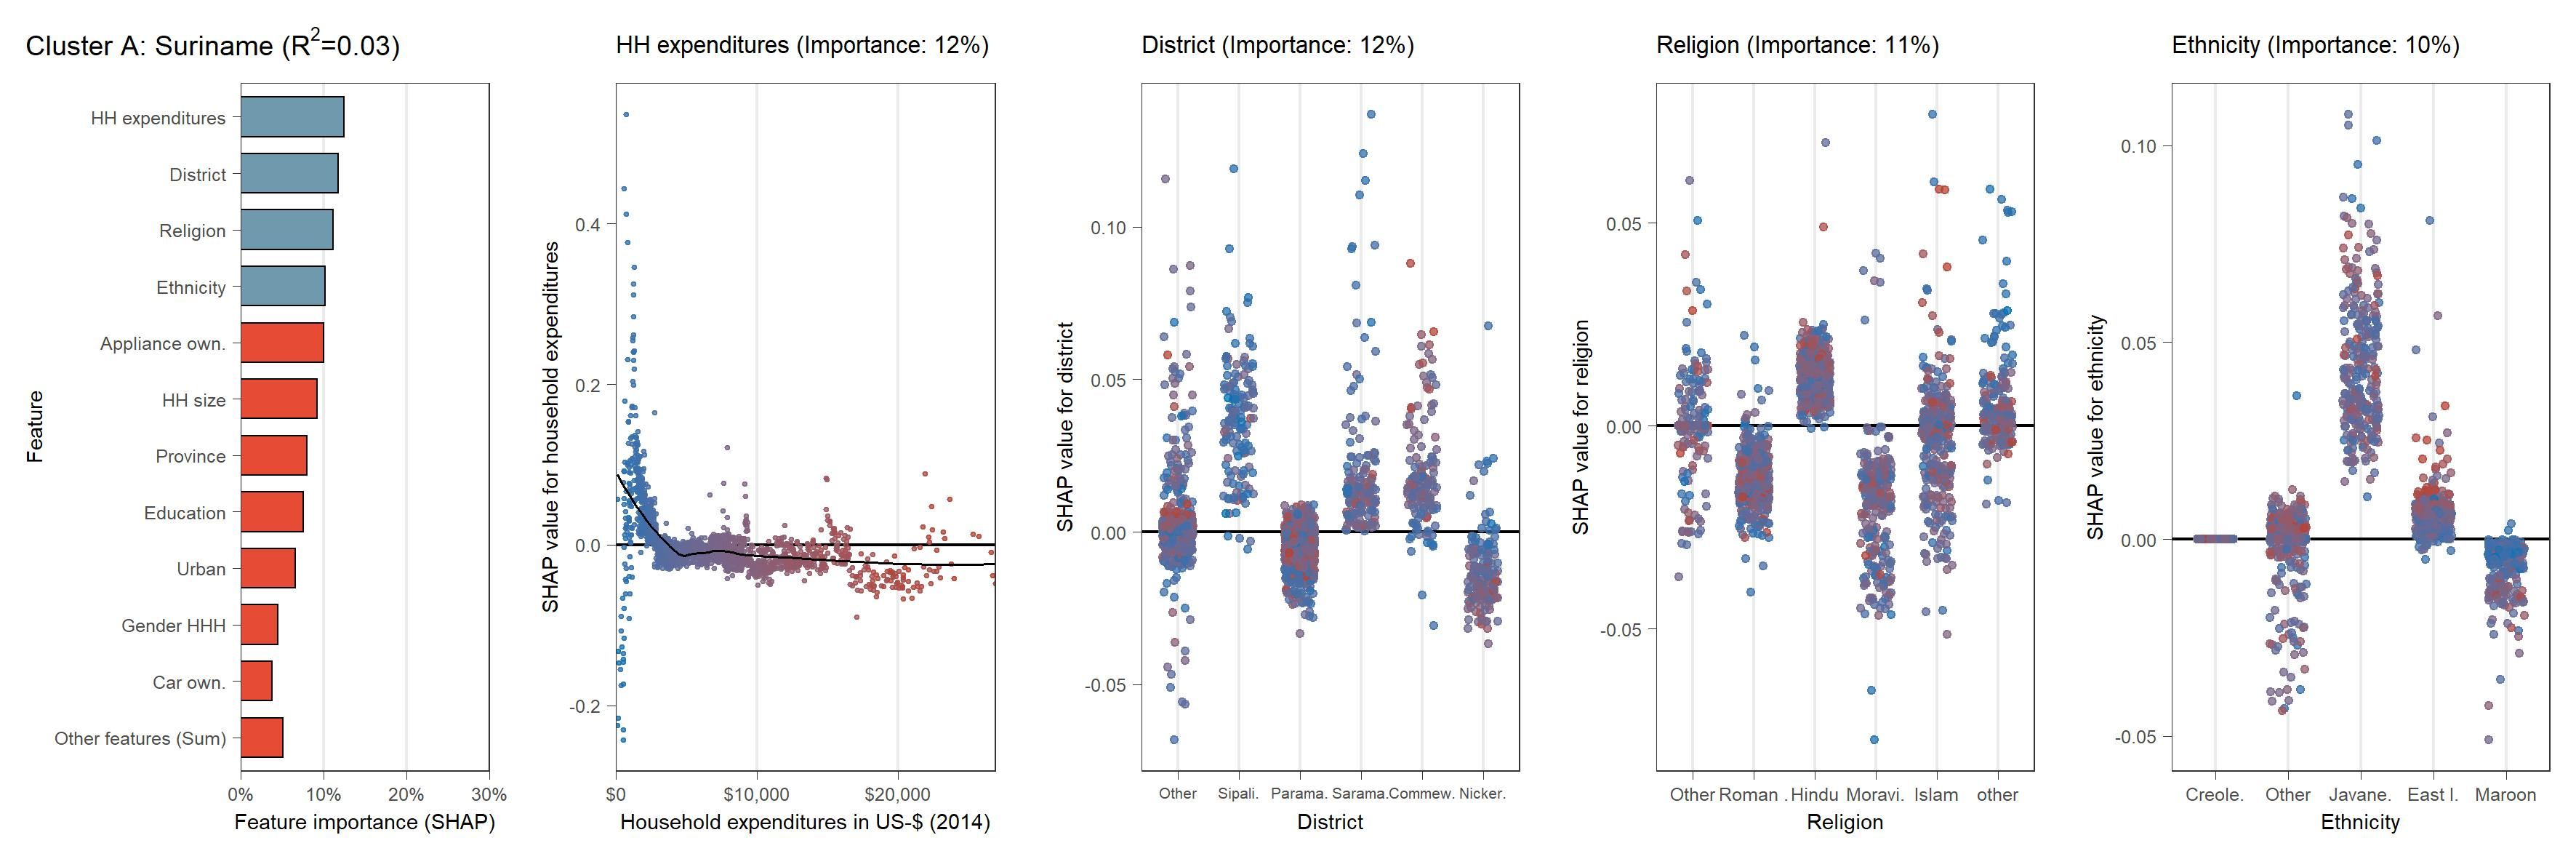
\includegraphics[width=\textwidth]{Figure_5b_SUR}         
     \end{subfigure}
    \\
    \vspace{0.5cm}
   \begin{subfigure}[b]{\textwidth}
         \centering
         \caption{Partial dependence plot (SHAP) for Morocco}
         \label{fig:5b_MAR}
         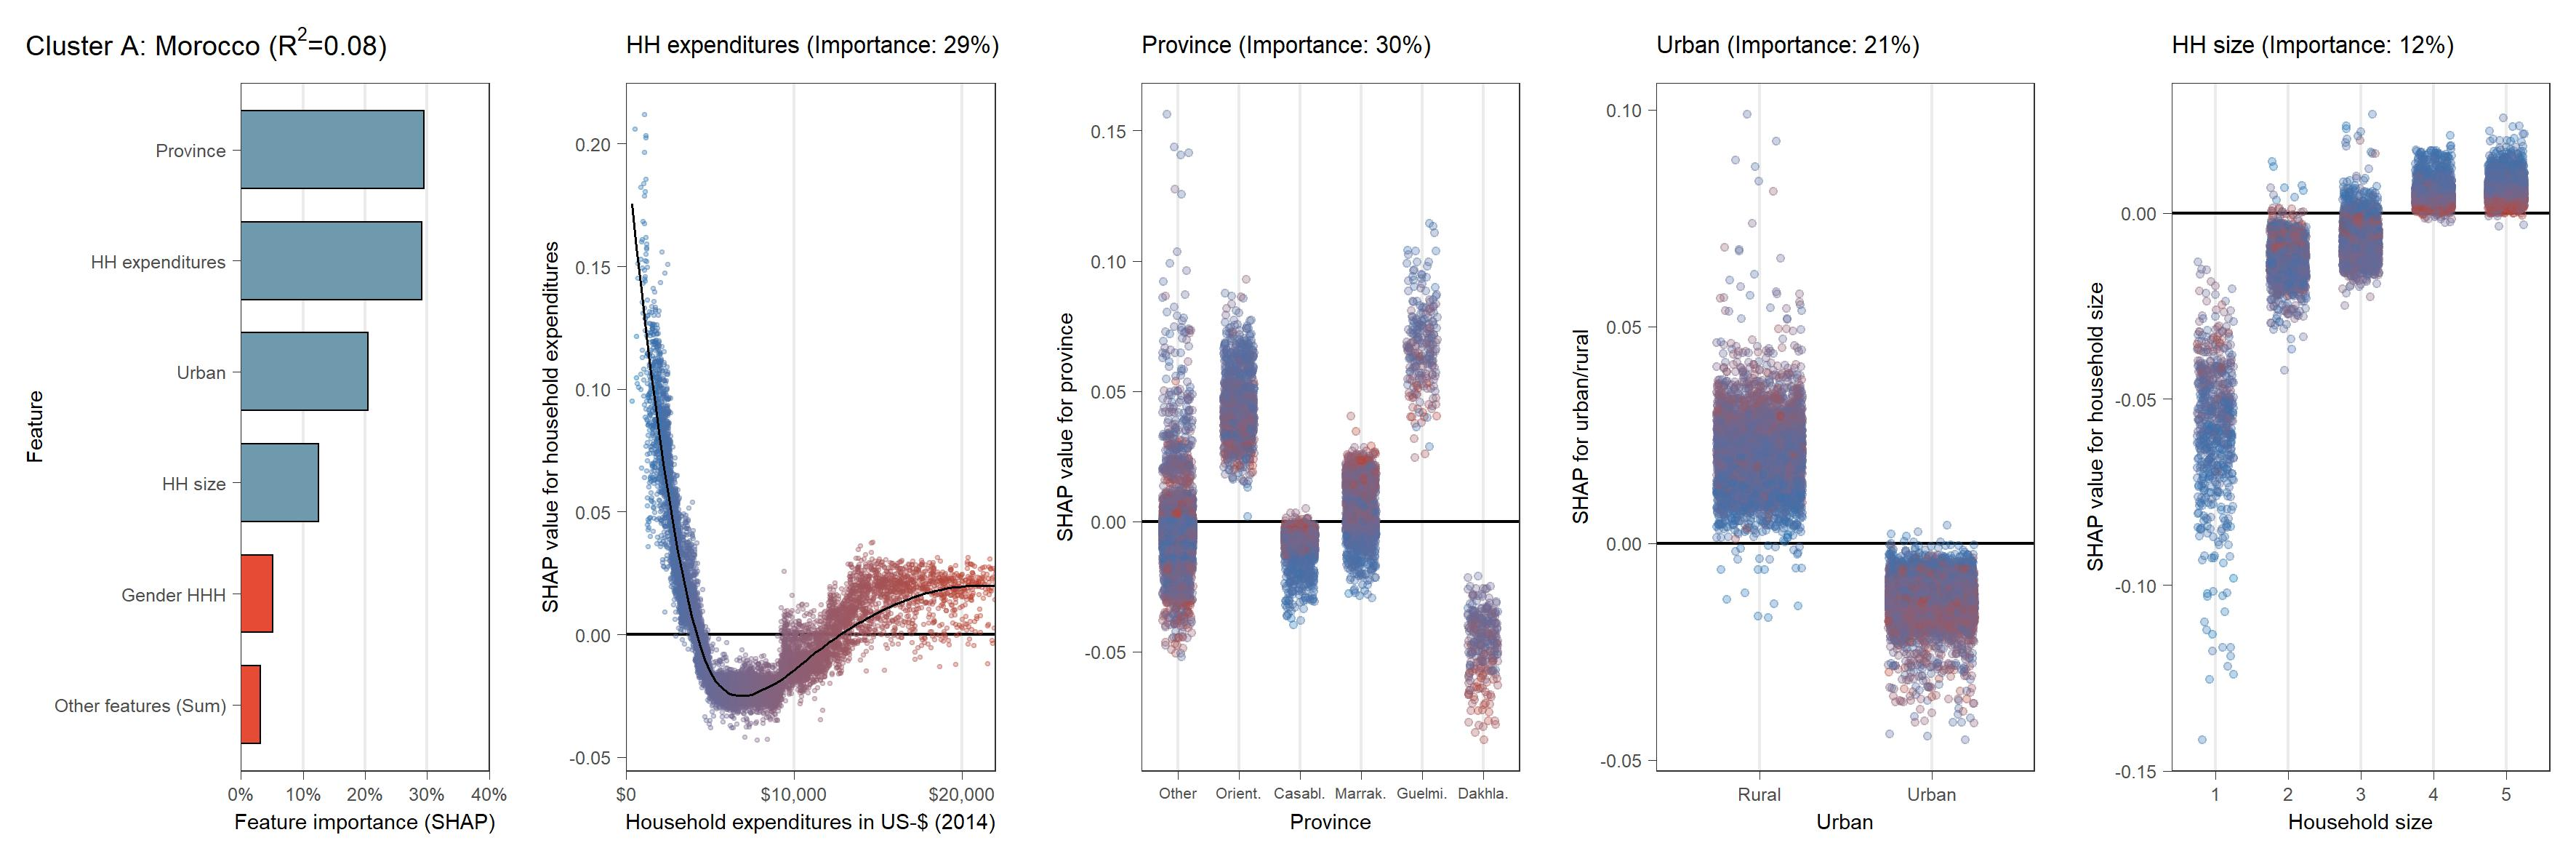
\includegraphics[width=\textwidth]{Figure_5b_MAR}         
     \end{subfigure}
    \\
    \vspace{0.5cm}
   \begin{subfigure}[b]{\textwidth}
         \centering
         \caption{Partial dependence plot (SHAP) for Greece}
         \label{fig:5b_GRC}
         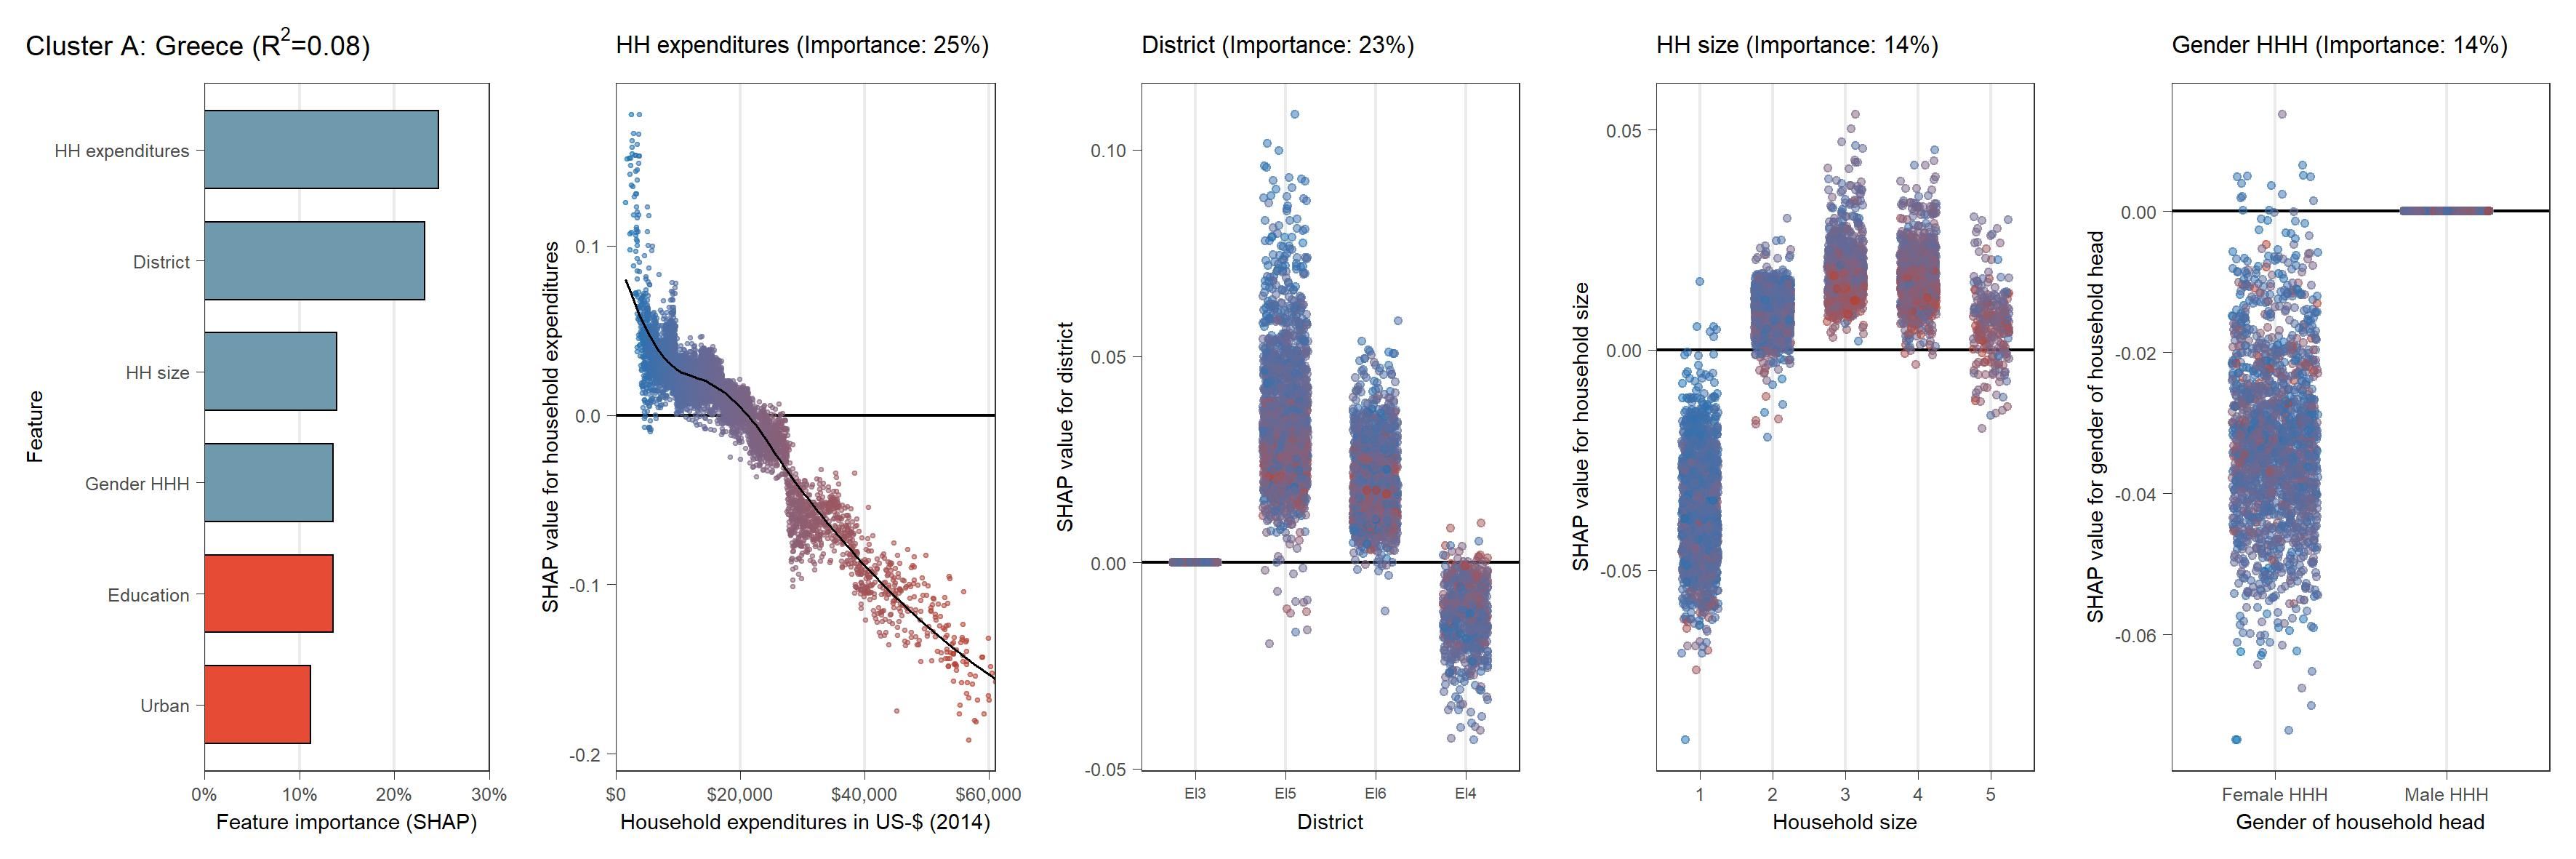
\includegraphics[width=\textwidth]{Figure_5b_GRC}
    \end{subfigure}
    \\
    \vspace{0.5cm}
    \begin{subcaption2}
     This figure shows SHAP-values for predicting carbon intensity over feature values for 87 countries in order of nine country-clusters. The bar chart displays normalized average absolute SHAP-values for all features. Features with less than 3\% of normalized SHAP-values are subsumed as "Other features (Sum)". Charts show SHAP-values over total household expenditures for all countries and for the three most important features in each country besides total household expenditures. Colors represent household expenditures with blue (red) colors indicating lower (higher) household expenditures.
     \end{subcaption2}
\end{figure}

\begin{figure}[ht!]\ContinuedFloat
    \centering
   \begin{subfigure}[b]{\textwidth}
         \centering
         \caption{Partial dependence plot (SHAP) for Sweden}
         \label{fig:5b_SWE}
         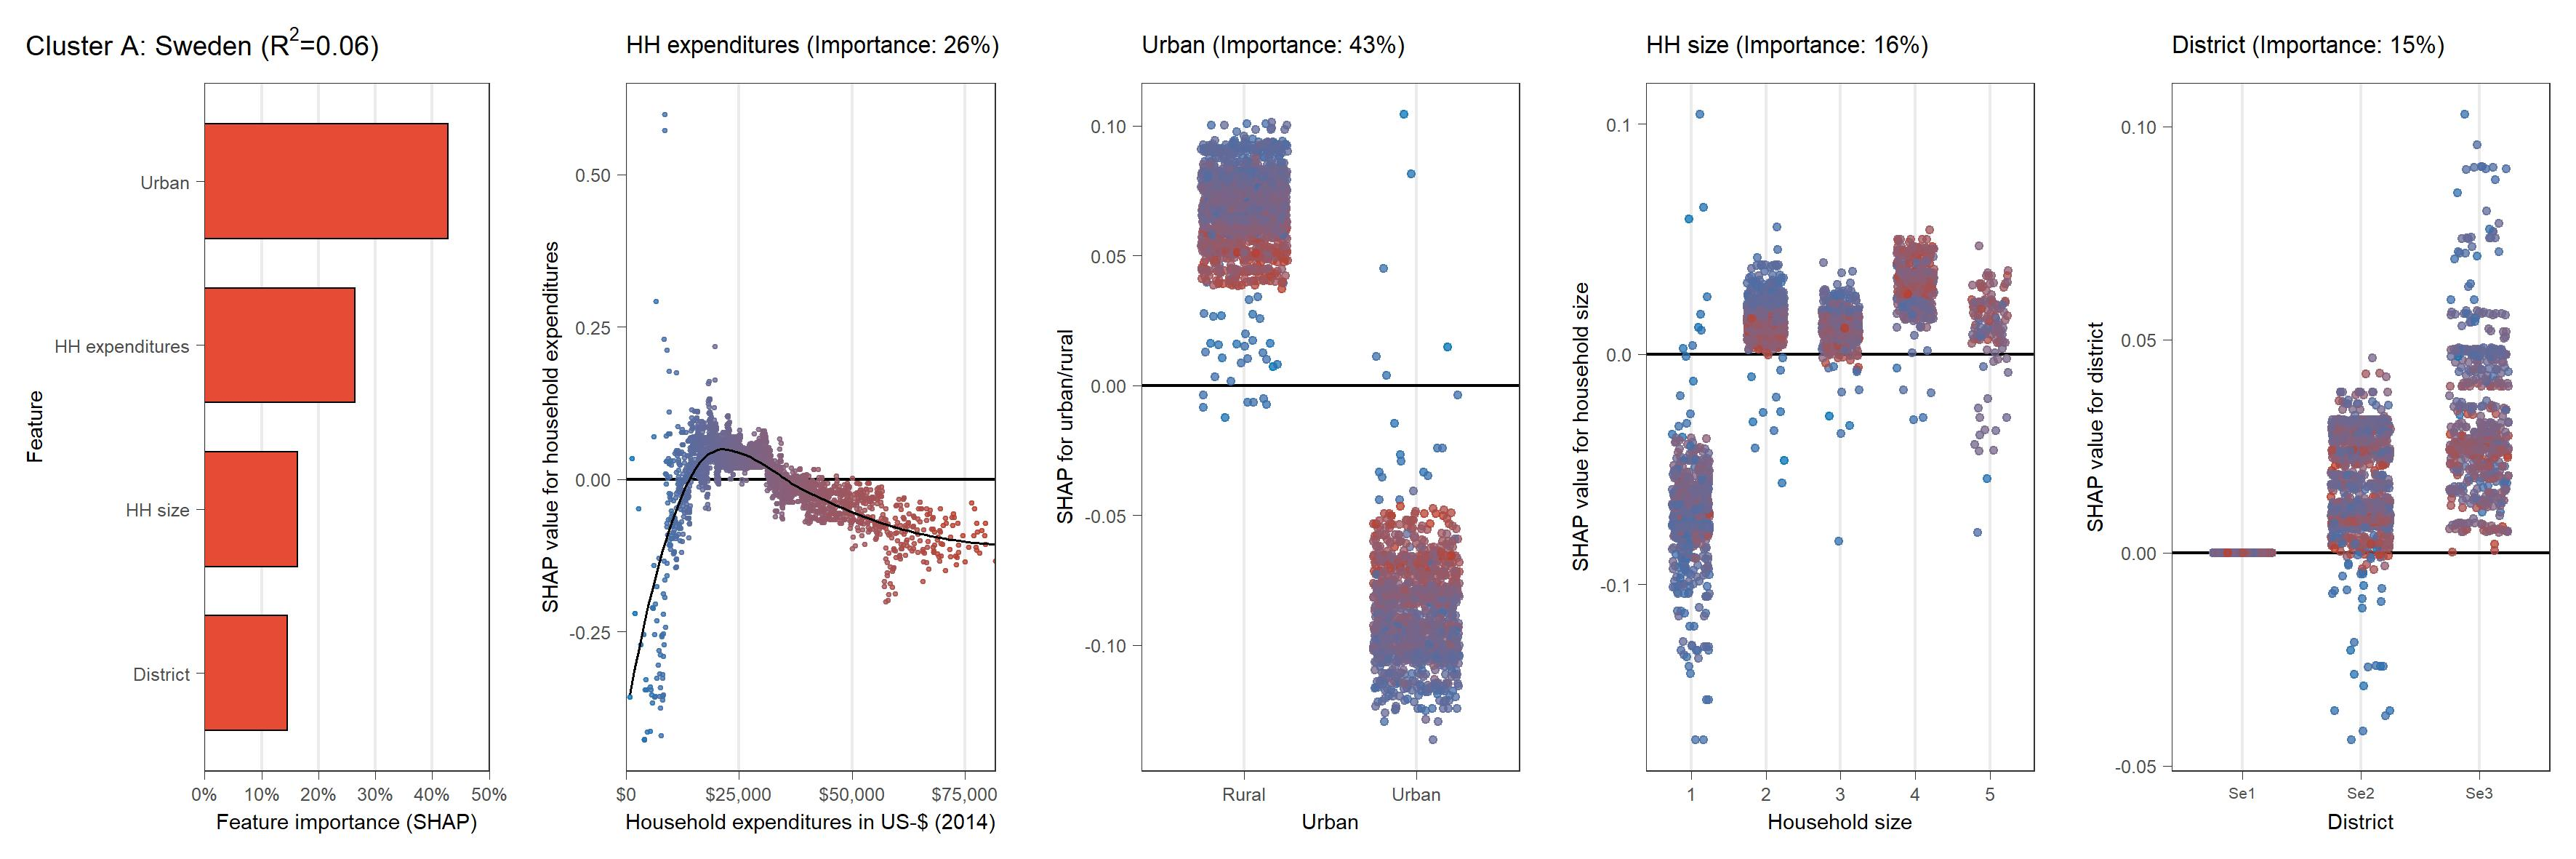
\includegraphics[width=\textwidth]{Figure_5b_SWE}         
     \end{subfigure}
    \\
    \vspace{0.5cm}
   \begin{subfigure}[b]{\textwidth}
         \centering
         \caption{Partial dependence plot (SHAP) for Serbia}
         \label{fig:5b_SRB}
         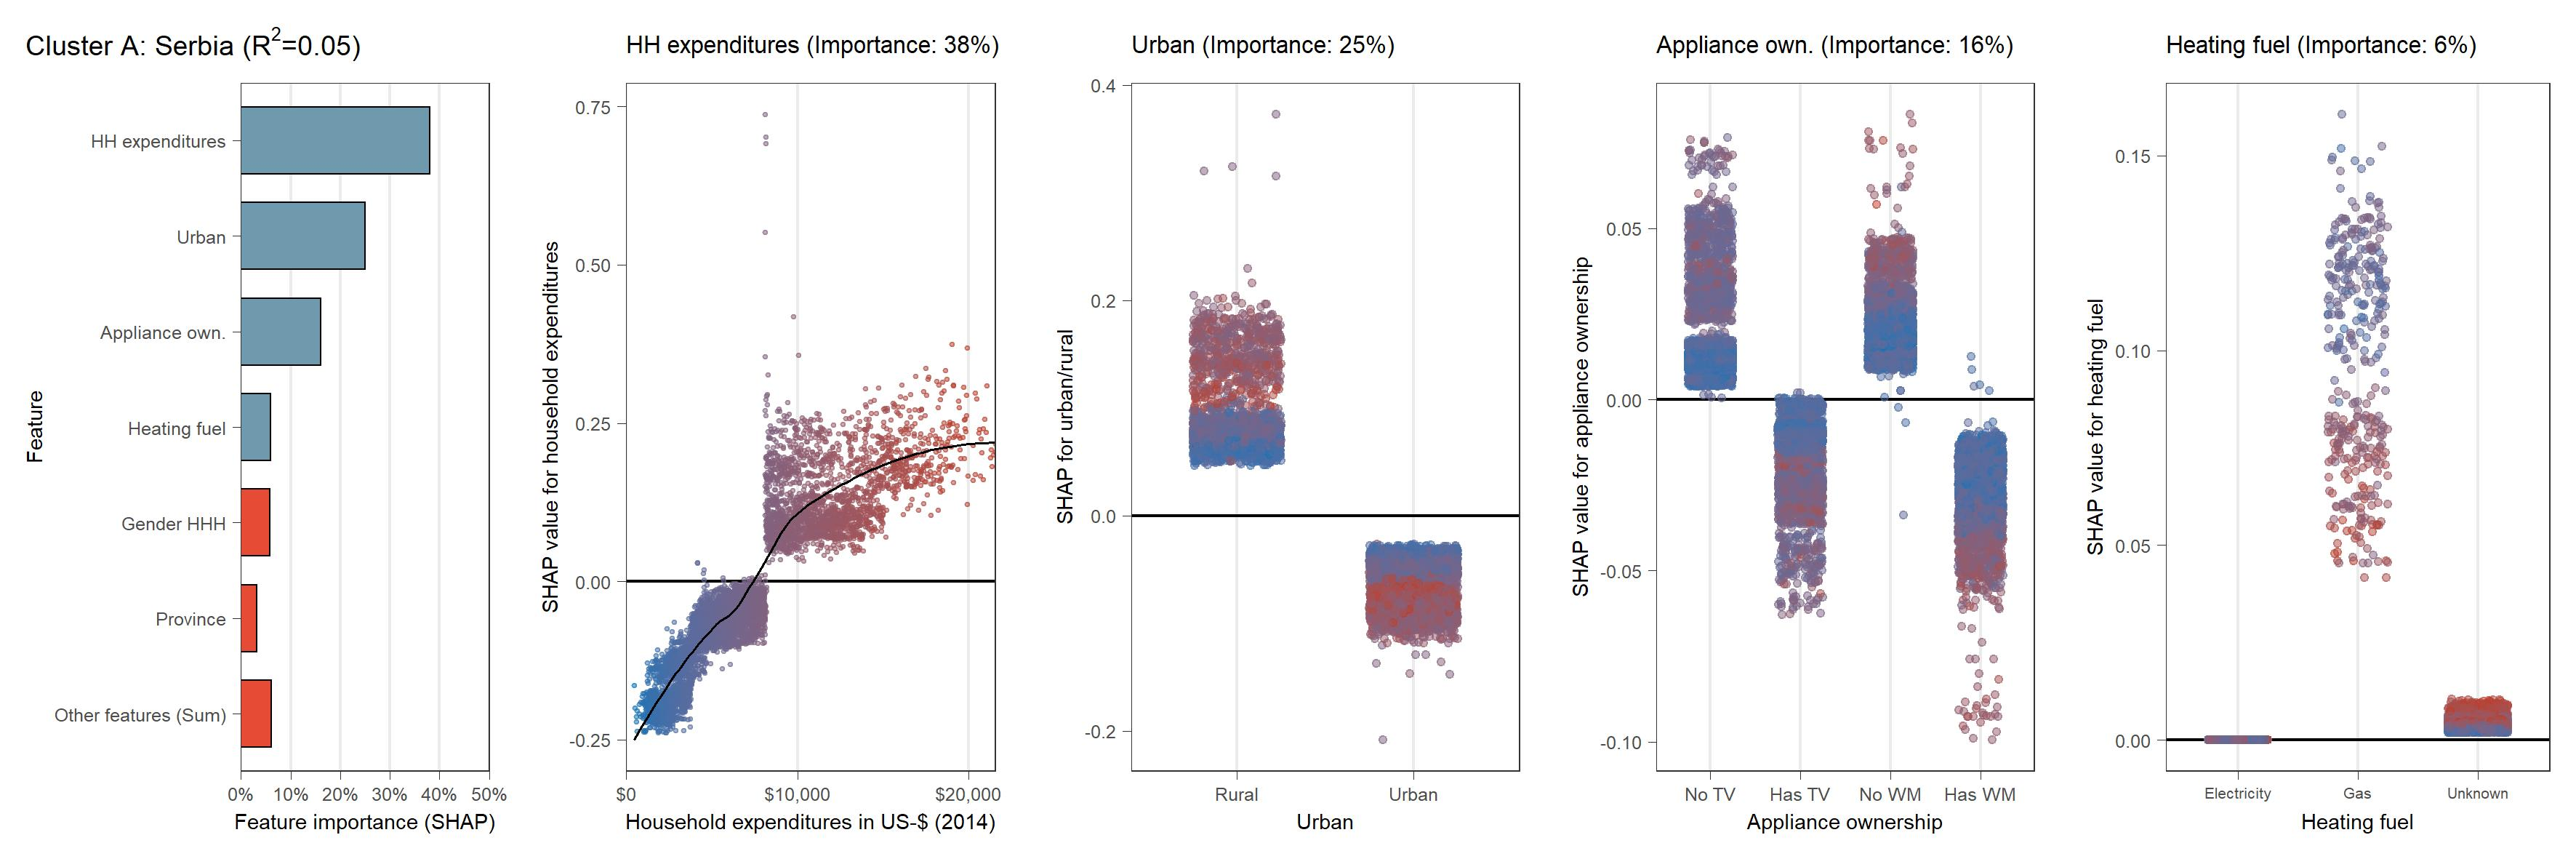
\includegraphics[width=\textwidth]{Figure_5b_SRB}         
     \end{subfigure}
    \\
    \vspace{0.5cm}
   \begin{subfigure}[b]{\textwidth}
         \centering
         \caption{Partial dependence plot (SHAP) for Croatia}
         \label{fig:5b_HRV}
         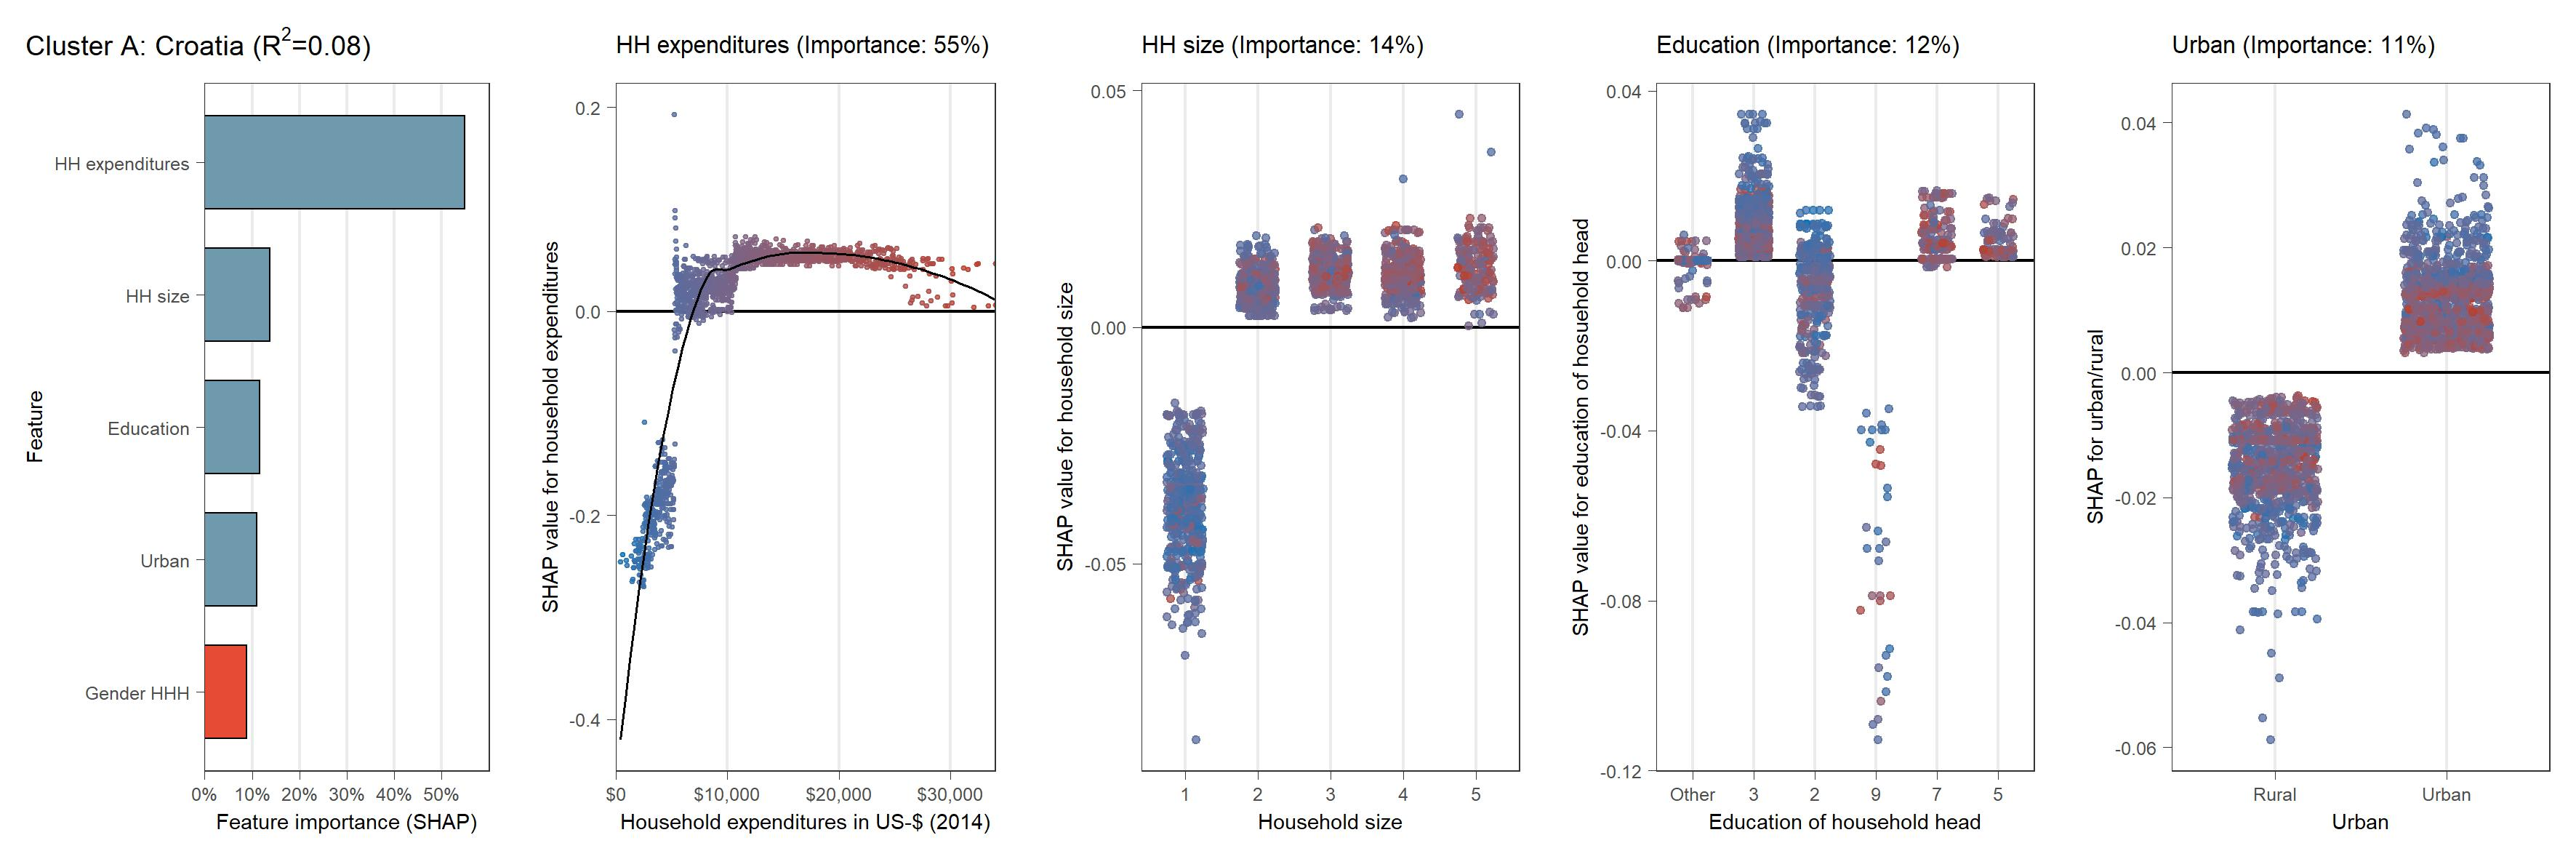
\includegraphics[width=\textwidth]{Figure_5b_HRV}
    \end{subfigure}
    \\
    \vspace{0.5cm}
    \begin{subcaption2}
     This figure shows SHAP-values for predicting carbon intensity over feature values for 87 countries in order of nine country-clusters. The bar chart displays normalized average absolute SHAP-values for all features. Features with less than 3\% of normalized SHAP-values are subsumed as "Other features (Sum)". Charts show SHAP-values over total household expenditures for all countries and for the three most important features in each country besides total household expenditures. Colors represent household expenditures with blue (red) colors indicating lower (higher) household expenditures.
     \end{subcaption2}
\end{figure}

\begin{figure}[ht!]\ContinuedFloat
    \centering
   \begin{subfigure}[b]{\textwidth}
         \centering
         \caption{Partial dependence plot (SHAP) for Romania}
         \label{fig:5b_ROU}
         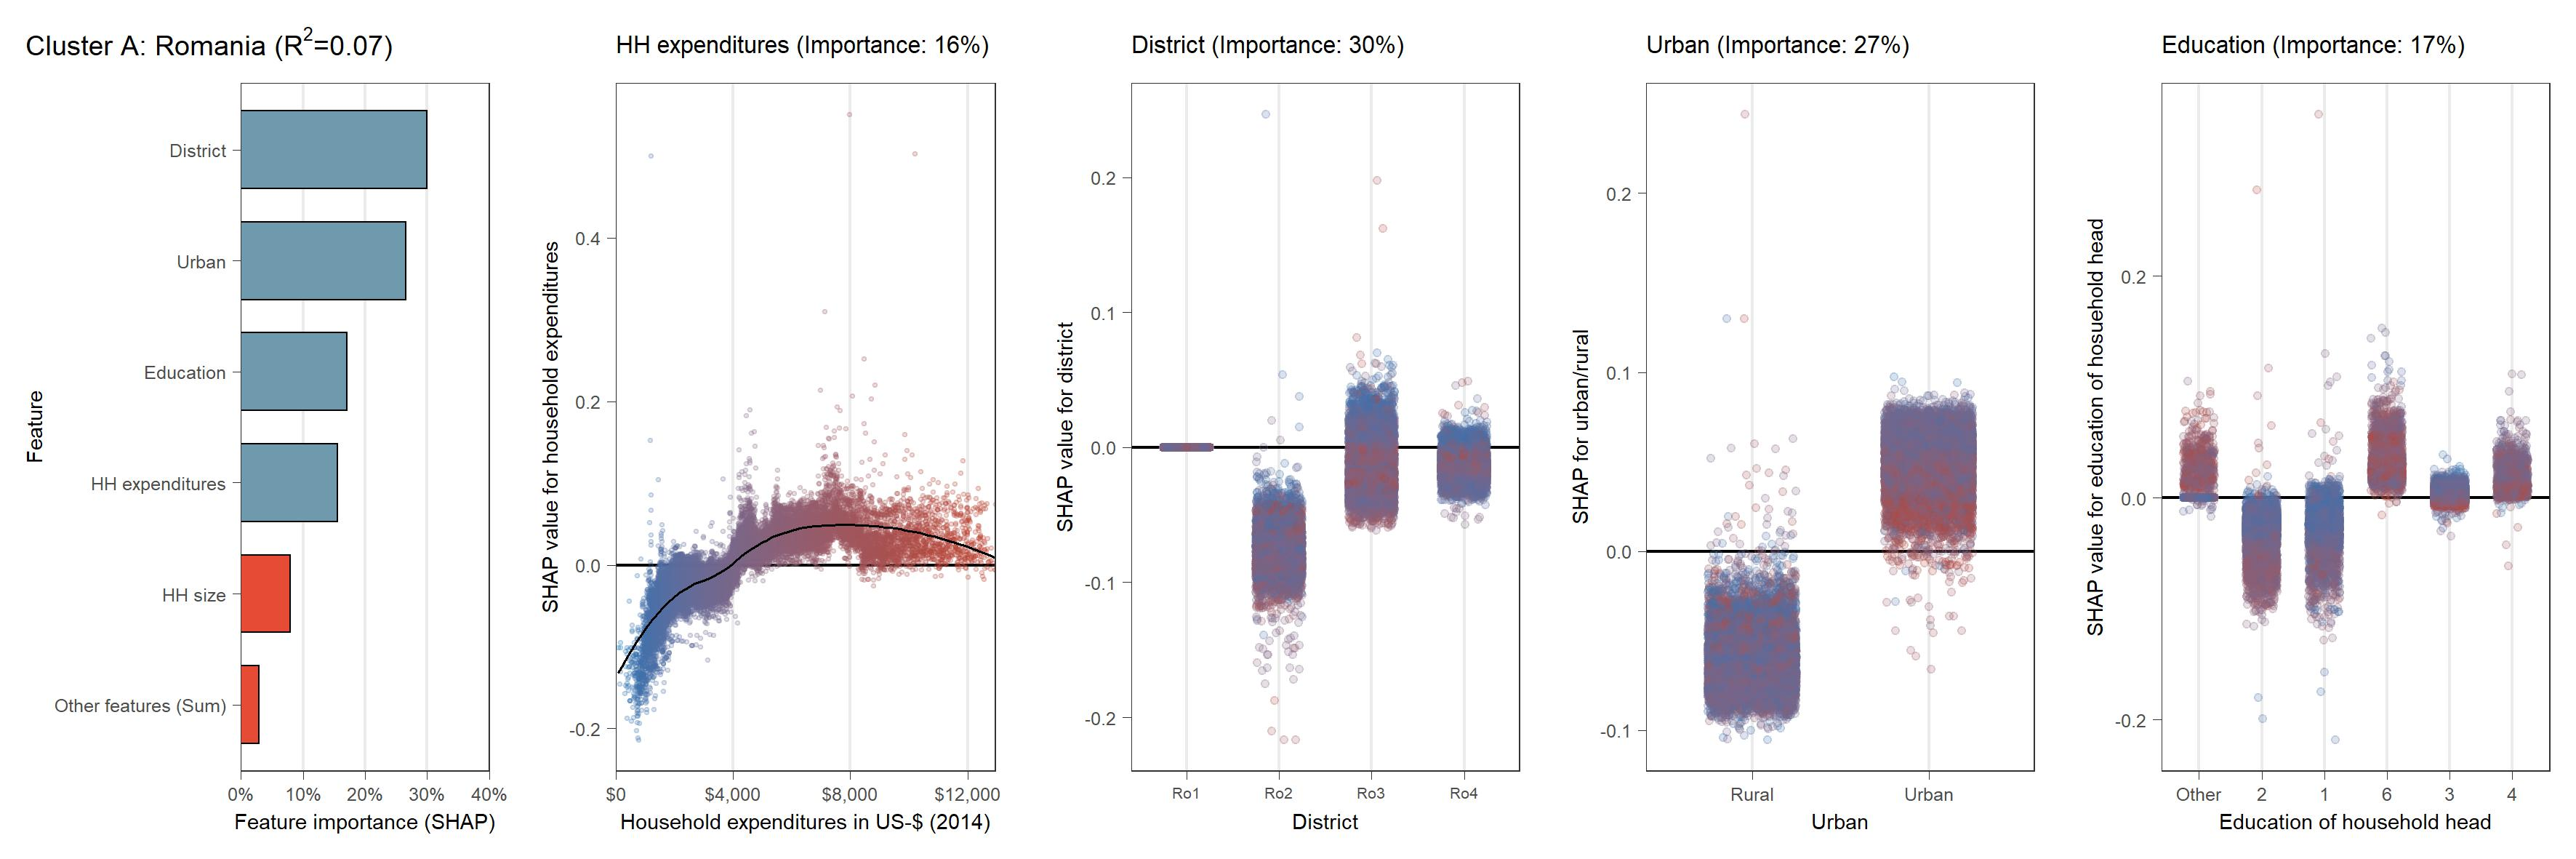
\includegraphics[width=\textwidth]{Figure_5b_ROU}         
     \end{subfigure}
    \\
    \vspace{0.5cm}
   \begin{subfigure}[b]{\textwidth}
         \centering
         \caption{Partial dependence plot (SHAP) for Switzerland}
         \label{fig:5b_CHE}
         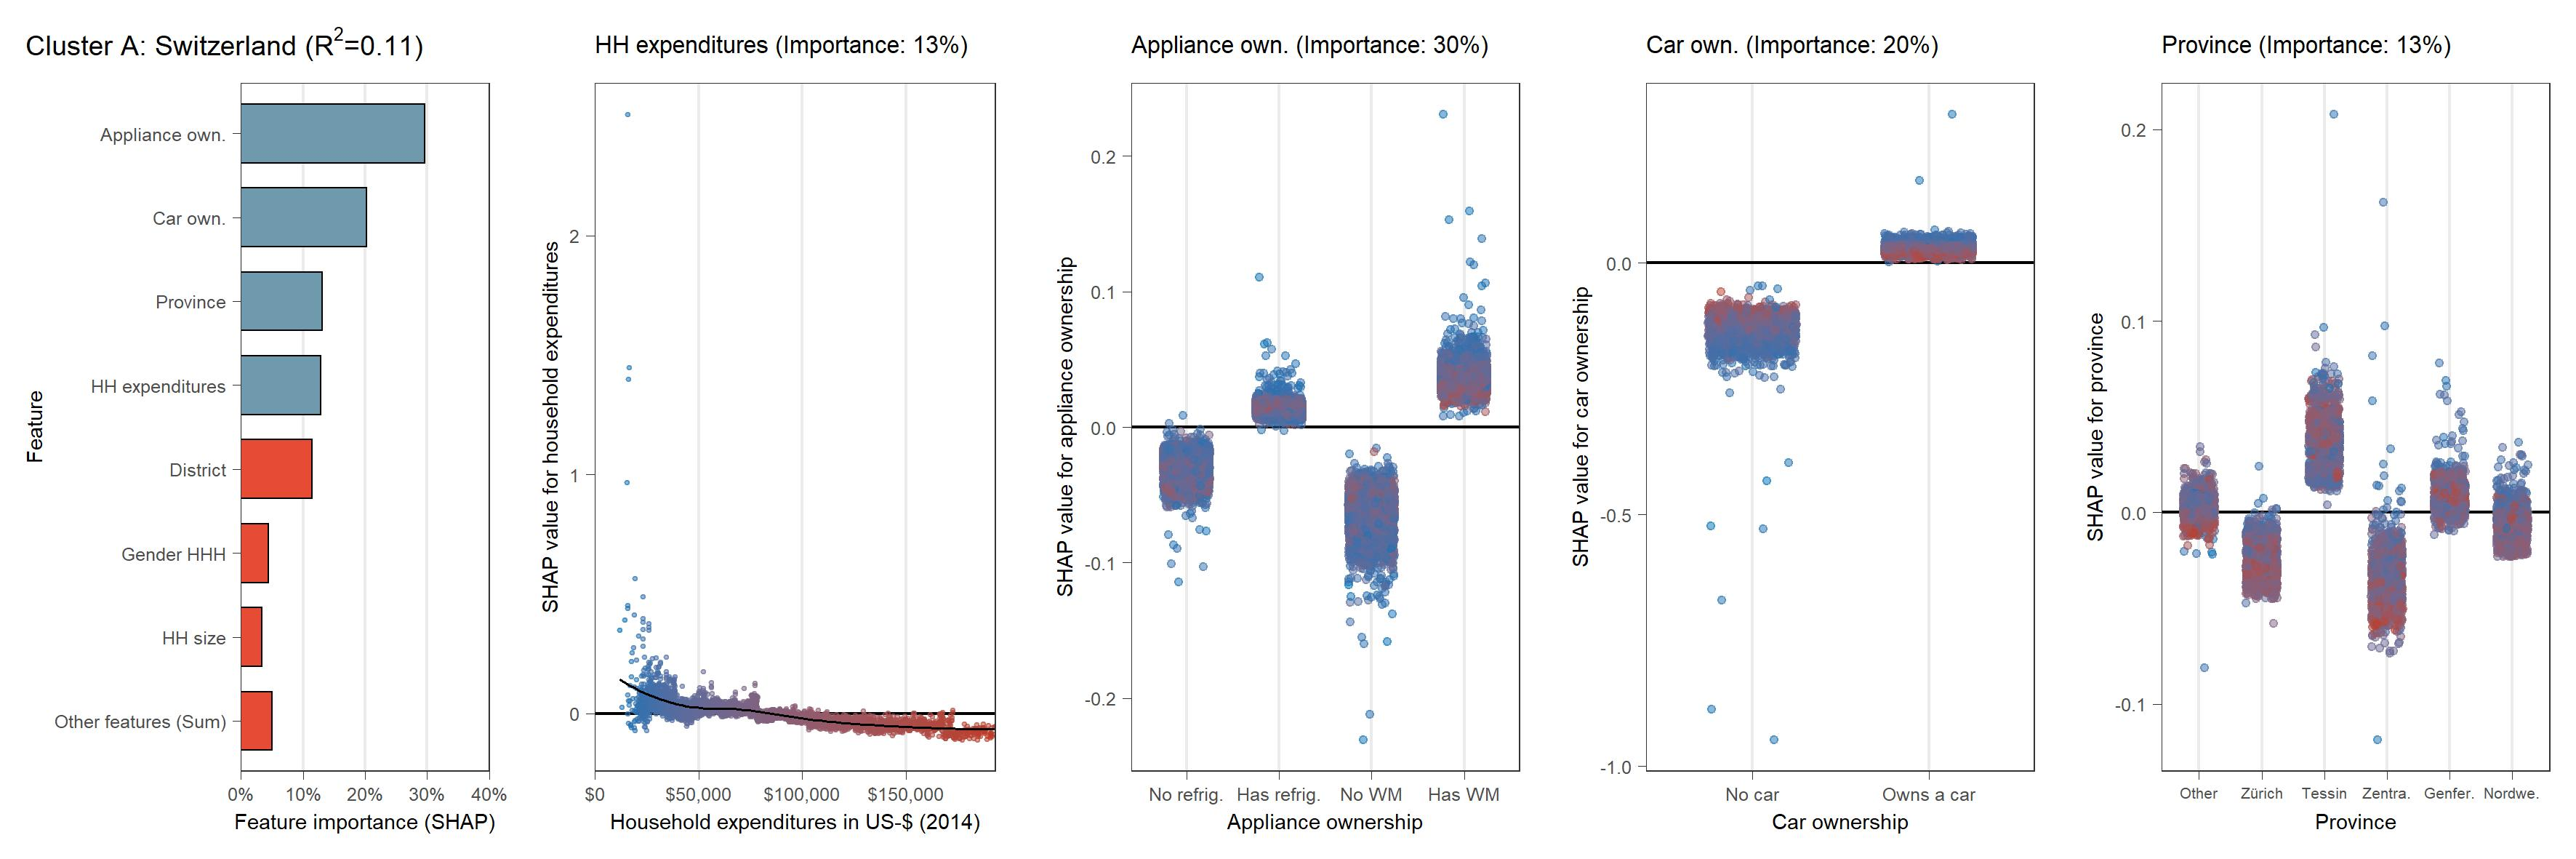
\includegraphics[width=\textwidth]{Figure_5b_CHE}         
     \end{subfigure}
    \\
    \vspace{0.5cm}
   \begin{subfigure}[b]{\textwidth}
         \centering
         \caption{Partial dependence plot (SHAP) for Poland}
         \label{fig:5b_POL}
         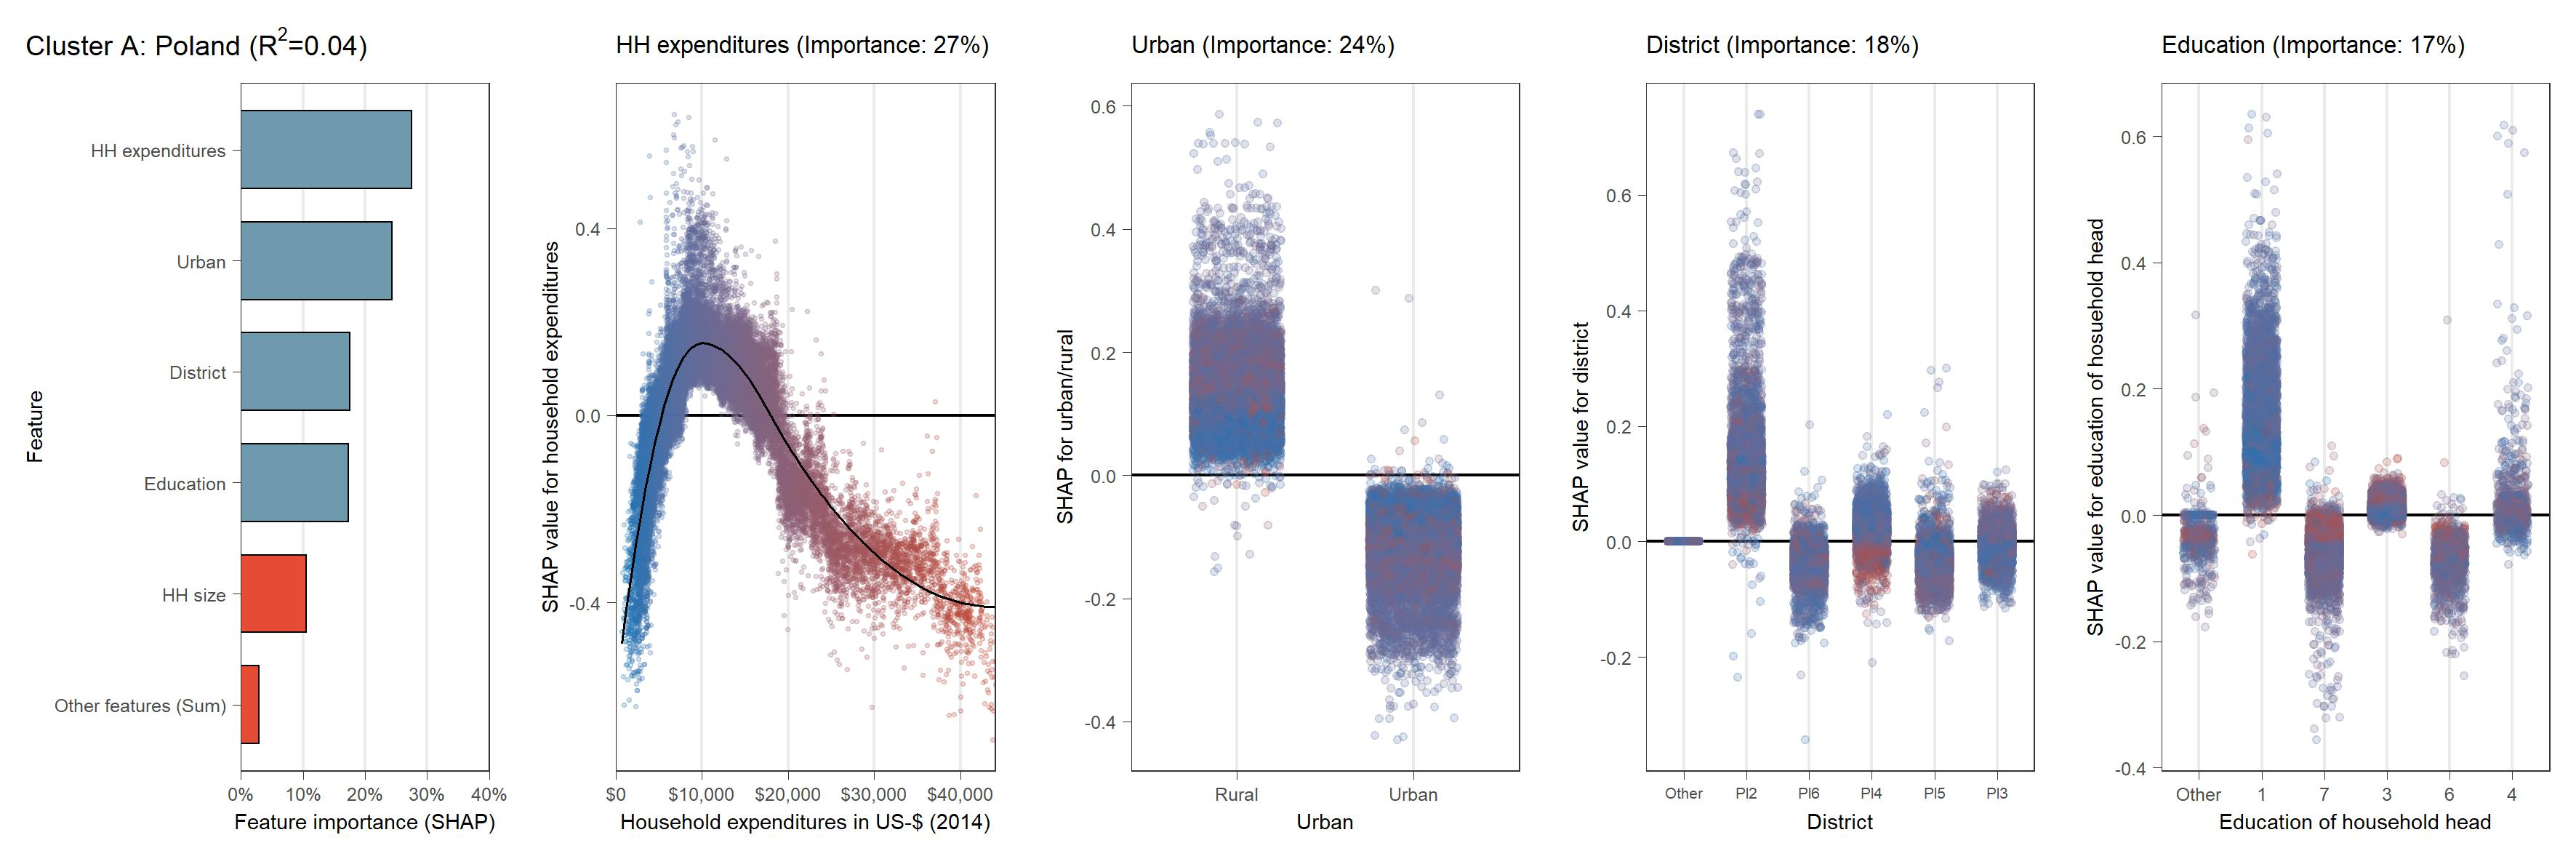
\includegraphics[width=\textwidth]{Figure_5b_POL}
    \end{subfigure}
    \\
    \vspace{0.5cm}
    \begin{subcaption2}
     This figure shows SHAP-values for predicting carbon intensity over feature values for 87 countries in order of nine country-clusters. The bar chart displays normalized average absolute SHAP-values for all features. Features with less than 3\% of normalized SHAP-values are subsumed as "Other features (Sum)". Charts show SHAP-values over total household expenditures for all countries and for the three most important features in each country besides total household expenditures. Colors represent household expenditures with blue (red) colors indicating lower (higher) household expenditures.
     \end{subcaption2}
\end{figure}

\begin{figure}[ht!]\ContinuedFloat
    \centering
   \begin{subfigure}[b]{\textwidth}
         \centering
         \caption{Partial dependence plot (SHAP) for Brazil}
         \label{fig:5b_BRA}
         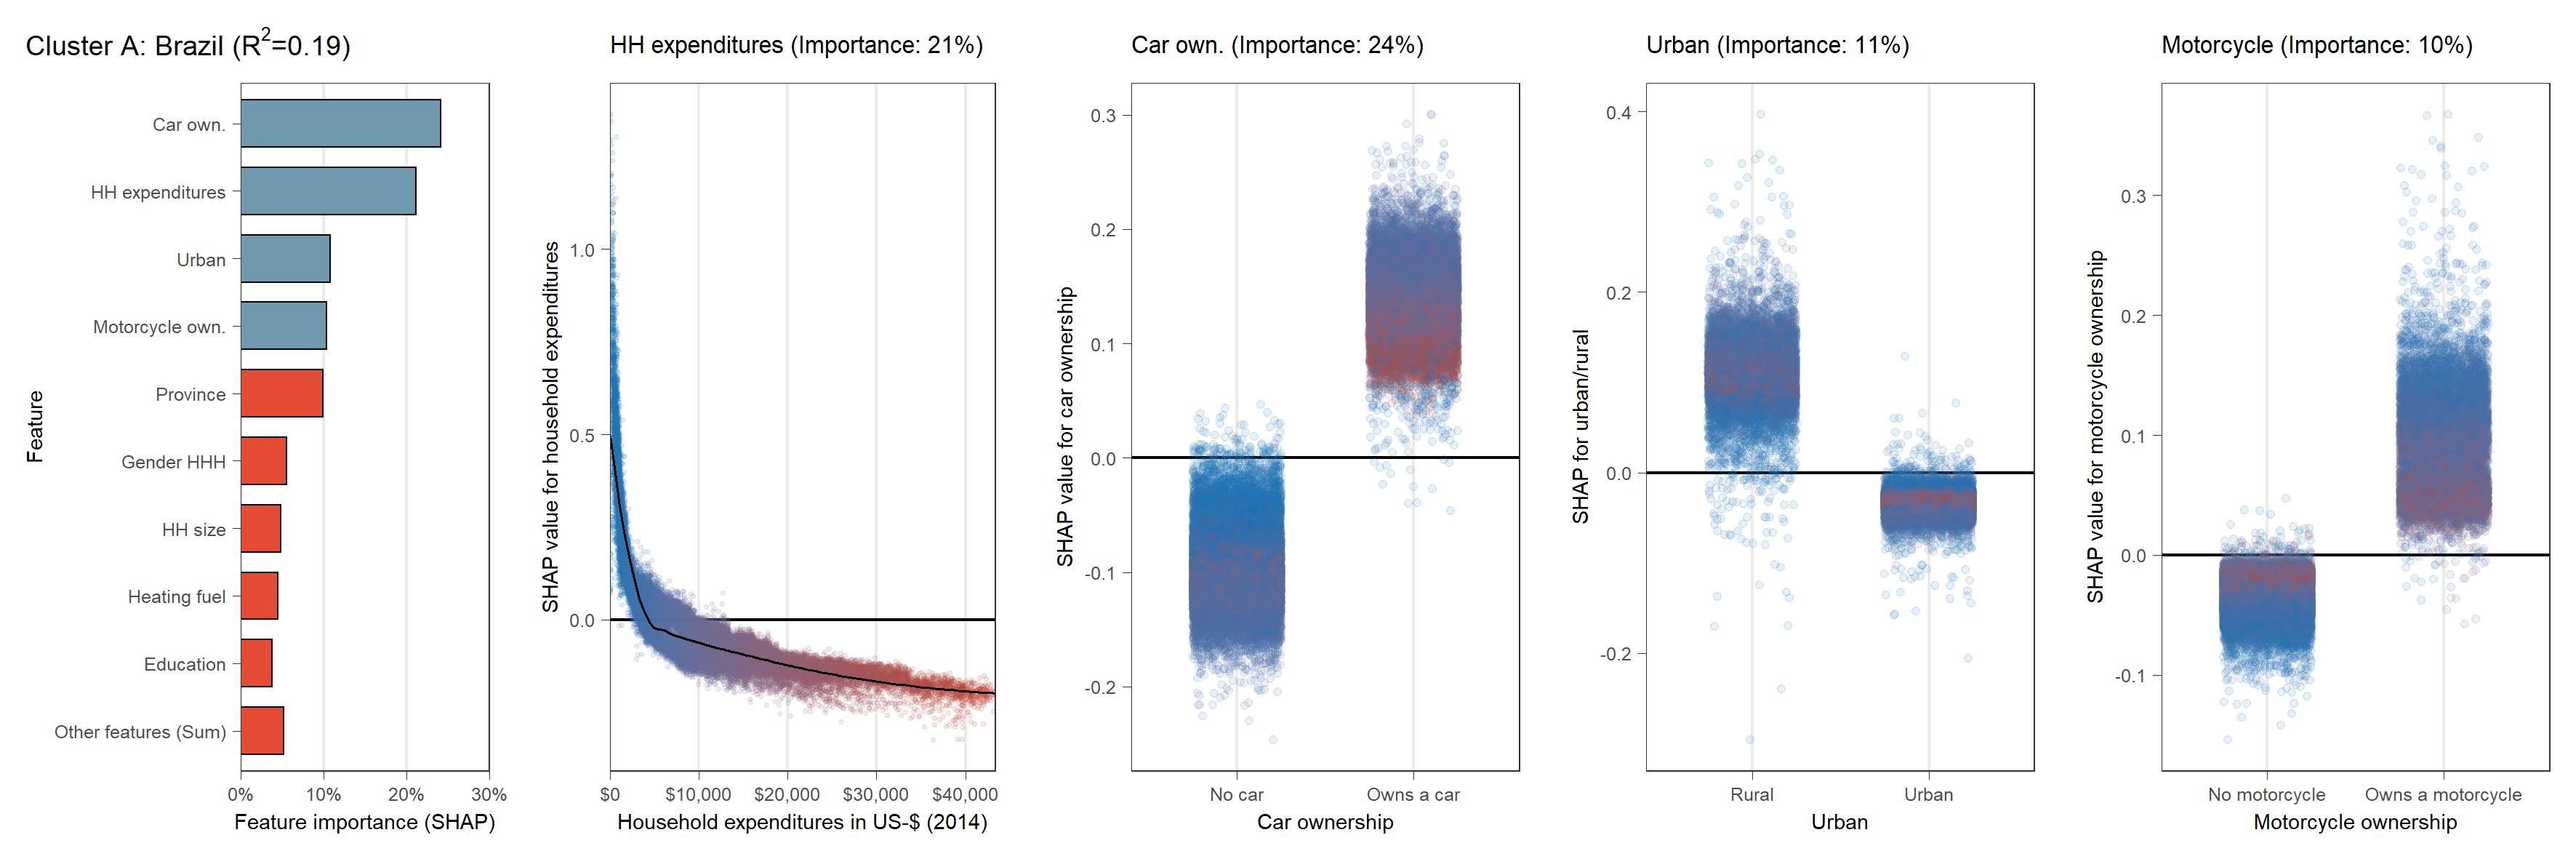
\includegraphics[width=\textwidth]{Figure_5b_BRA}         
     \end{subfigure}
    \\
    \vspace{0.5cm}
   \begin{subfigure}[b]{\textwidth}
         \centering
         \caption{Partial dependence plot (SHAP) for France}
         \label{fig:5b_FRA}
         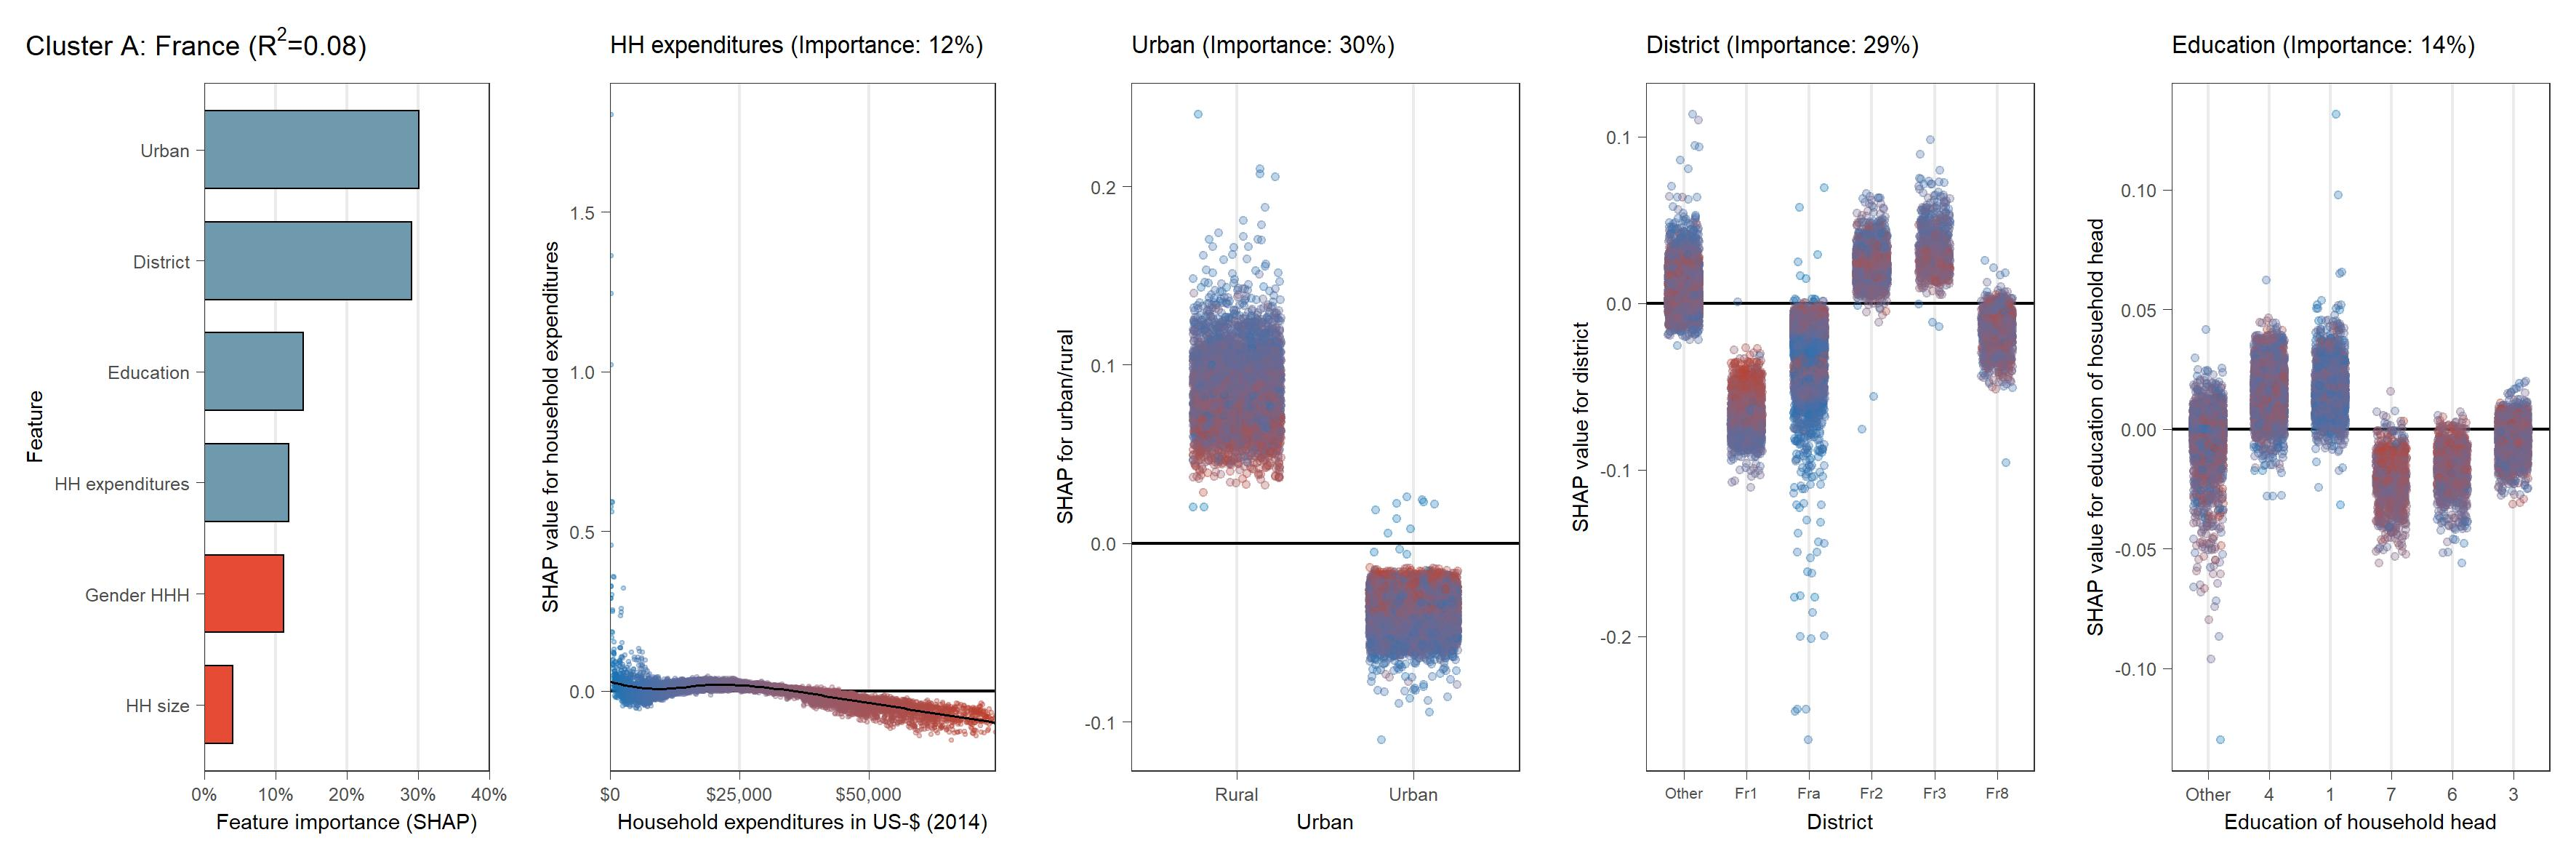
\includegraphics[width=\textwidth]{Figure_5b_FRA}         
     \end{subfigure}
    \\
    \vspace{0.5cm}
   \begin{subfigure}[b]{\textwidth}
         \centering
         \caption{Partial dependence plot (SHAP) for Austria}
         \label{fig:5b_AUT}
         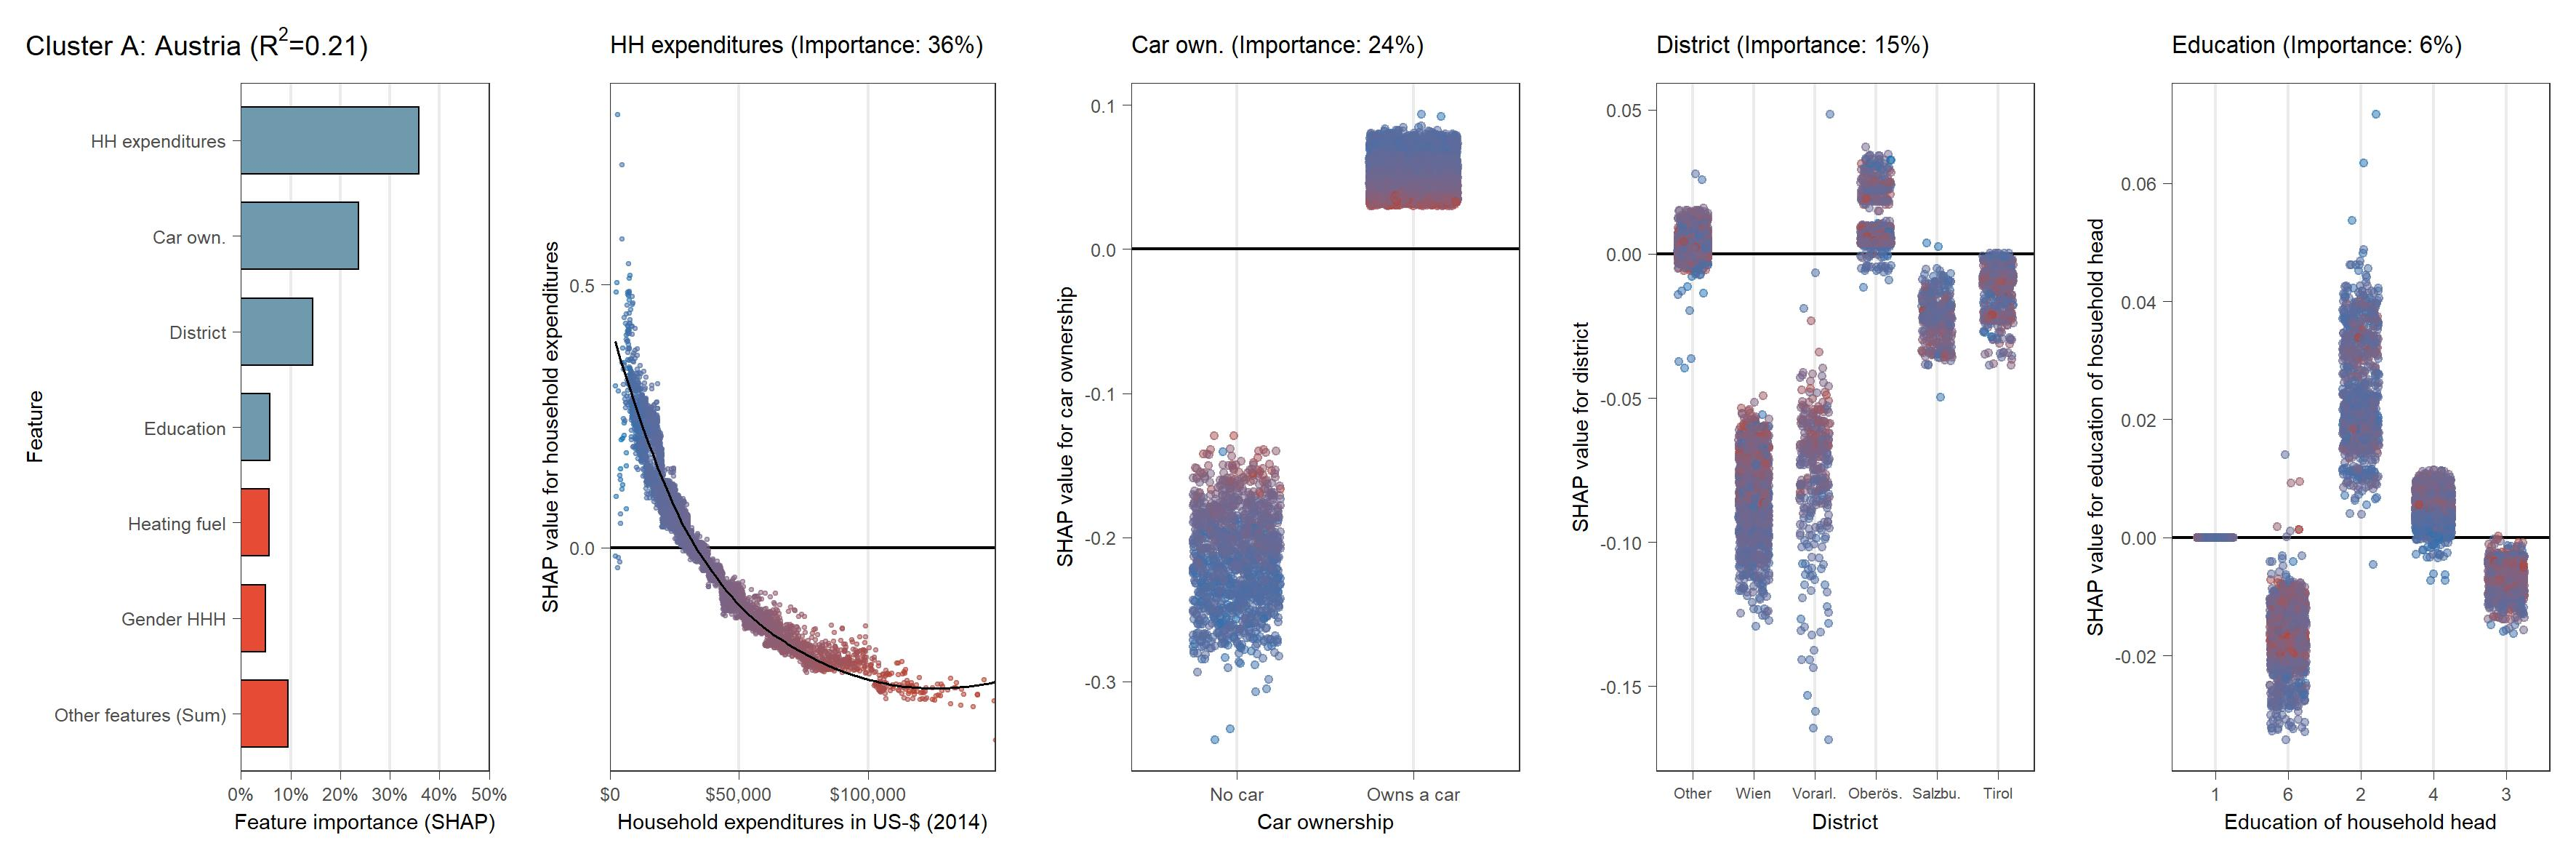
\includegraphics[width=\textwidth]{Figure_5b_AUT}
    \end{subfigure}
    \\
    \vspace{0.5cm}
    \begin{subcaption2}
     This figure shows SHAP-values for predicting carbon intensity over feature values for 87 countries in order of nine country-clusters. The bar chart displays normalized average absolute SHAP-values for all features. Features with less than 3\% of normalized SHAP-values are subsumed as "Other features (Sum)". Charts show SHAP-values over total household expenditures for all countries and for the three most important features in each country besides total household expenditures. Colors represent household expenditures with blue (red) colors indicating lower (higher) household expenditures.
     \end{subcaption2}
\end{figure}

\begin{figure}[ht!]\ContinuedFloat
    \centering
   \begin{subfigure}[b]{\textwidth}
         \centering
         \caption{Partial dependence plot (SHAP) for Denmark}
         \label{fig:5b_DNK}
         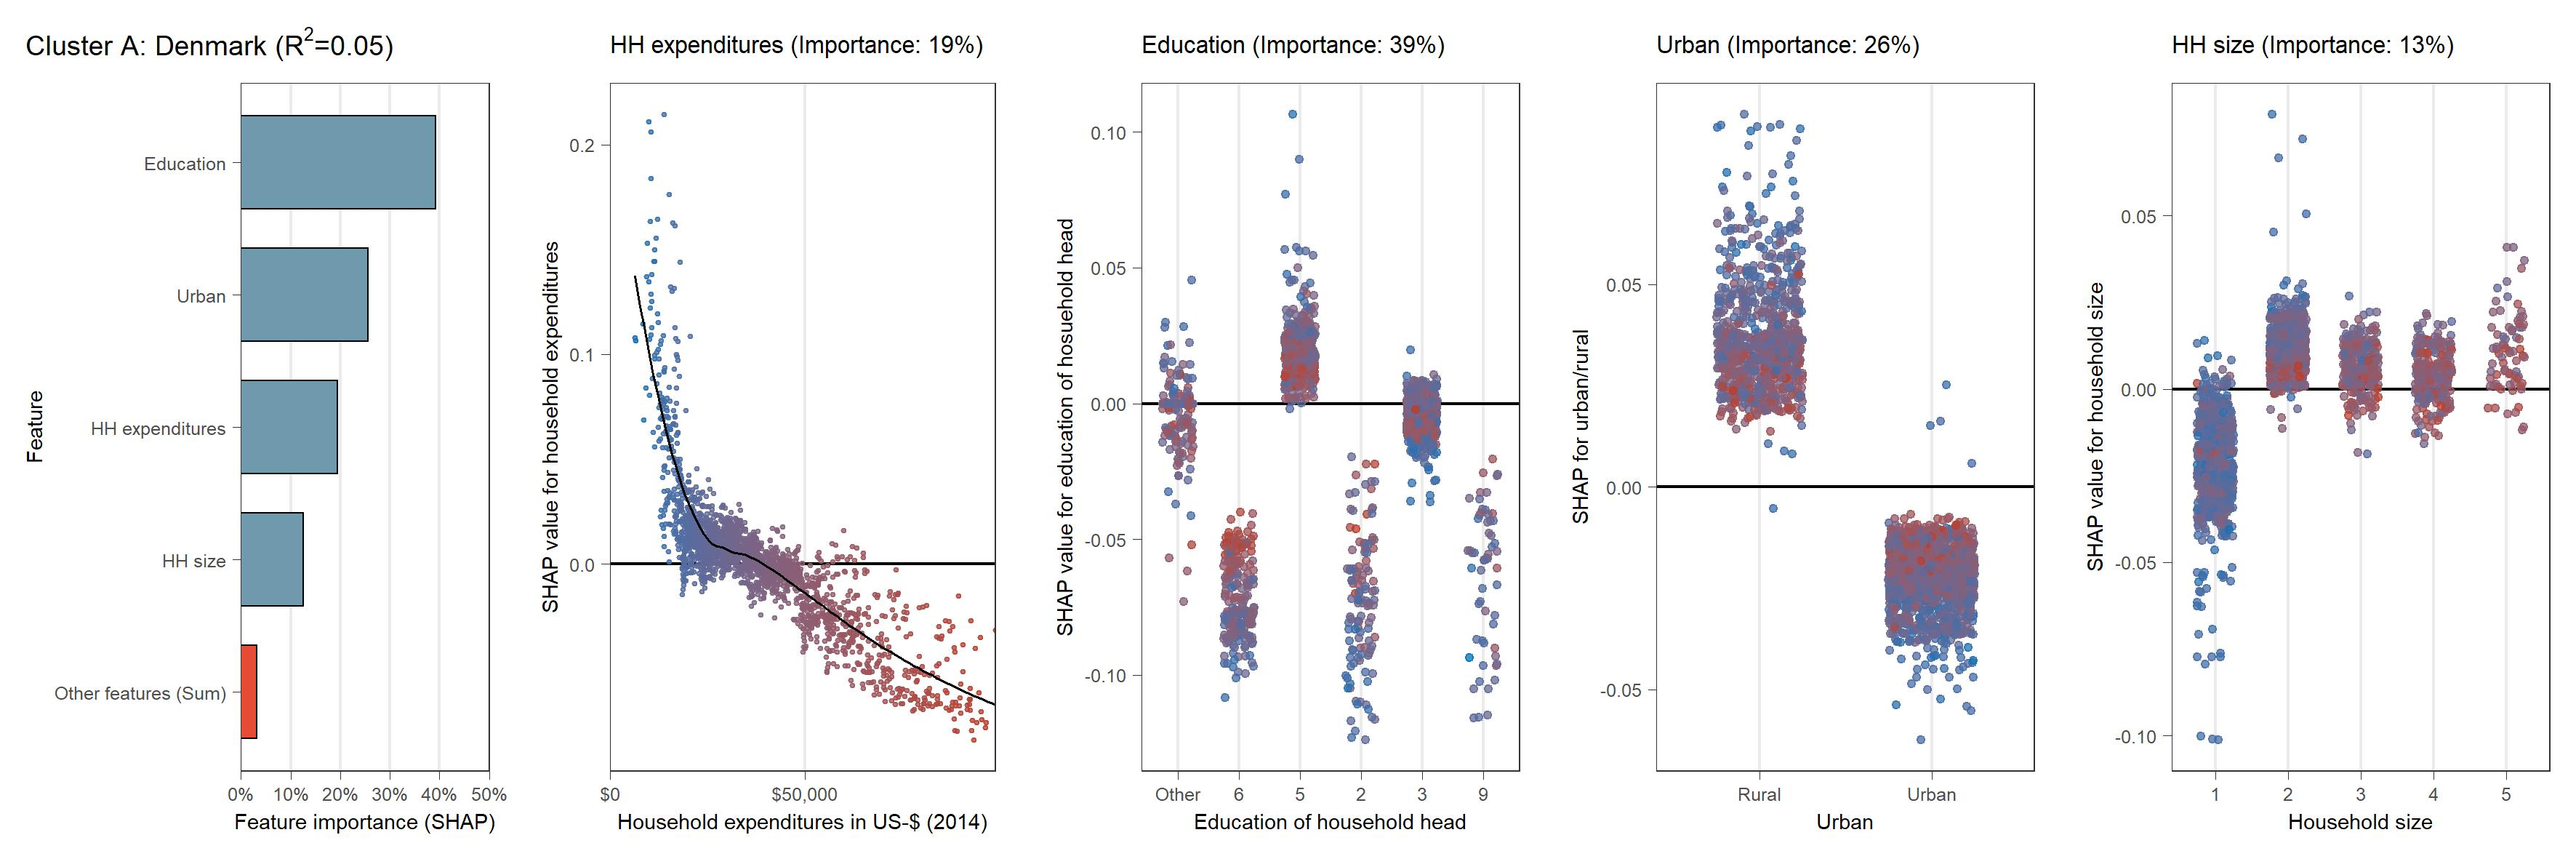
\includegraphics[width=\textwidth]{Figure_5b_DNK}         
     \end{subfigure}
    \\
    \vspace{0.5cm}
   \begin{subfigure}[b]{\textwidth}
         \centering
         \caption{Partial dependence plot (SHAP) for Lithuania}
         \label{fig:5b_LTU}
         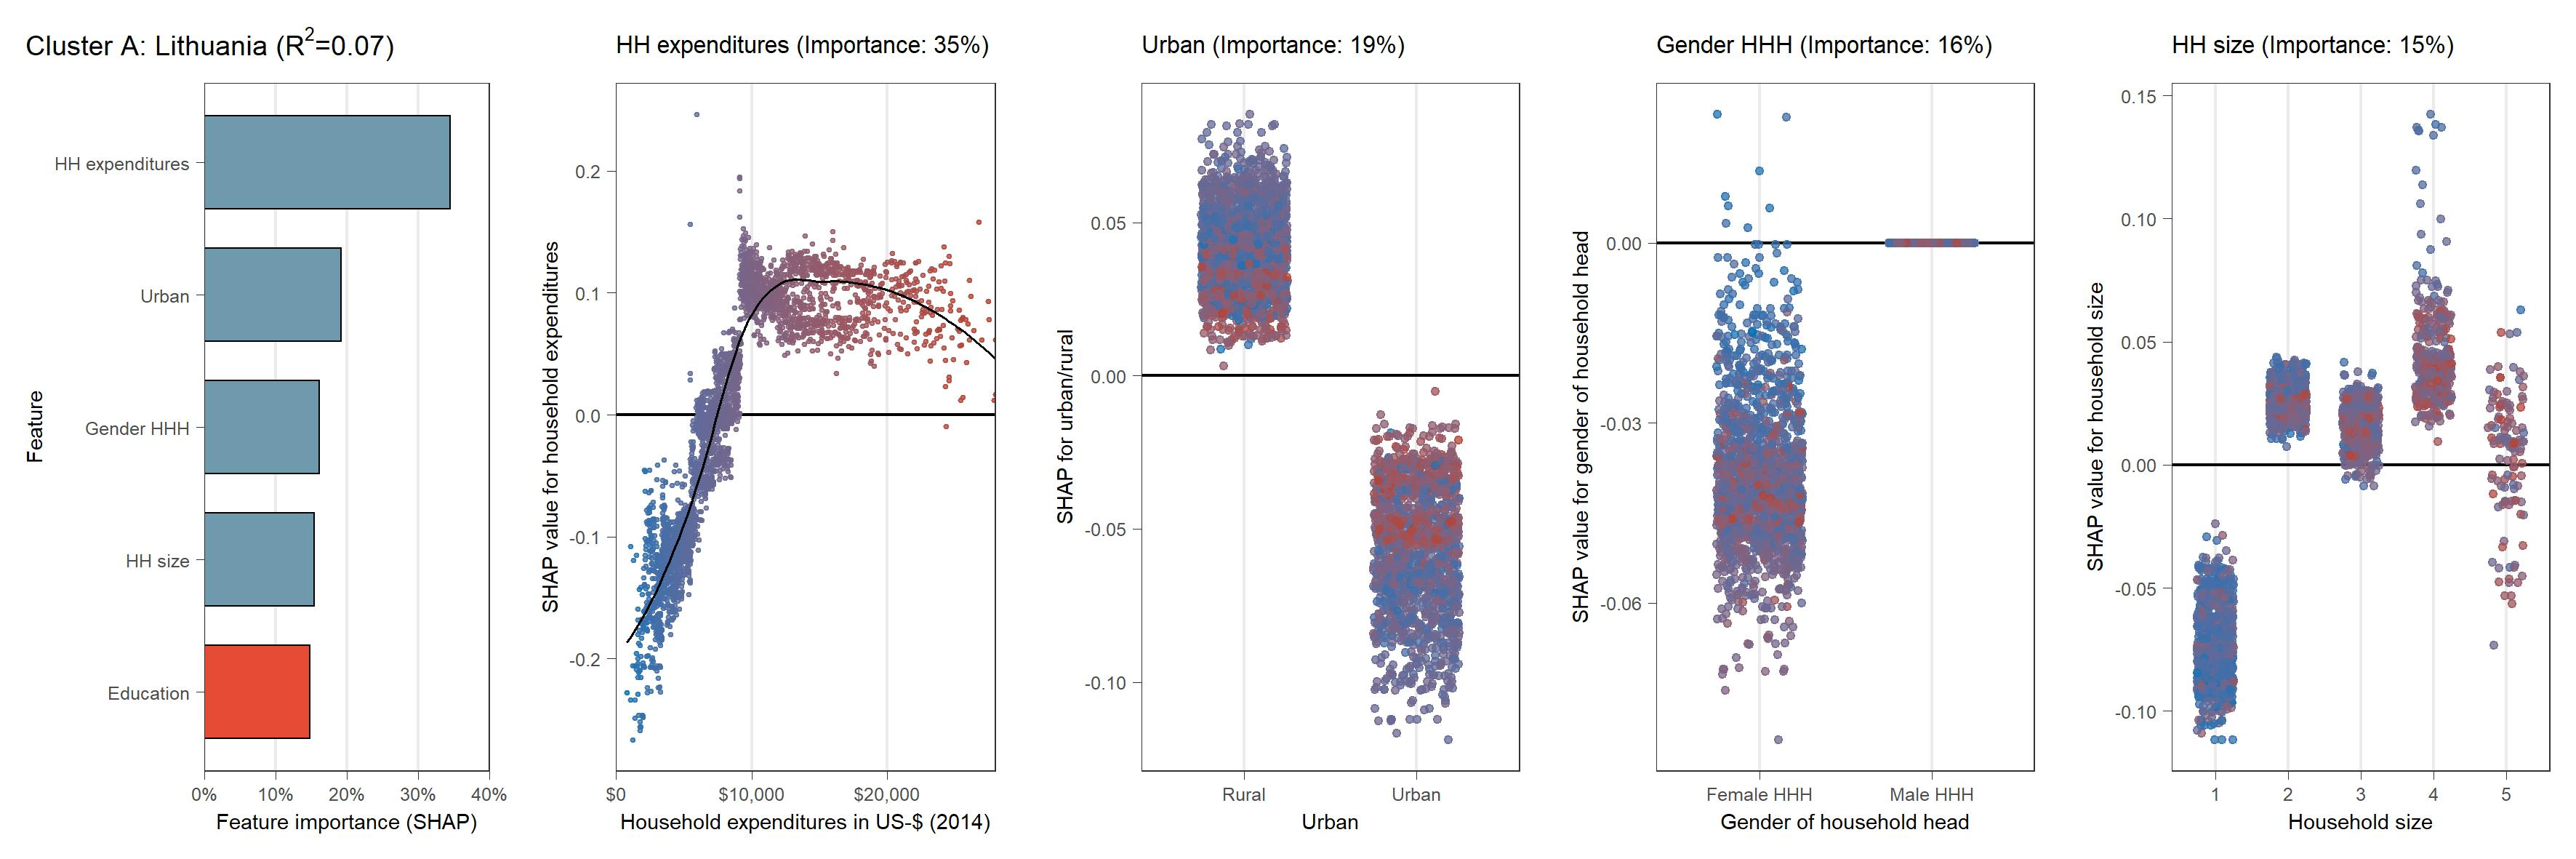
\includegraphics[width=\textwidth]{Figure_5b_LTU}         
     \end{subfigure}
    \\
    \vspace{0.5cm}
   \begin{subfigure}[b]{\textwidth}
         \centering
         \caption{Partial dependence plot (SHAP) for Cambodia}
         \label{fig:5b_KHM}
         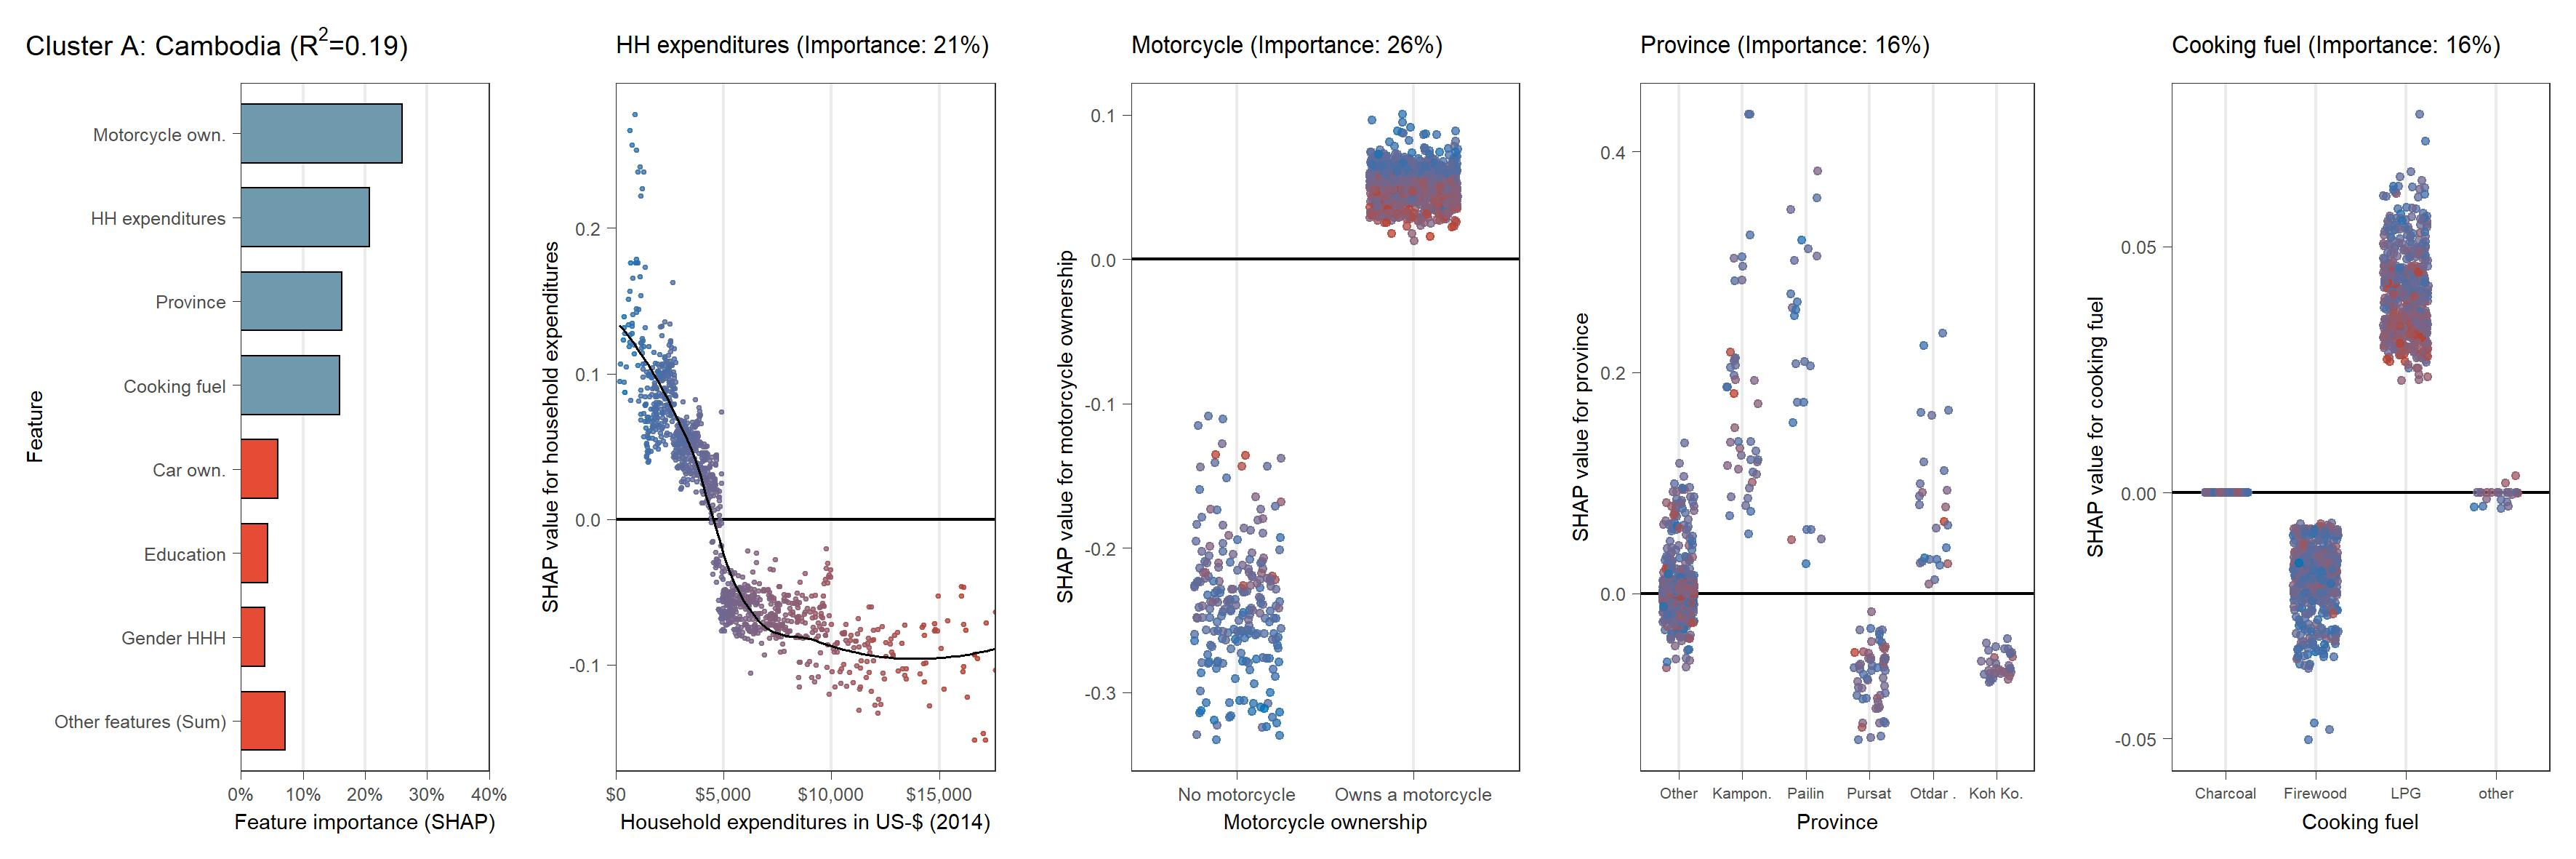
\includegraphics[width=\textwidth]{Figure_5b_KHM}
    \end{subfigure}
    \\
    \vspace{0.5cm}
    \begin{subcaption2}
     This figure shows SHAP-values for predicting carbon intensity over feature values for 87 countries in order of nine country-clusters. The bar chart displays normalized average absolute SHAP-values for all features. Features with less than 3\% of normalized SHAP-values are subsumed as "Other features (Sum)". Charts show SHAP-values over total household expenditures for all countries and for the three most important features in each country besides total household expenditures. Colors represent household expenditures with blue (red) colors indicating lower (higher) household expenditures.
     \end{subcaption2}
\end{figure}

\begin{figure}[ht!]\ContinuedFloat
    \centering
   \begin{subfigure}[b]{\textwidth}
         \centering
         \caption{Partial dependence plot (SHAP) for Finland}
         \label{fig:5b_FIN}
         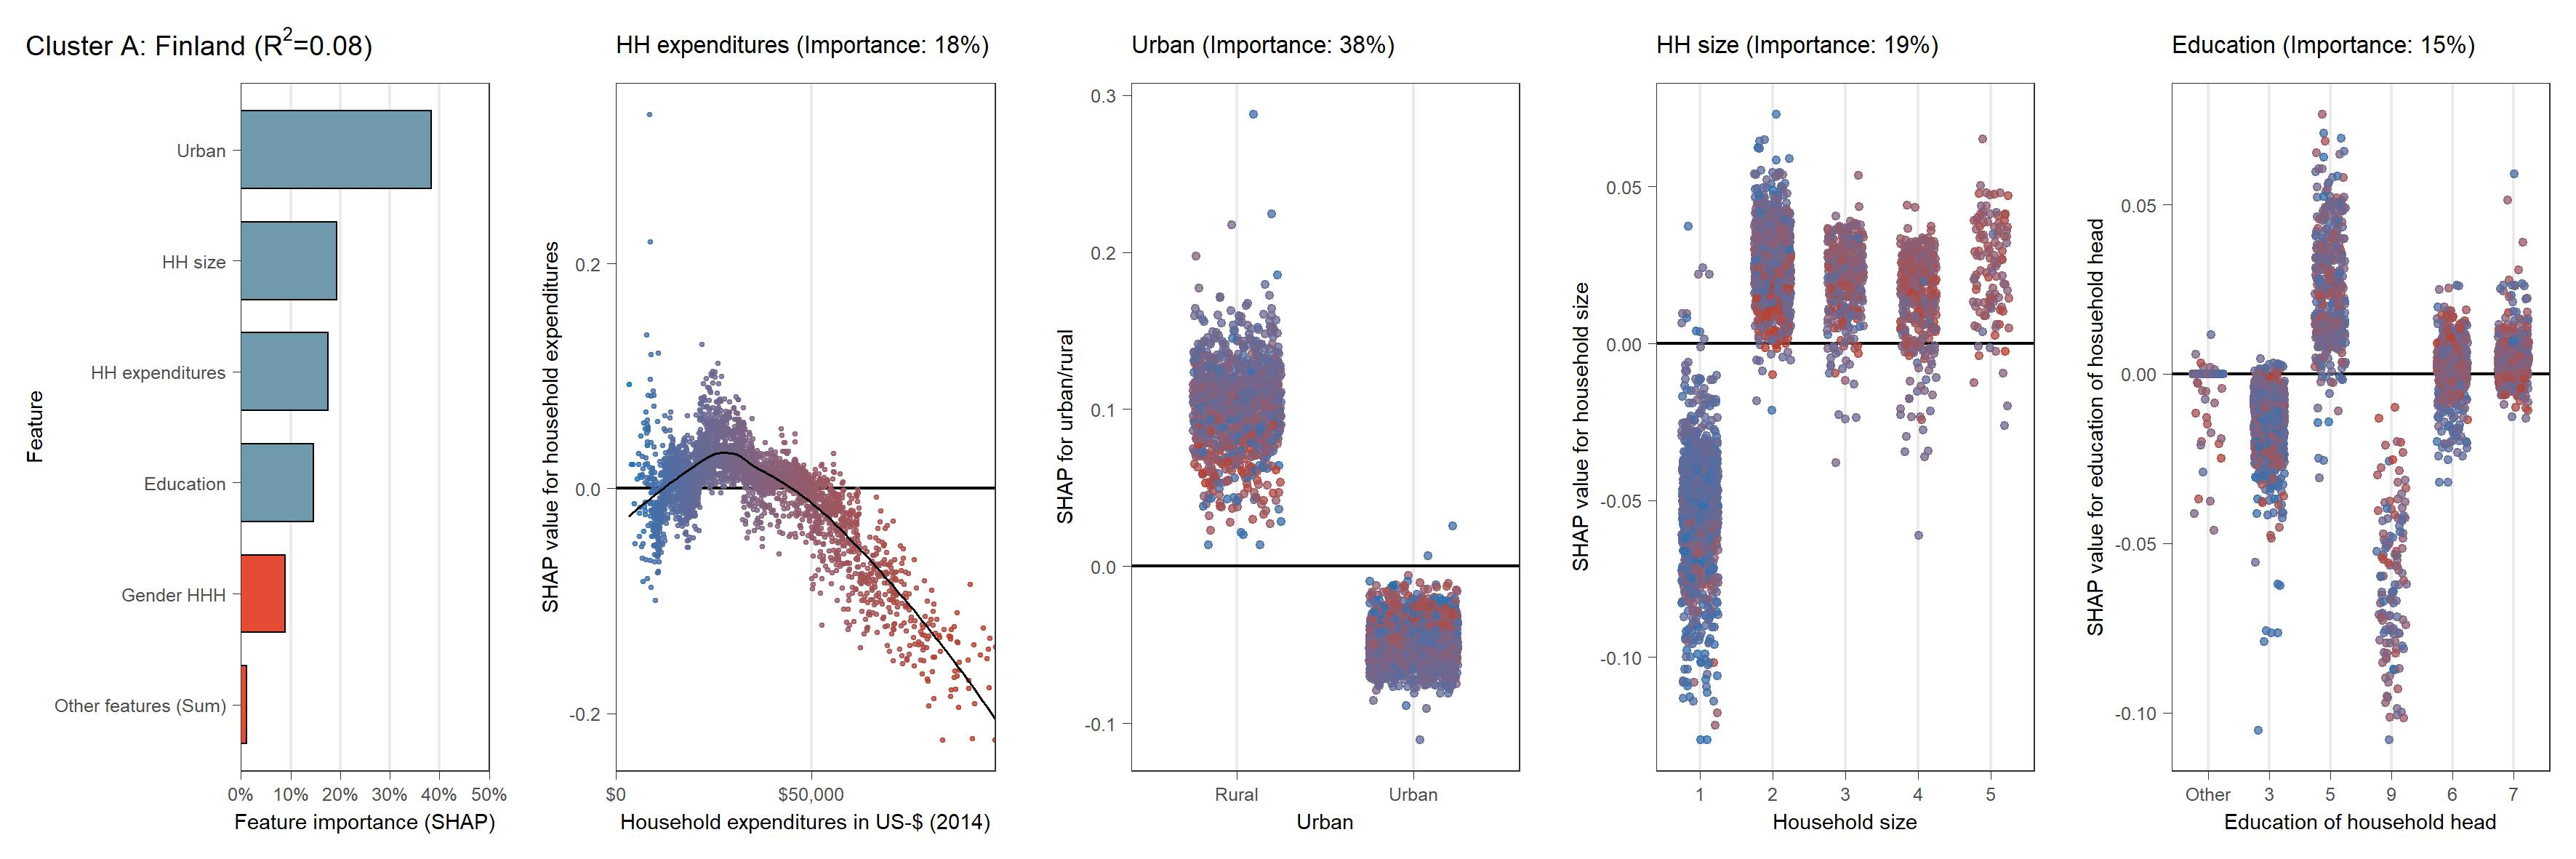
\includegraphics[width=\textwidth]{Figure_5b_FIN}         
     \end{subfigure}
    \\
    \vspace{0.5cm}
   \begin{subfigure}[b]{\textwidth}
         \centering
         \caption{Partial dependence plot (SHAP) for Colombia}
         \label{fig:5b_COL}
         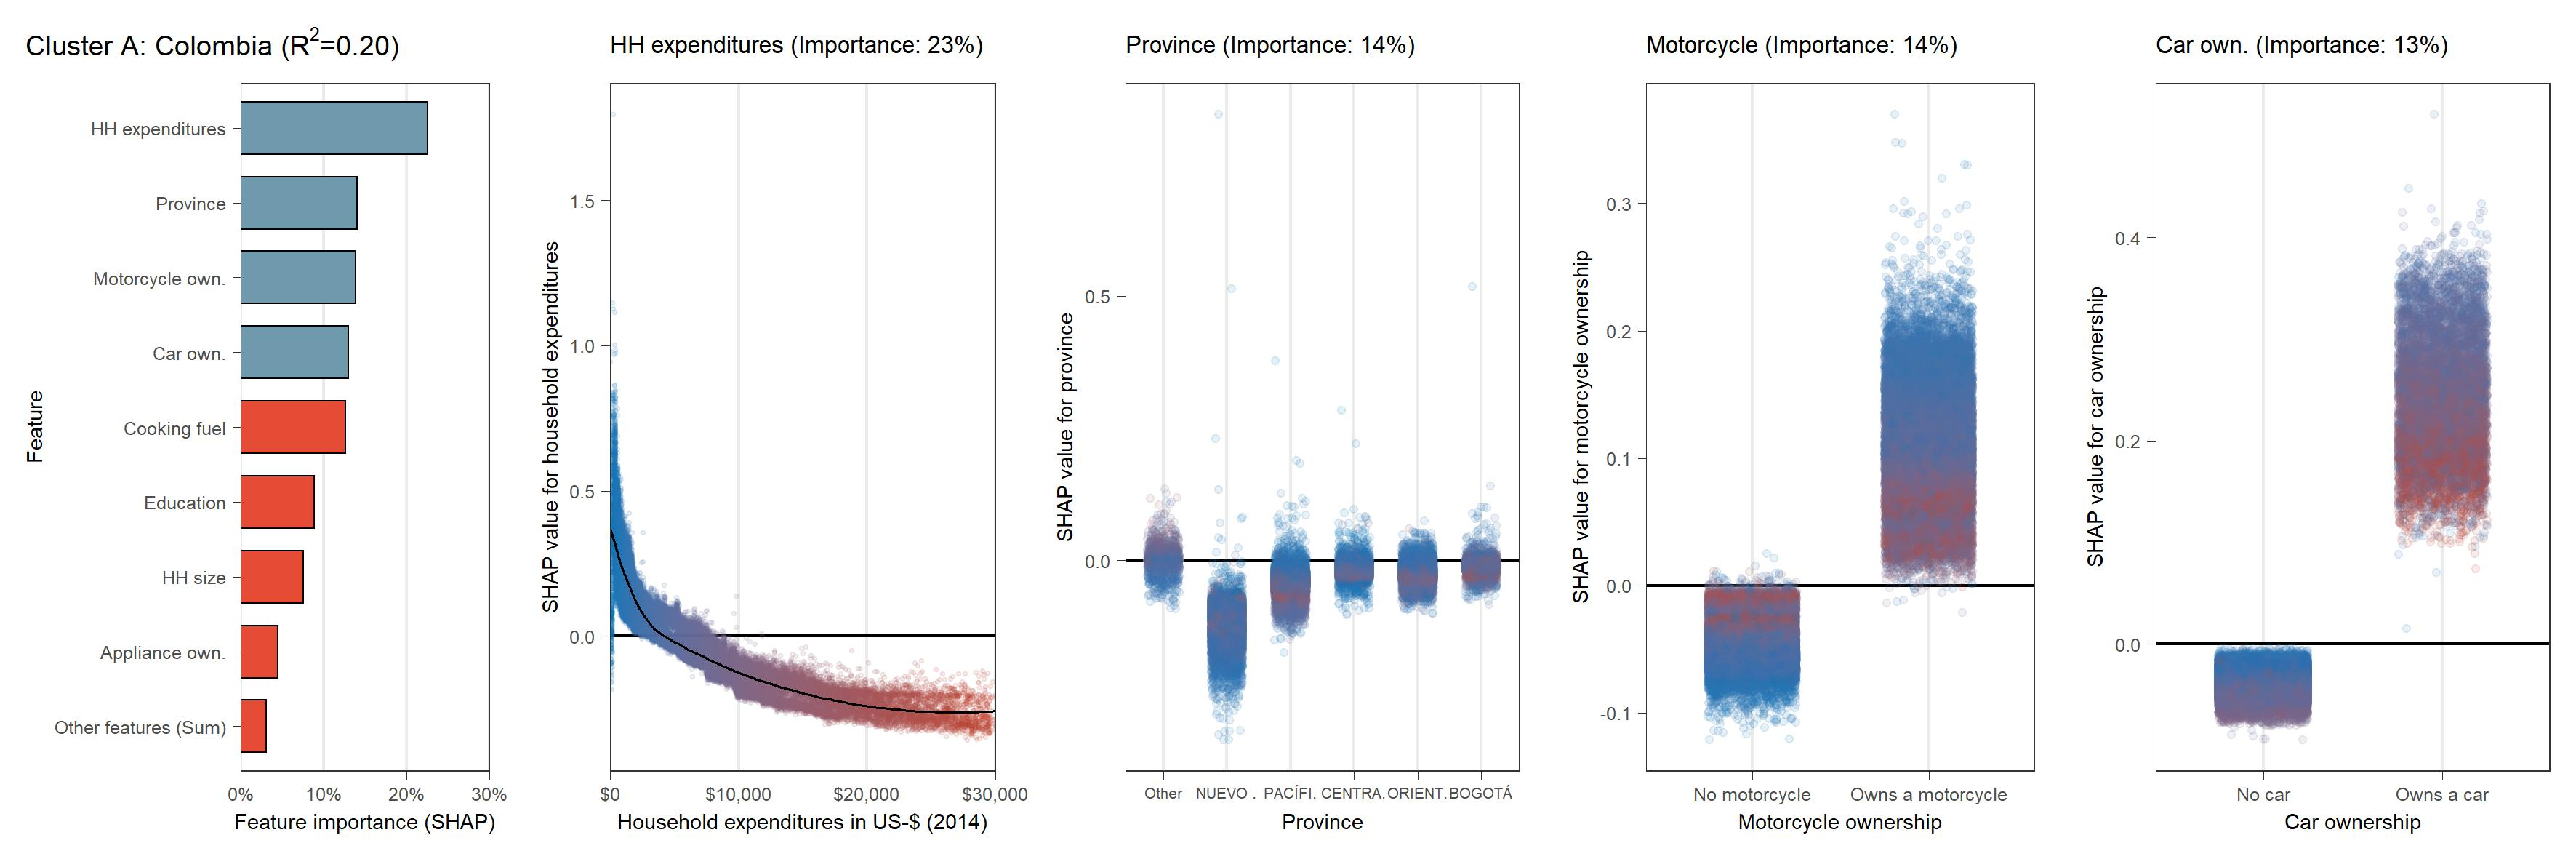
\includegraphics[width=\textwidth]{Figure_5b_COL}         
     \end{subfigure}
    \\
    \vspace{0.5cm}
   \begin{subfigure}[b]{\textwidth}
         \centering
         \caption{Partial dependence plot (SHAP) for Spain}
         \label{fig:5b_ESP}
         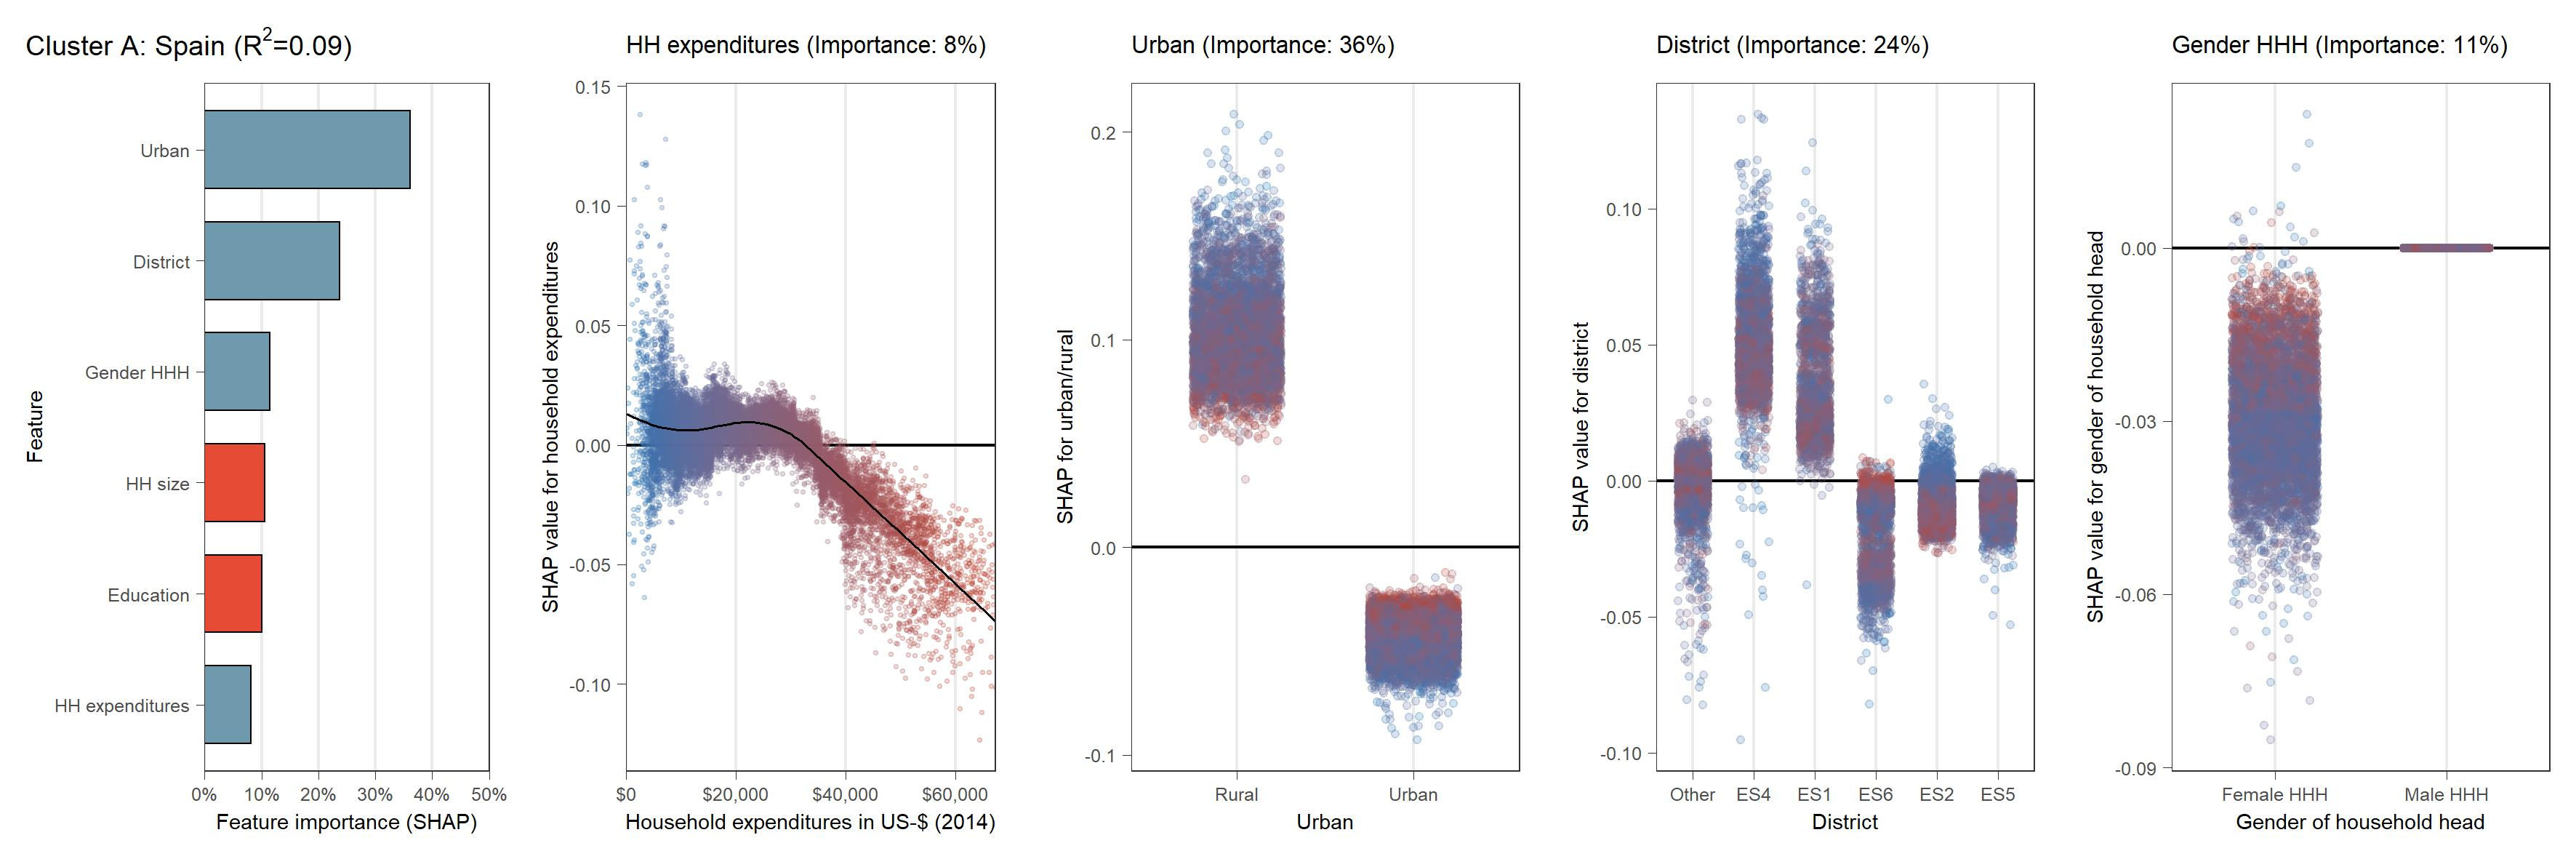
\includegraphics[width=\textwidth]{Figure_5b_ESP}
    \end{subfigure}
    \\
    \vspace{0.5cm}
    \begin{subcaption2}
     This figure shows SHAP-values for predicting carbon intensity over feature values for 87 countries in order of nine country-clusters. The bar chart displays normalized average absolute SHAP-values for all features. Features with less than 3\% of normalized SHAP-values are subsumed as "Other features (Sum)". Charts show SHAP-values over total household expenditures for all countries and for the three most important features in each country besides total household expenditures. Colors represent household expenditures with blue (red) colors indicating lower (higher) household expenditures.
     \end{subcaption2}
\end{figure}

\begin{figure}[ht!]\ContinuedFloat
    \centering
   \begin{subfigure}[b]{\textwidth}
         \centering
         \caption{Partial dependence plot (SHAP) for USA}
         \label{fig:5b_USA}
         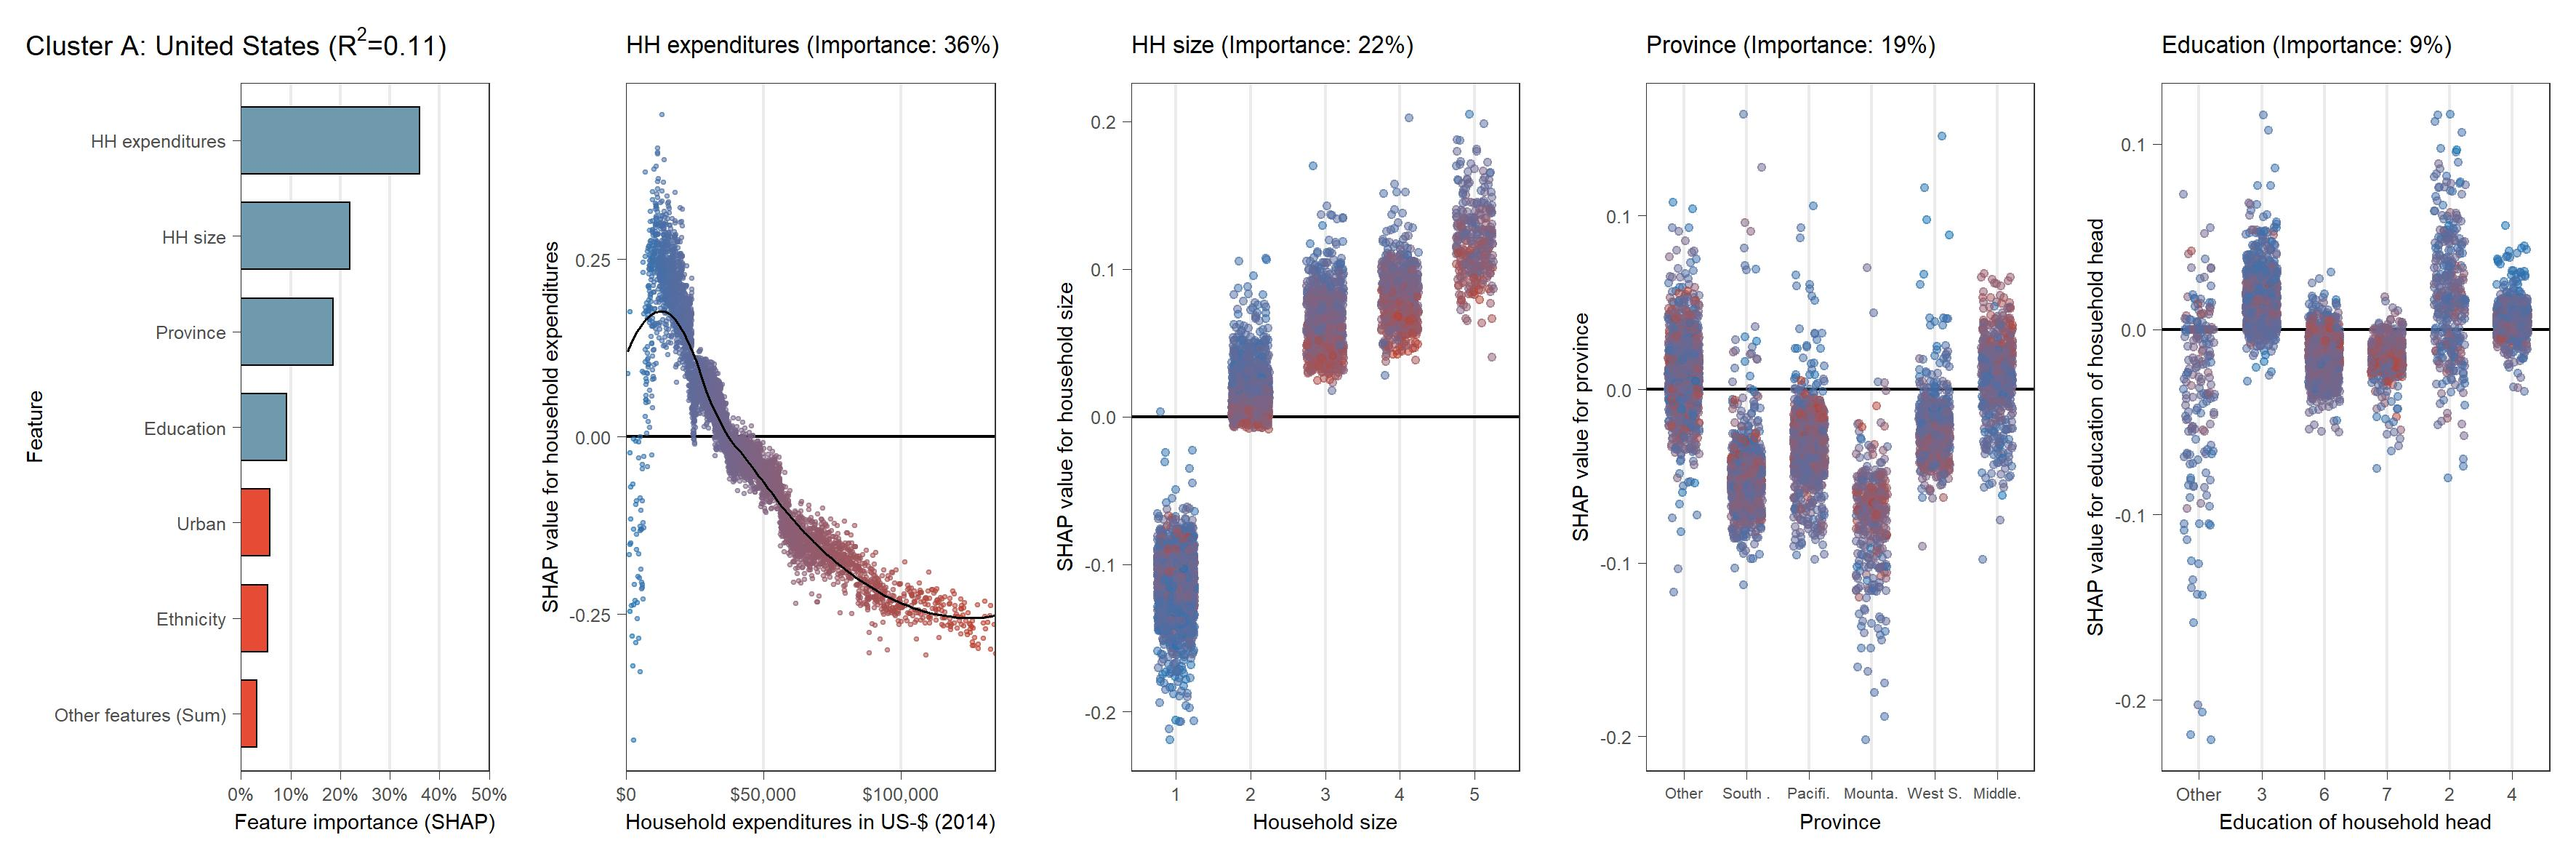
\includegraphics[width=\textwidth]{Figure_5b_USA}         
     \end{subfigure}
    \\
    \vspace{0.5cm}
   \begin{subfigure}[b]{\textwidth}
         \centering
         \caption{Partial dependence plot (SHAP) for Belgium}
         \label{fig:5b_BEL}
         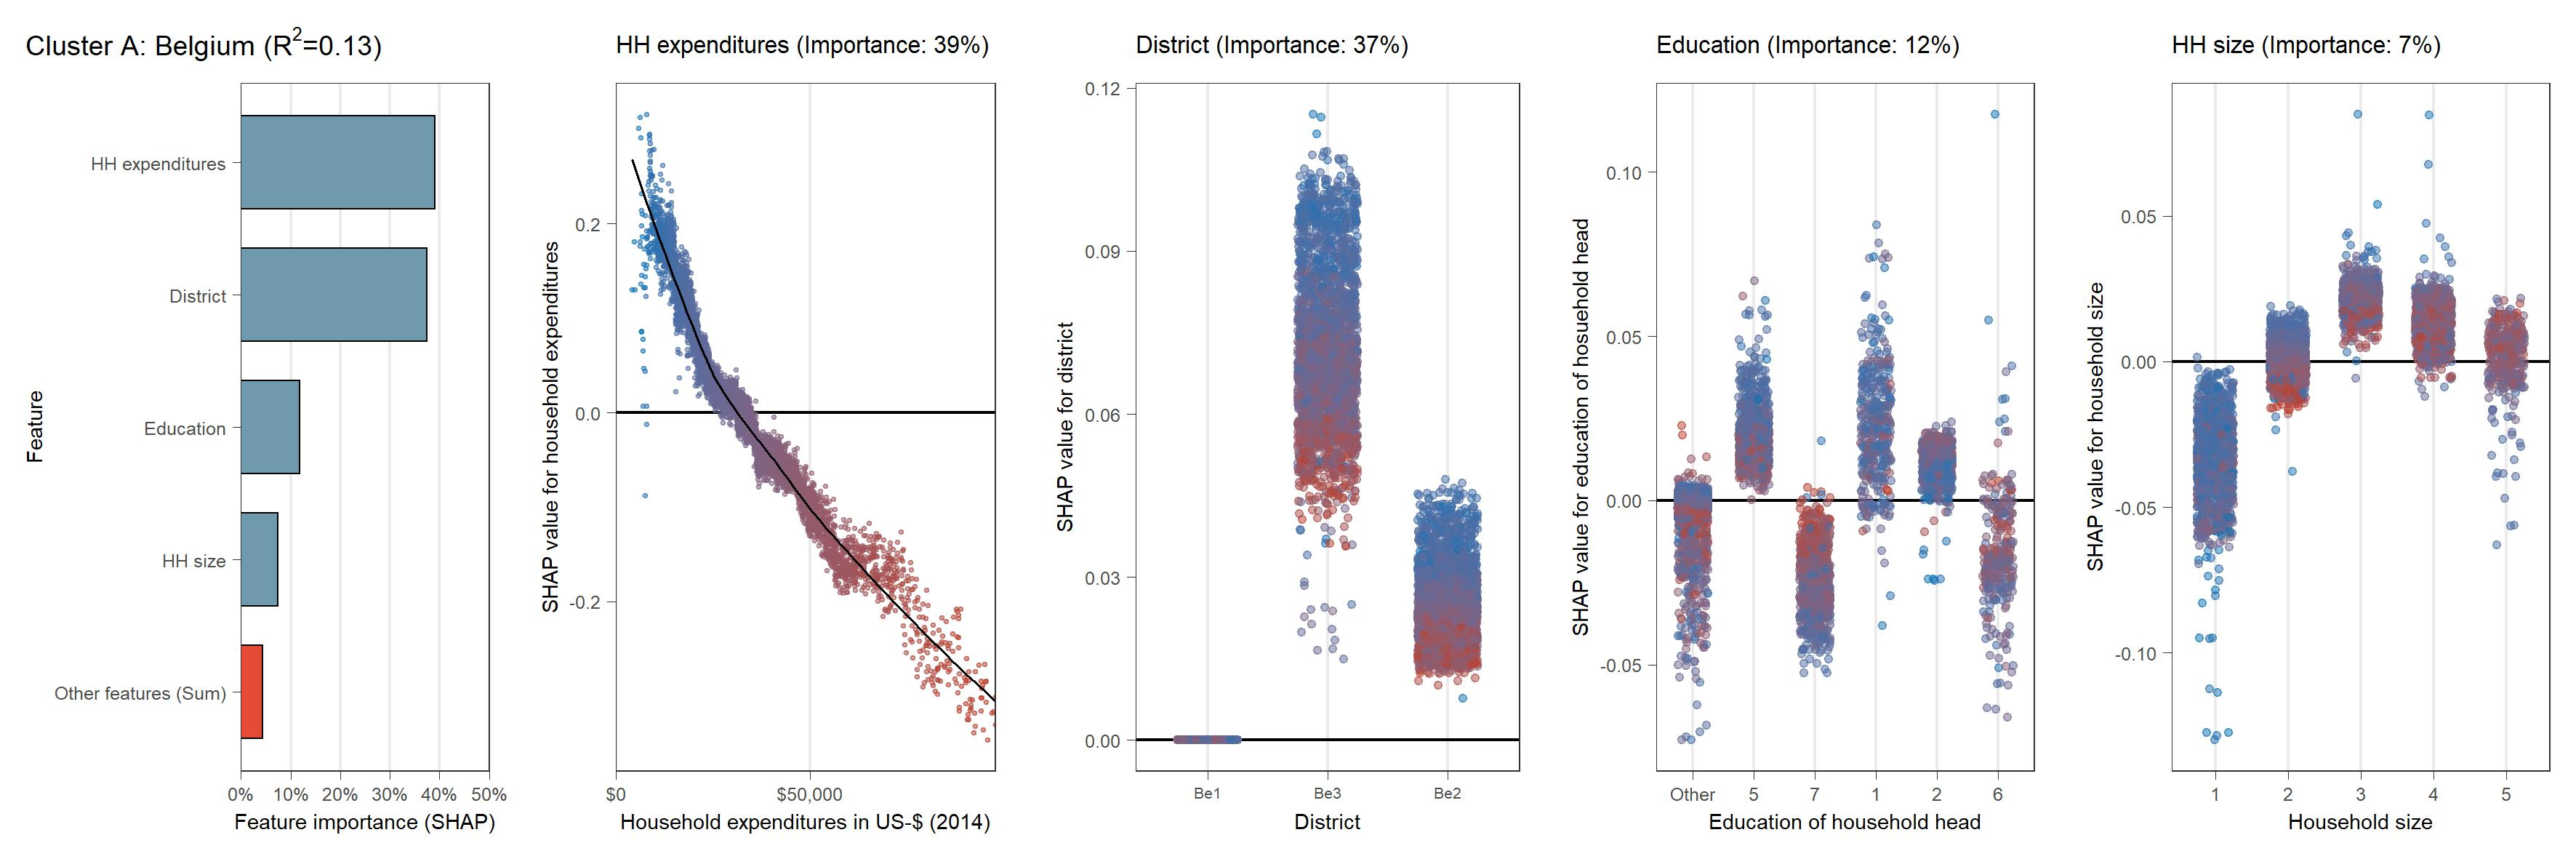
\includegraphics[width=\textwidth]{Figure_5b_BEL}         
     \end{subfigure}
    \\
    \vspace{0.5cm}
   \begin{subfigure}[b]{\textwidth}
         \centering
         \caption{Partial dependence plot (SHAP) for United Kingdom}
         \label{fig:5b_GBR}
         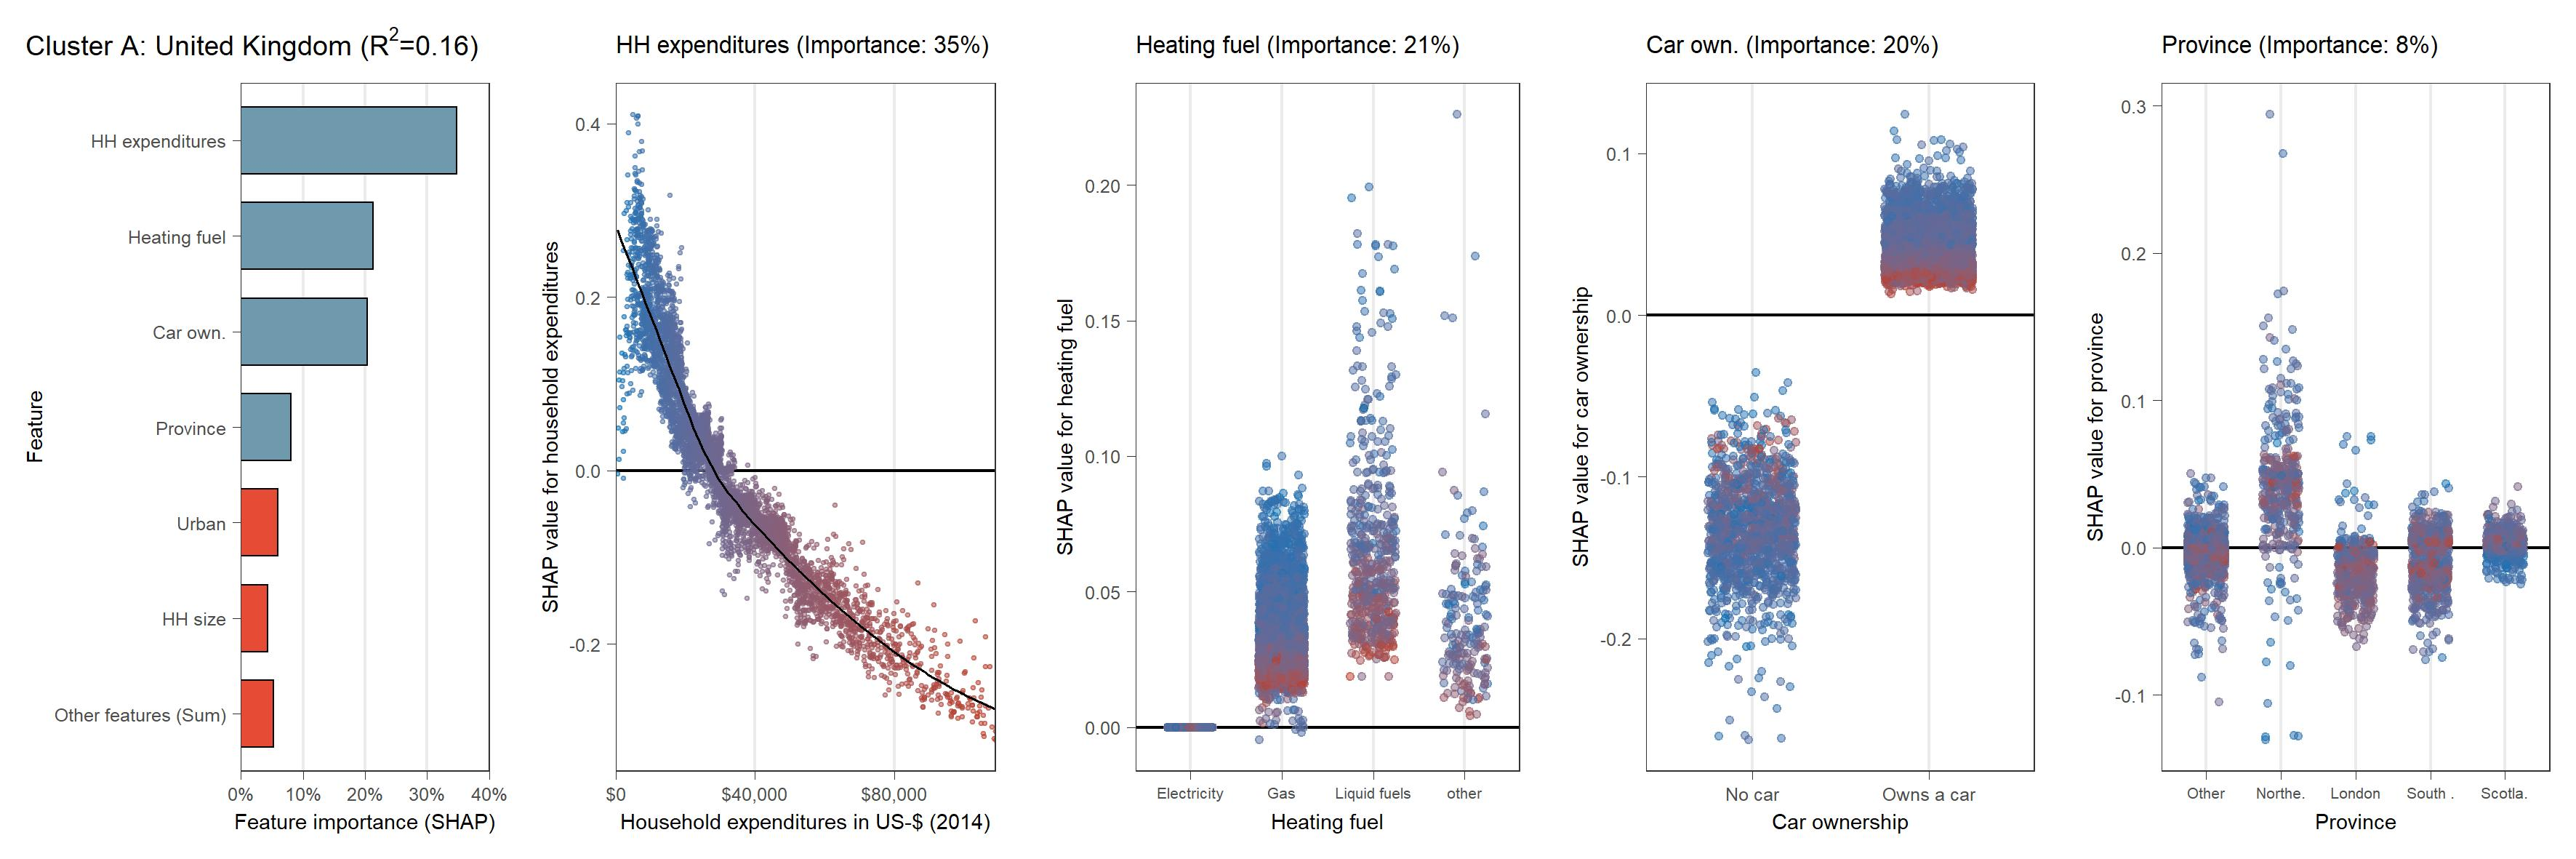
\includegraphics[width=\textwidth]{Figure_5b_GBR}
    \end{subfigure}
    \\
    \vspace{0.5cm}
    \begin{subcaption2}
     This figure shows SHAP-values for predicting carbon intensity over feature values for 87 countries in order of nine country-clusters. The bar chart displays normalized average absolute SHAP-values for all features. Features with less than 3\% of normalized SHAP-values are subsumed as "Other features (Sum)". Charts show SHAP-values over total household expenditures for all countries and for the three most important features in each country besides total household expenditures. Colors represent household expenditures with blue (red) colors indicating lower (higher) household expenditures.
     \end{subcaption2}
\end{figure}

\begin{figure}[ht!]\ContinuedFloat
    \centering
   \begin{subfigure}[b]{\textwidth}
         \centering
         \caption{Partial dependence plot (SHAP) for Cyprus}
         \label{fig:5b_CYP}
         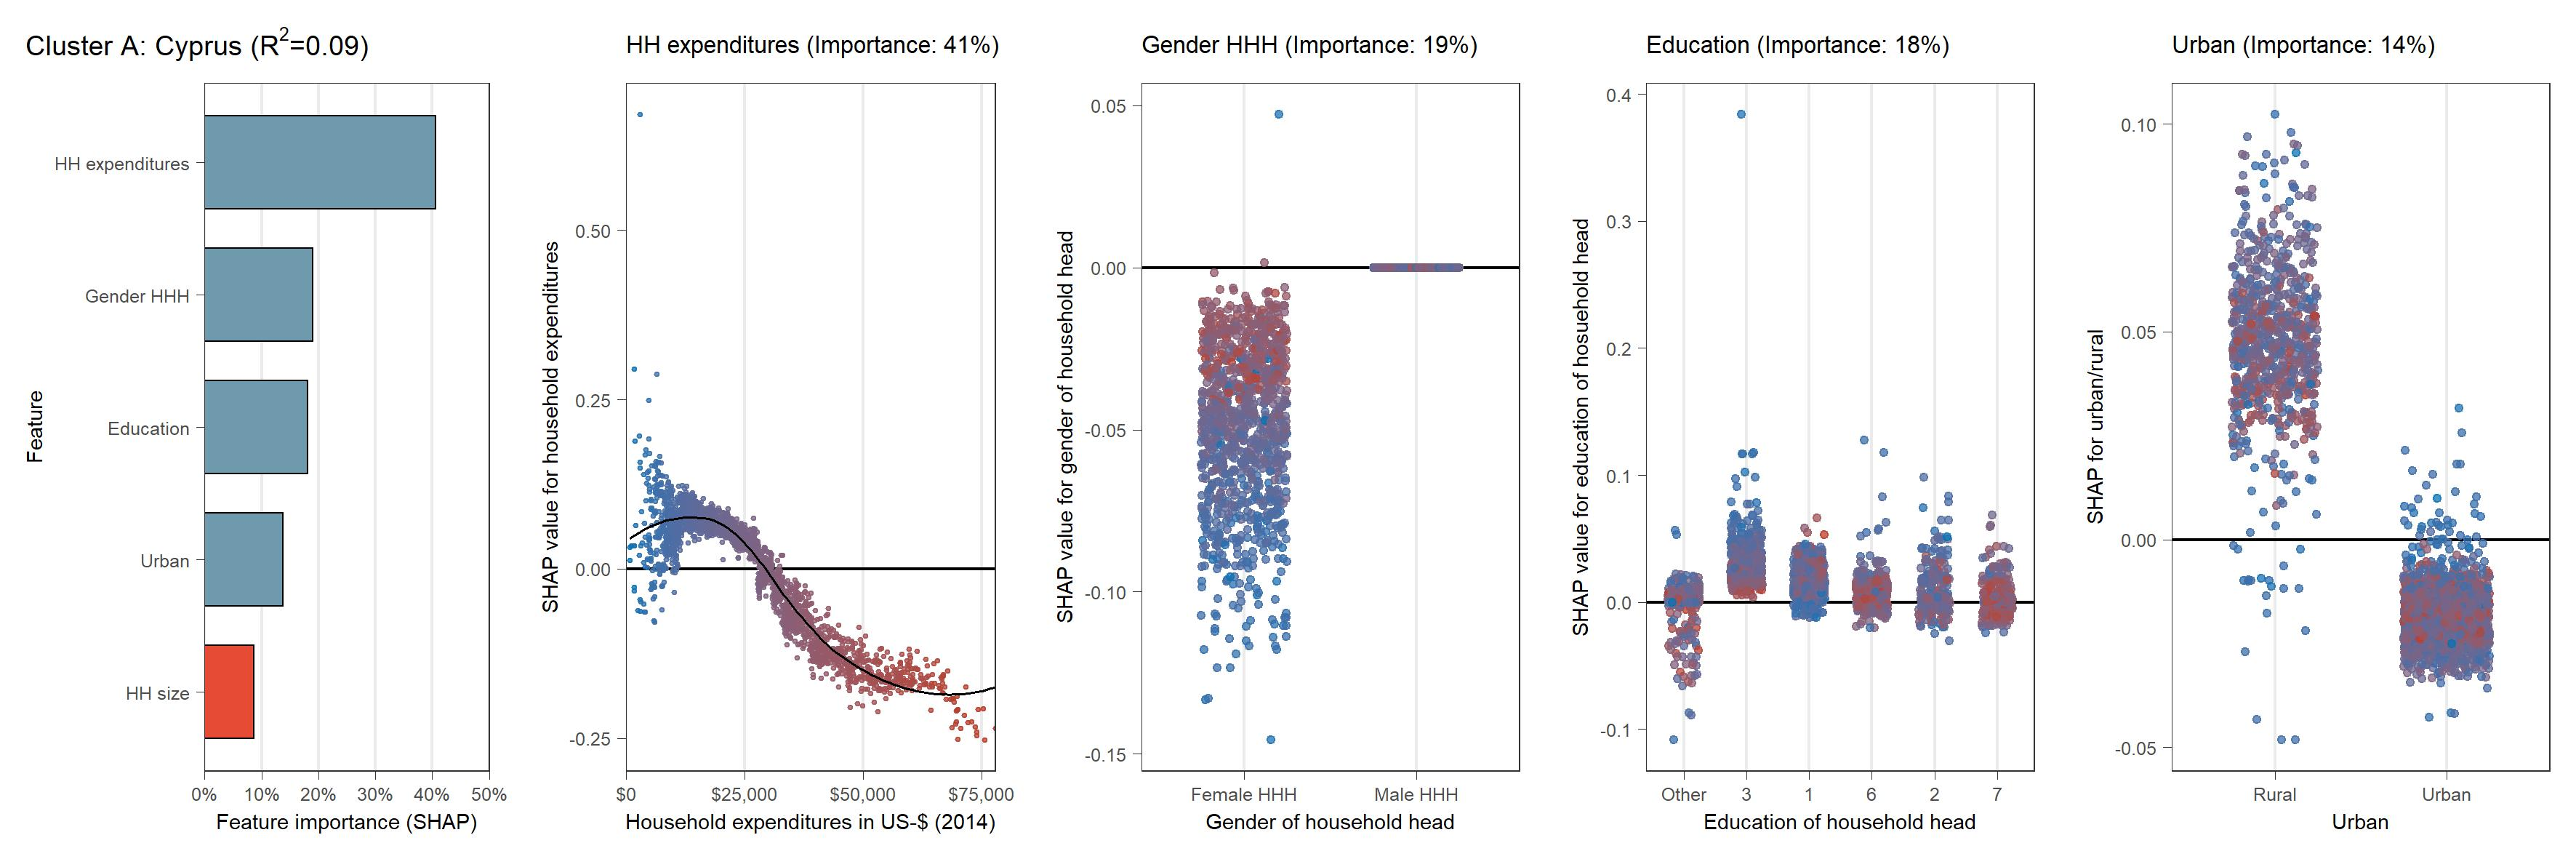
\includegraphics[width=\textwidth]{Figure_5b_CYP}         
     \end{subfigure}
    \\
    \vspace{0.5cm}
   \begin{subfigure}[b]{\textwidth}
         \centering
         \caption{Partial dependence plot (SHAP) for Maldives}
         \label{fig:5b_MDV}
         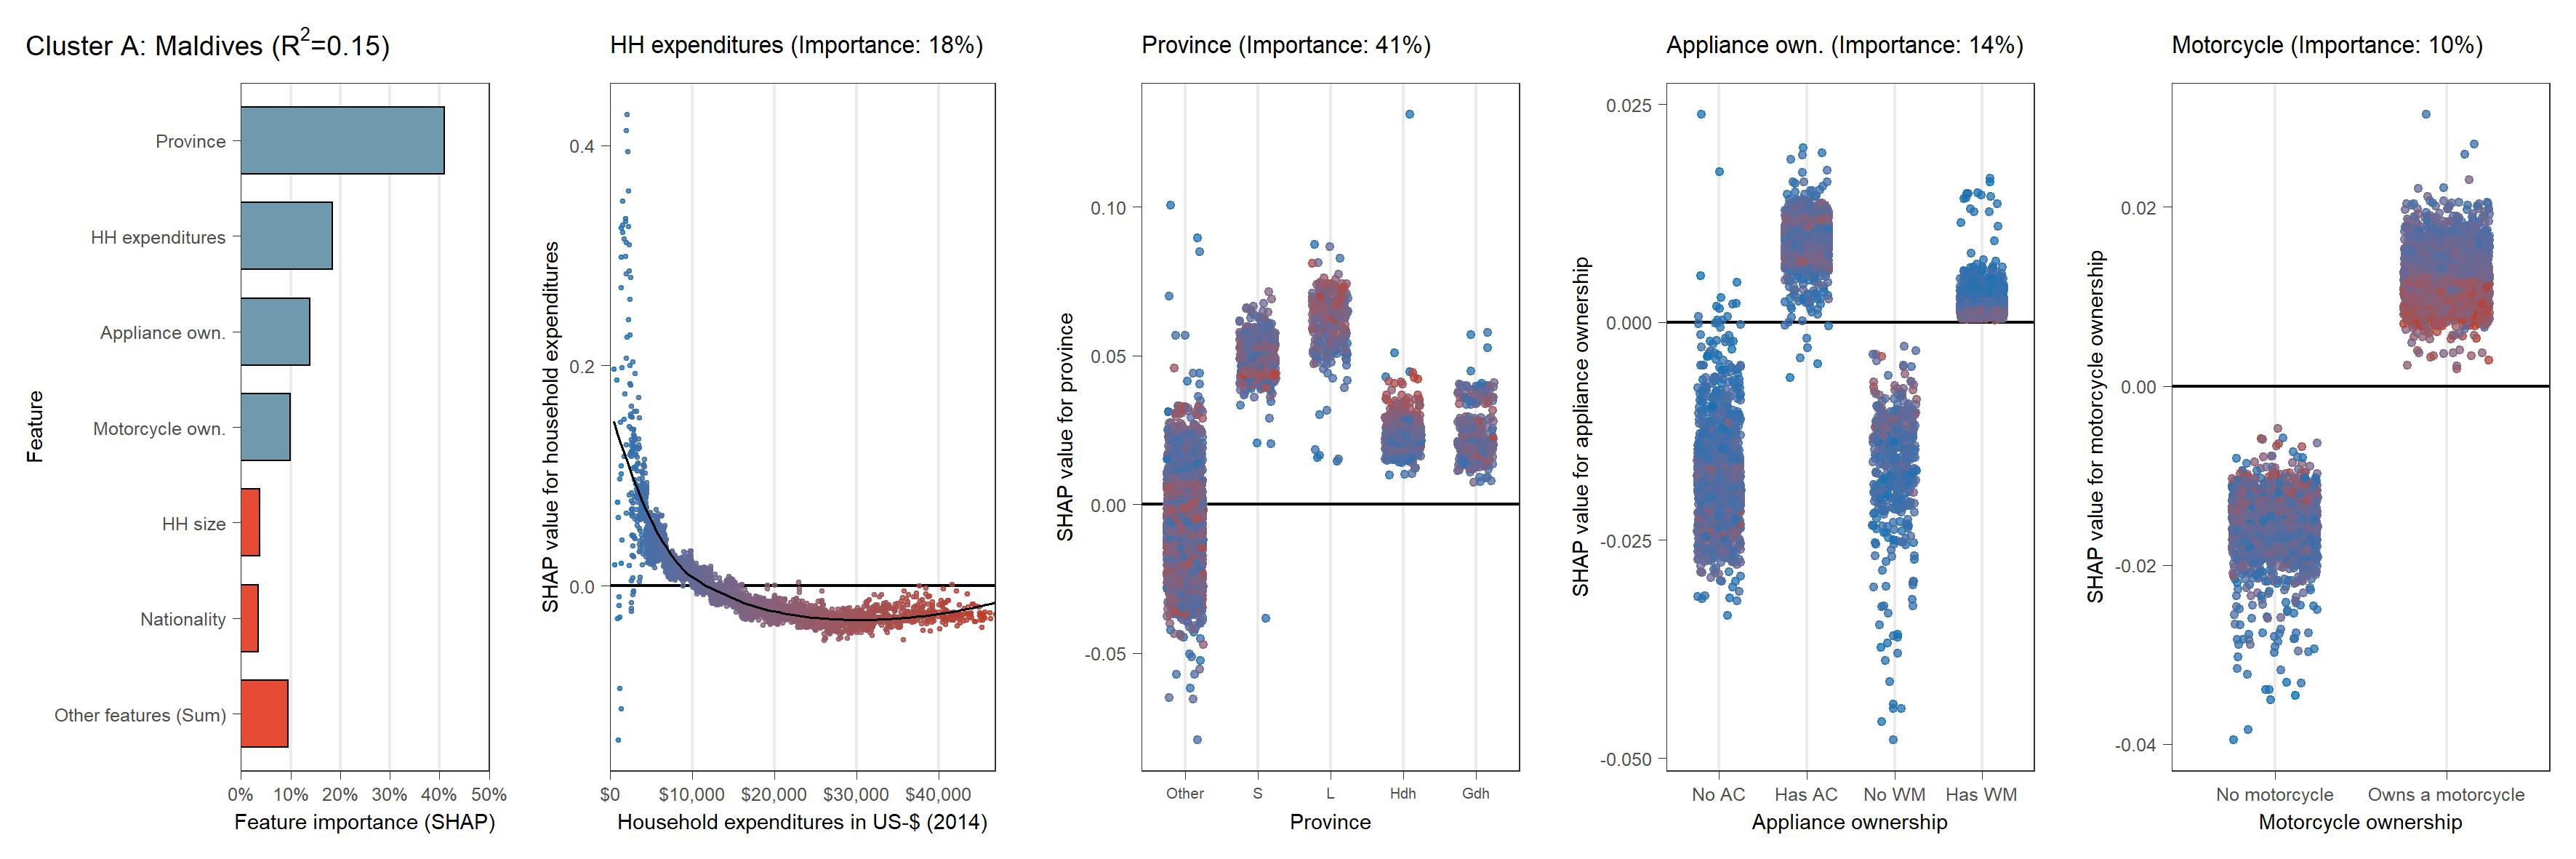
\includegraphics[width=\textwidth]{Figure_5b_MDV}         
     \end{subfigure}
    \\
    \vspace{0.5cm}
   \begin{subfigure}[b]{\textwidth}
         \centering
         \caption{Partial dependence plot (SHAP) for Germany}
         \label{fig:5b_DEU}
         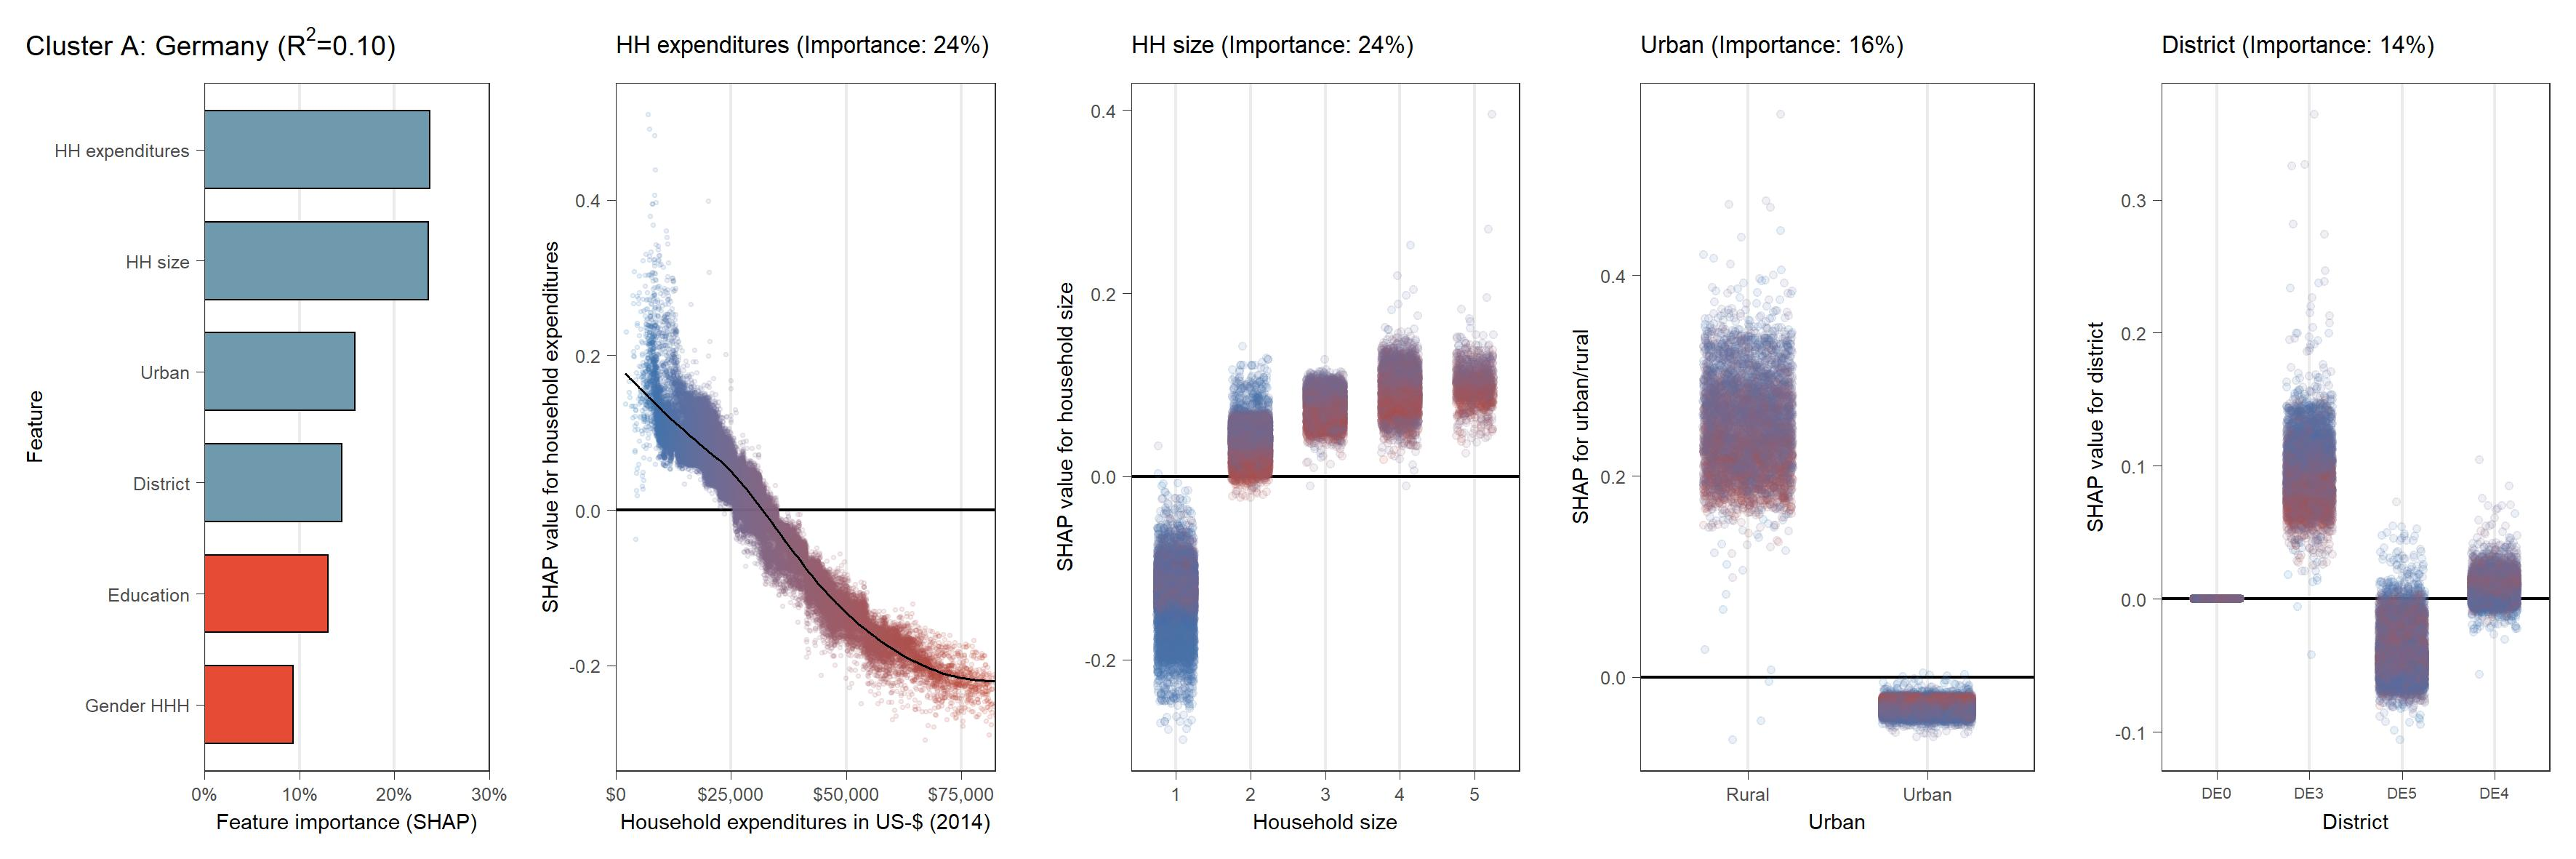
\includegraphics[width=\textwidth]{Figure_5b_DEU}
    \end{subfigure}
    \\
    \vspace{0.5cm}
    \begin{subcaption2}
     This figure shows SHAP-values for predicting carbon intensity over feature values for 87 countries in order of nine country-clusters. The bar chart displays normalized average absolute SHAP-values for all features. Features with less than 3\% of normalized SHAP-values are subsumed as "Other features (Sum)". Charts show SHAP-values over total household expenditures for all countries and for the three most important features in each country besides total household expenditures. Colors represent household expenditures with blue (red) colors indicating lower (higher) household expenditures.
     \end{subcaption2}
\end{figure}

\begin{figure}[ht!]\ContinuedFloat
    \centering
   \begin{subfigure}[b]{\textwidth}
         \centering
         \caption{Partial dependence plot (SHAP) for Canada}
         \label{fig:5b_CAN}
         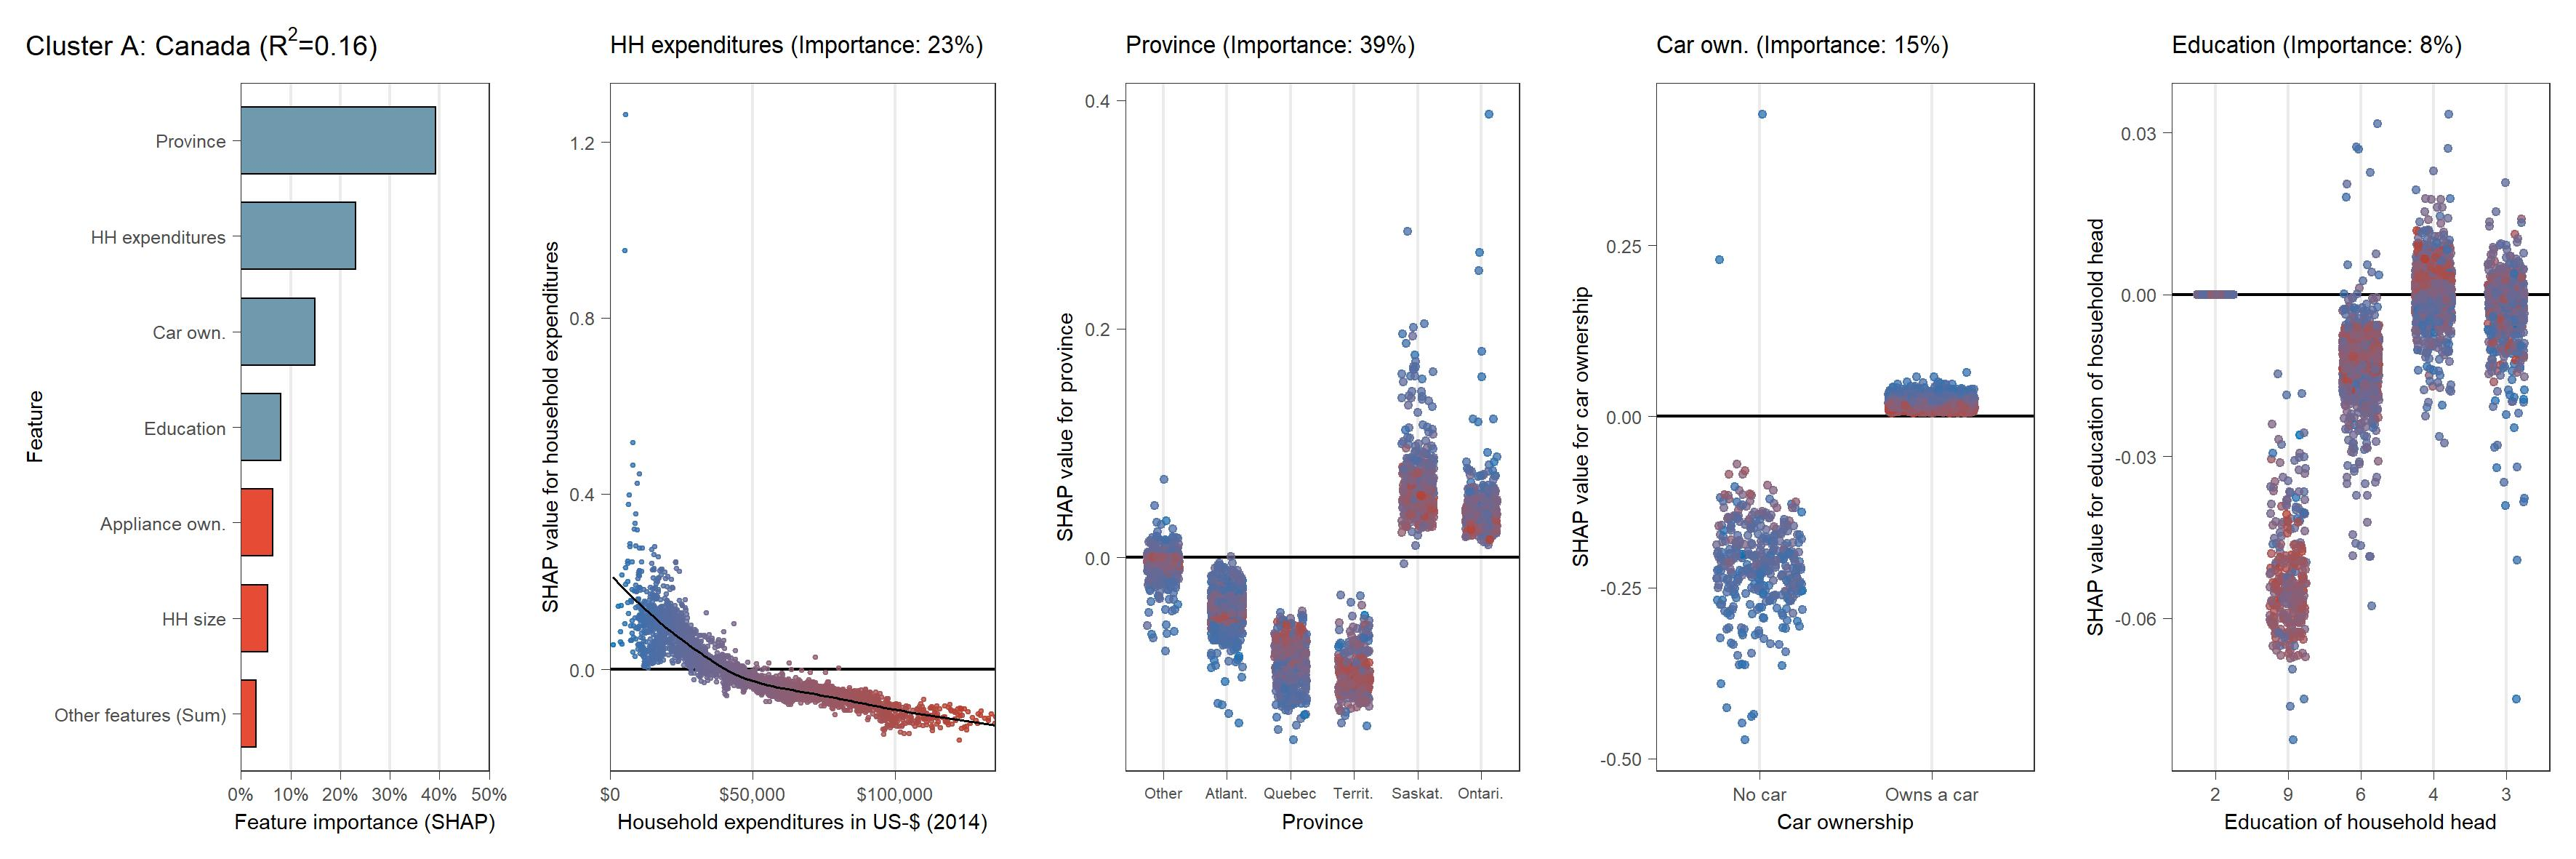
\includegraphics[width=\textwidth]{Figure_5b_CAN}         
     \end{subfigure}
    \\
    \vspace{0.5cm}
   \begin{subfigure}[b]{\textwidth}
         \centering
         \caption{Partial dependence plot (SHAP) for the Netherlands}
         \label{fig:5b_NLD}
         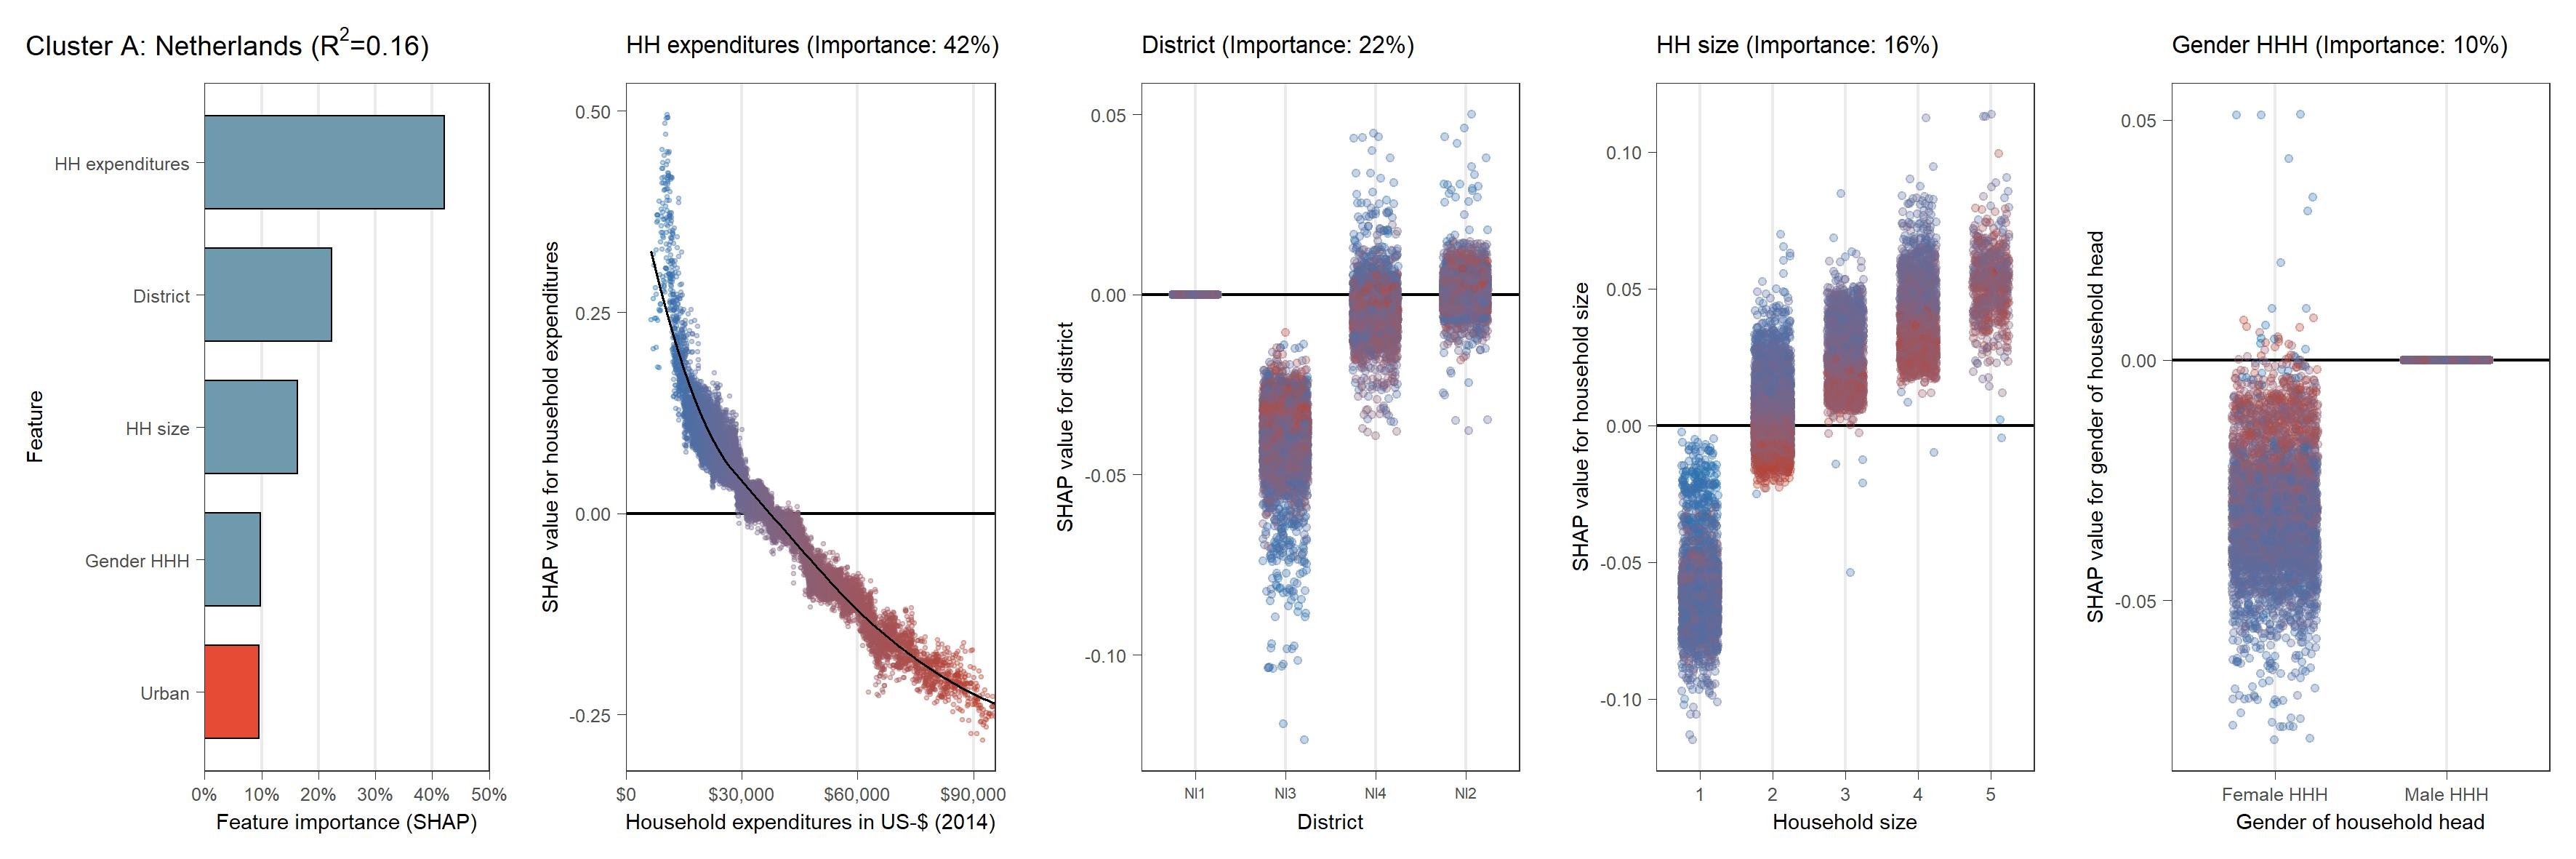
\includegraphics[width=\textwidth]{Figure_5b_NLD}         
     \end{subfigure}
    \\
    \vspace{0.5cm}
   \begin{subfigure}[b]{\textwidth}
         \centering
         \caption{Partial dependence plot (SHAP) for Uruguay}
         \label{fig:5b_URY}
         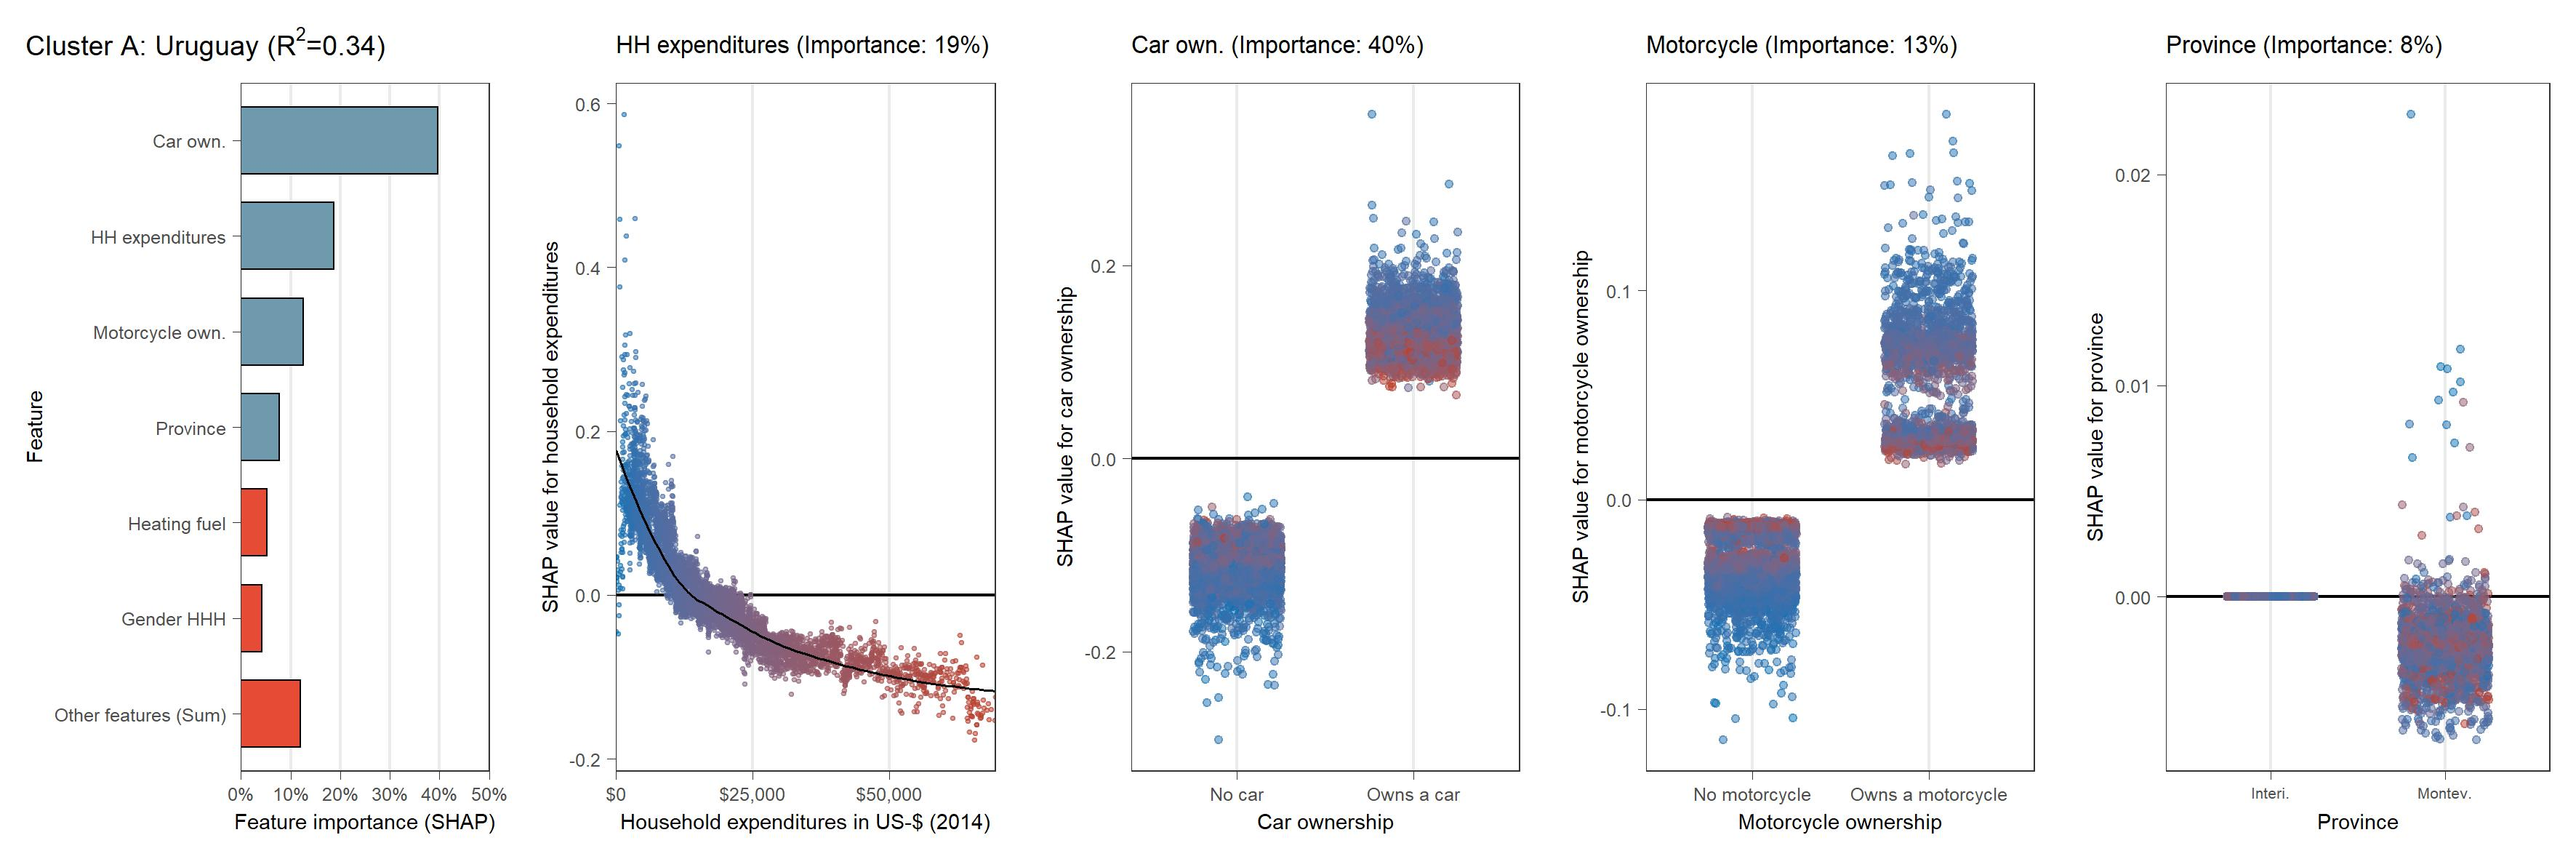
\includegraphics[width=\textwidth]{Figure_5b_URY}
    \end{subfigure}
    \\
    \vspace{0.5cm}
    \begin{subcaption2}
     This figure shows SHAP-values for predicting carbon intensity over feature values for 87 countries in order of nine country-clusters. The bar chart displays normalized average absolute SHAP-values for all features. Features with less than 3\% of normalized SHAP-values are subsumed as "Other features (Sum)". Charts show SHAP-values over total household expenditures for all countries and for the three most important features in each country besides total household expenditures. Colors represent household expenditures with blue (red) colors indicating lower (higher) household expenditures.
     \end{subcaption2}
\end{figure}

\begin{figure}[ht!]\ContinuedFloat
    \centering
   \begin{subfigure}[b]{\textwidth}
         \centering
         \caption{Partial dependence plot (SHAP) for Mongolia}
         \label{fig:5b_MNG}
         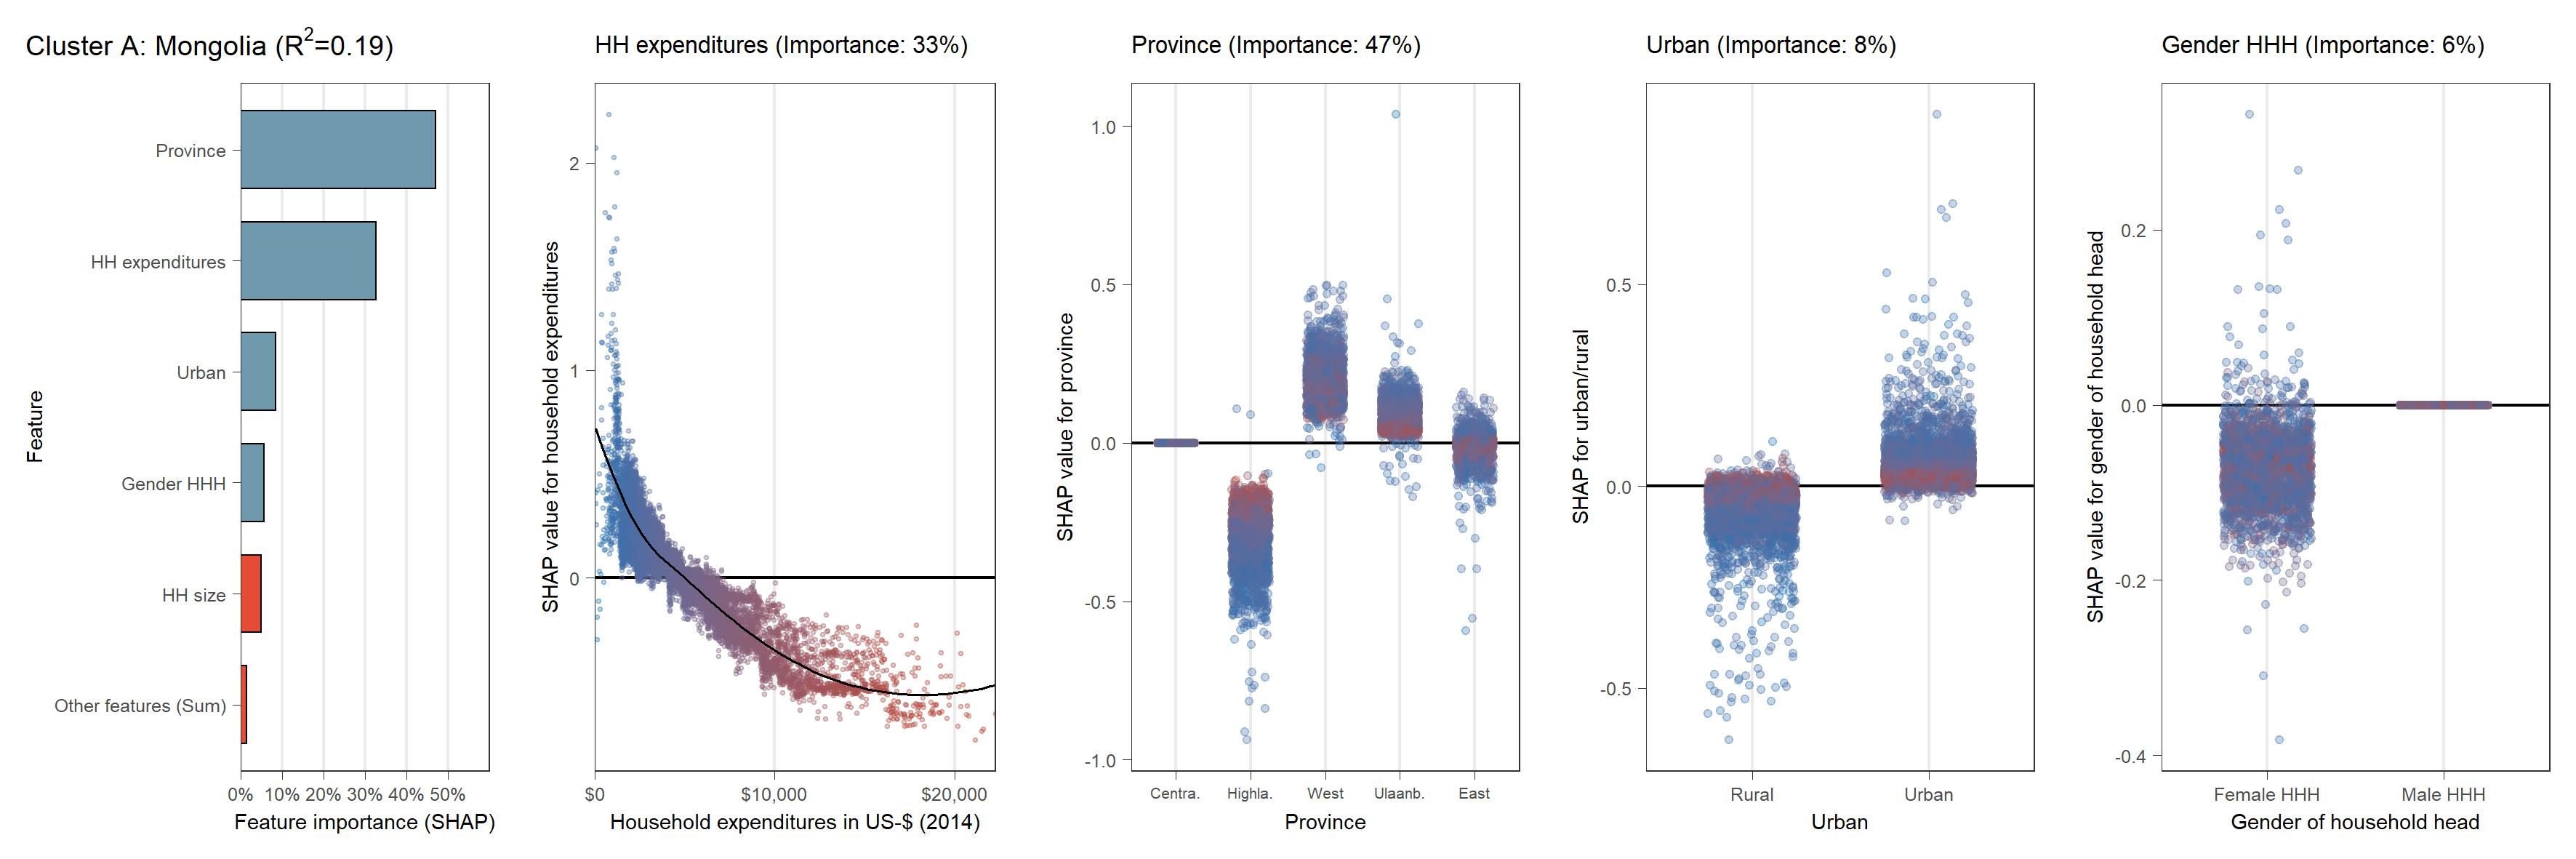
\includegraphics[width=\textwidth]{Figure_5b_MNG}         
     \end{subfigure}
    \\
    \vspace{0.5cm}
   \begin{subfigure}[b]{\textwidth}
         \centering
         \caption{Partial dependence plot (SHAP) for Barbados}
         \label{fig:5b_BRB}
         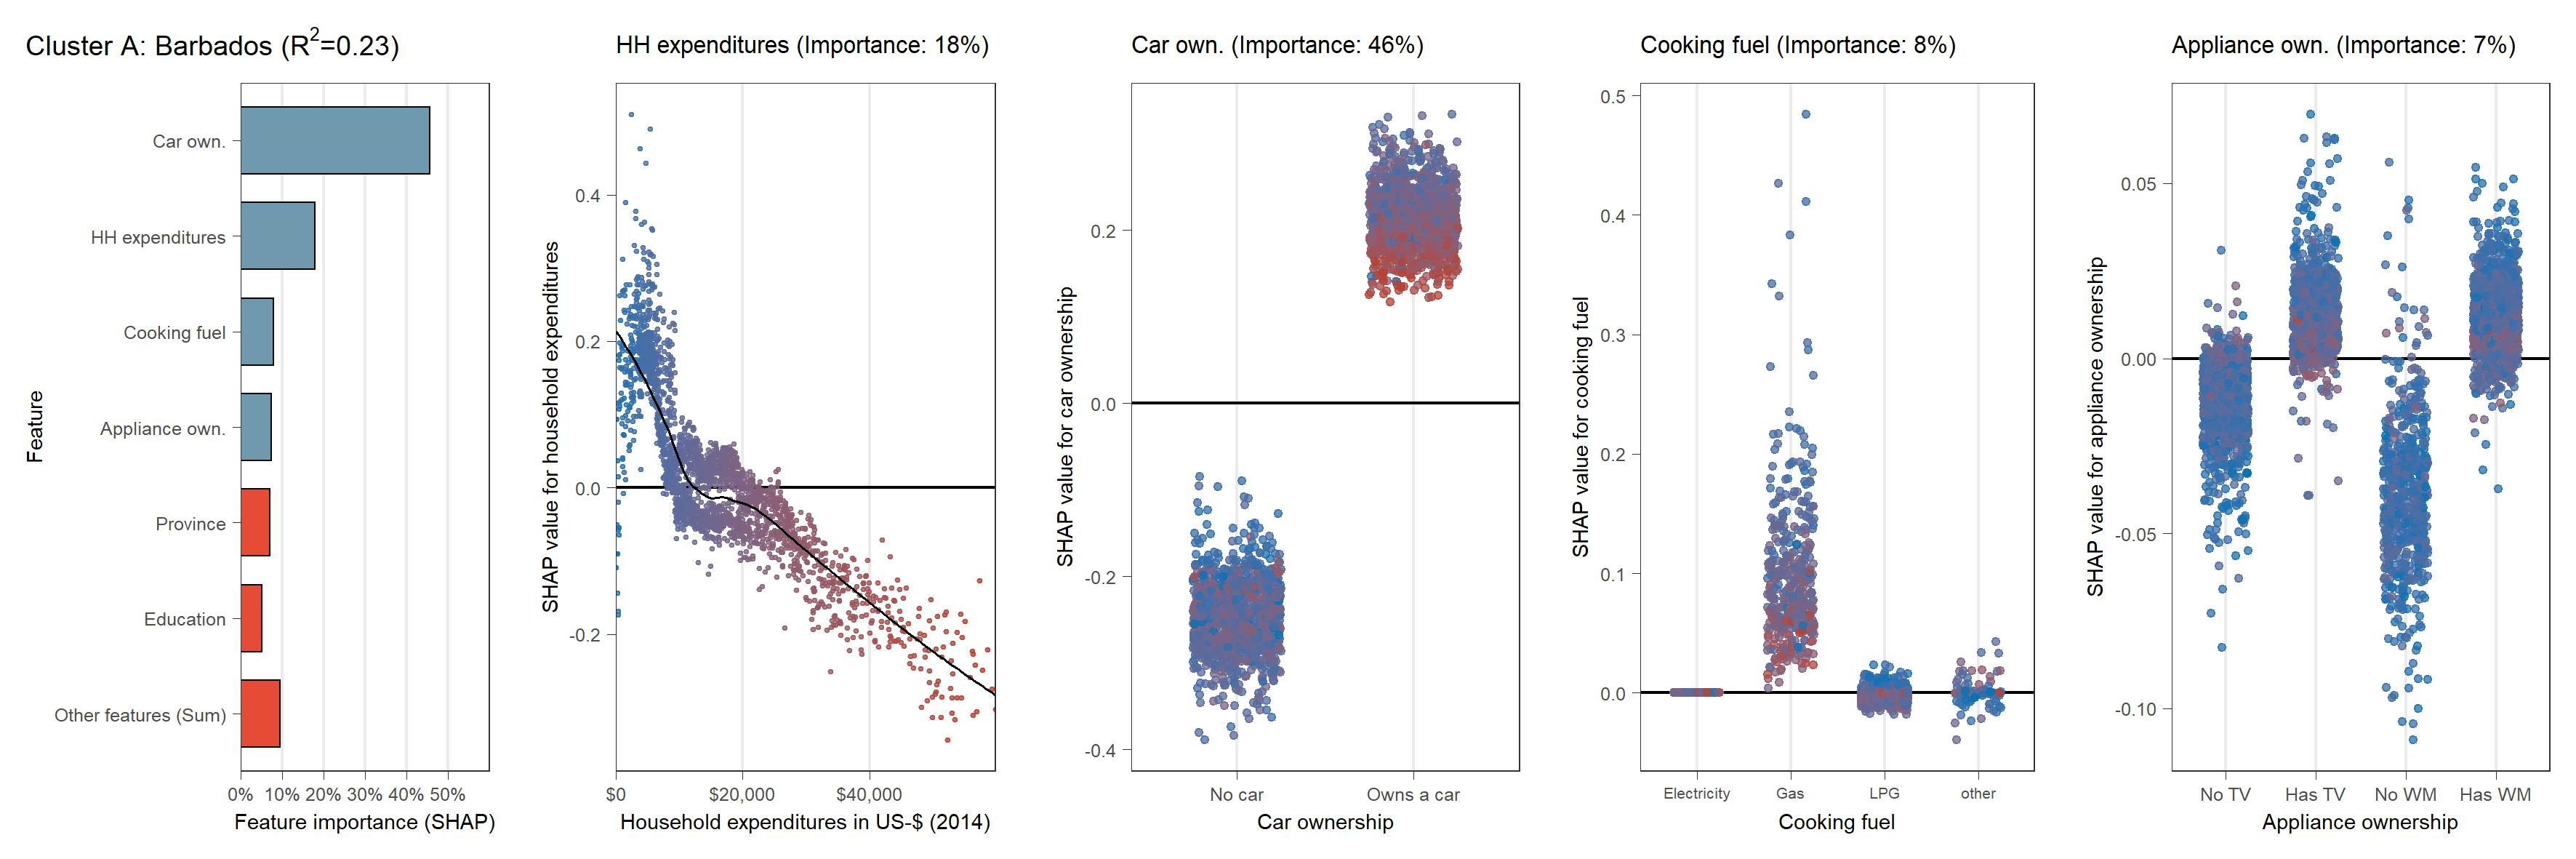
\includegraphics[width=\textwidth]{Figure_5b_BRB}         
     \end{subfigure}
    \\
    \vspace{0.5cm}
   \begin{subfigure}[b]{\textwidth}
         \centering
         \caption{Partial dependence plot (SHAP) for Argentina}
         \label{fig:5b_ARG}
         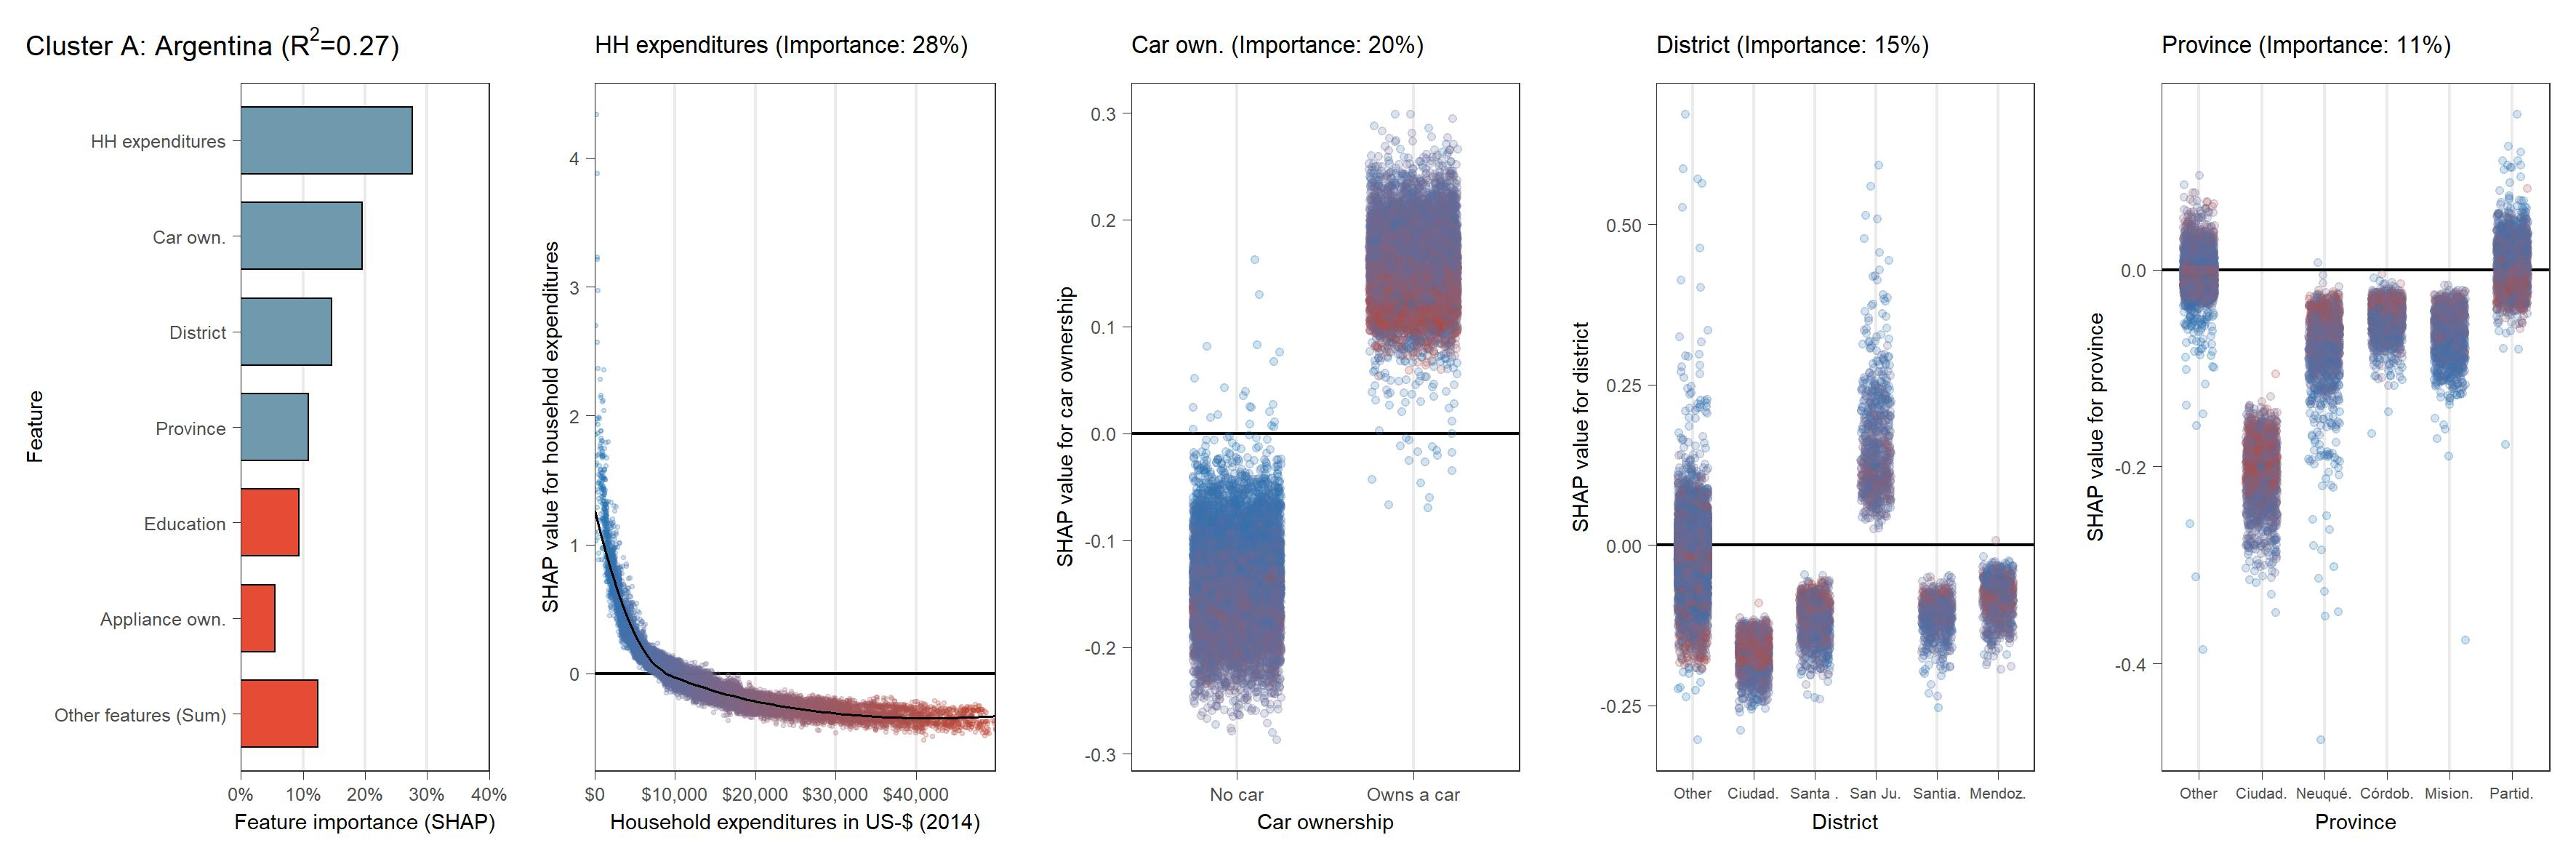
\includegraphics[width=\textwidth]{Figure_5b_ARG}
    \end{subfigure}
    \\
    \vspace{0.5cm}
    \begin{subcaption2}
     This figure shows SHAP-values for predicting carbon intensity over feature values for 87 countries in order of nine country-clusters. The bar chart displays normalized average absolute SHAP-values for all features. Features with less than 3\% of normalized SHAP-values are subsumed as "Other features (Sum)". Charts show SHAP-values over total household expenditures for all countries and for the three most important features in each country besides total household expenditures. Colors represent household expenditures with blue (red) colors indicating lower (higher) household expenditures.
     \end{subcaption2}
\end{figure}

\begin{figure}[ht!]\ContinuedFloat
    \centering
   \begin{subfigure}[b]{\textwidth}
         \centering
         \caption{Partial dependence plot (SHAP) for Costa Rica}
         \label{fig:5b_CRI}
         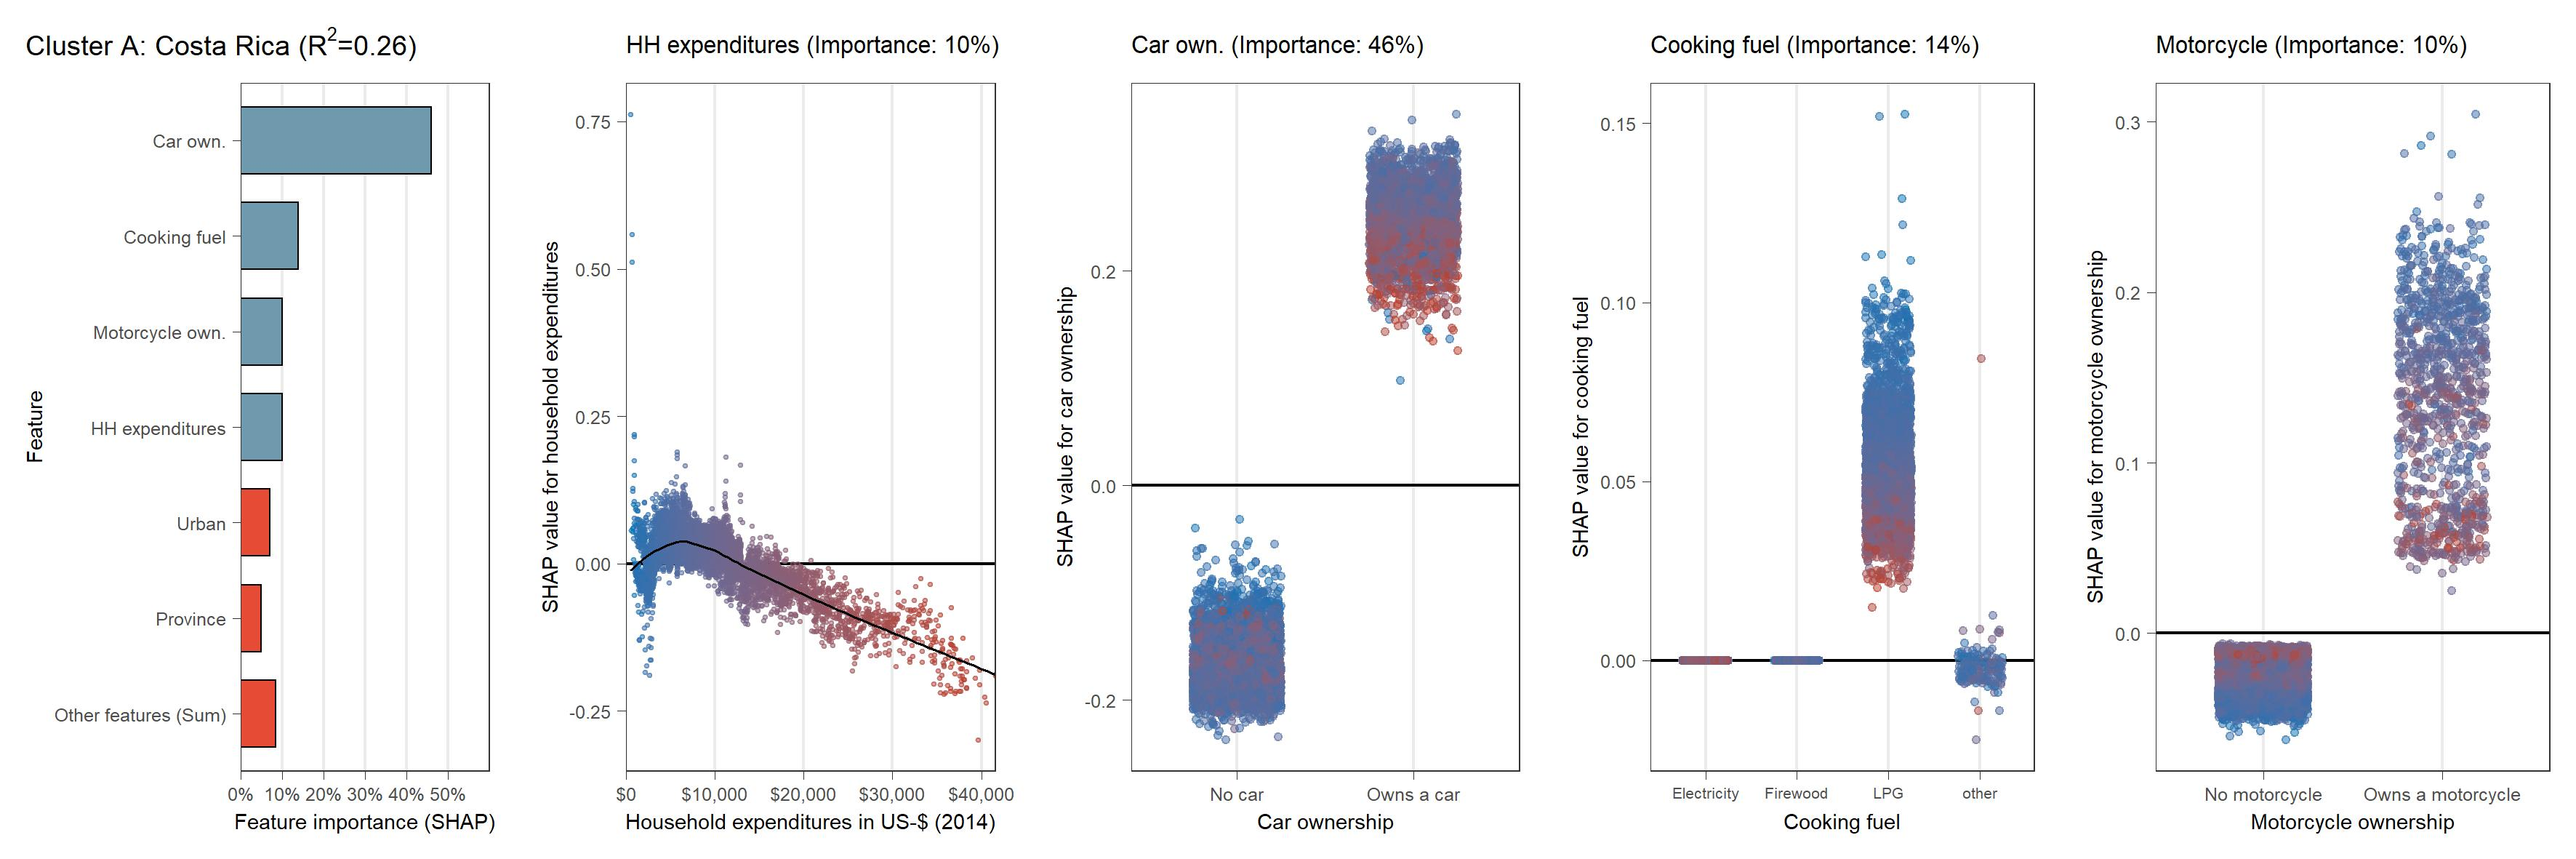
\includegraphics[width=\textwidth]{Figure_5b_CRI}         
     \end{subfigure}
    \\
    \vspace{0.5cm}
   \begin{subfigure}[b]{\textwidth}
         \centering
         \caption{Partial dependence plot (SHAP) for Italy}
         \label{fig:5b_ITA}
         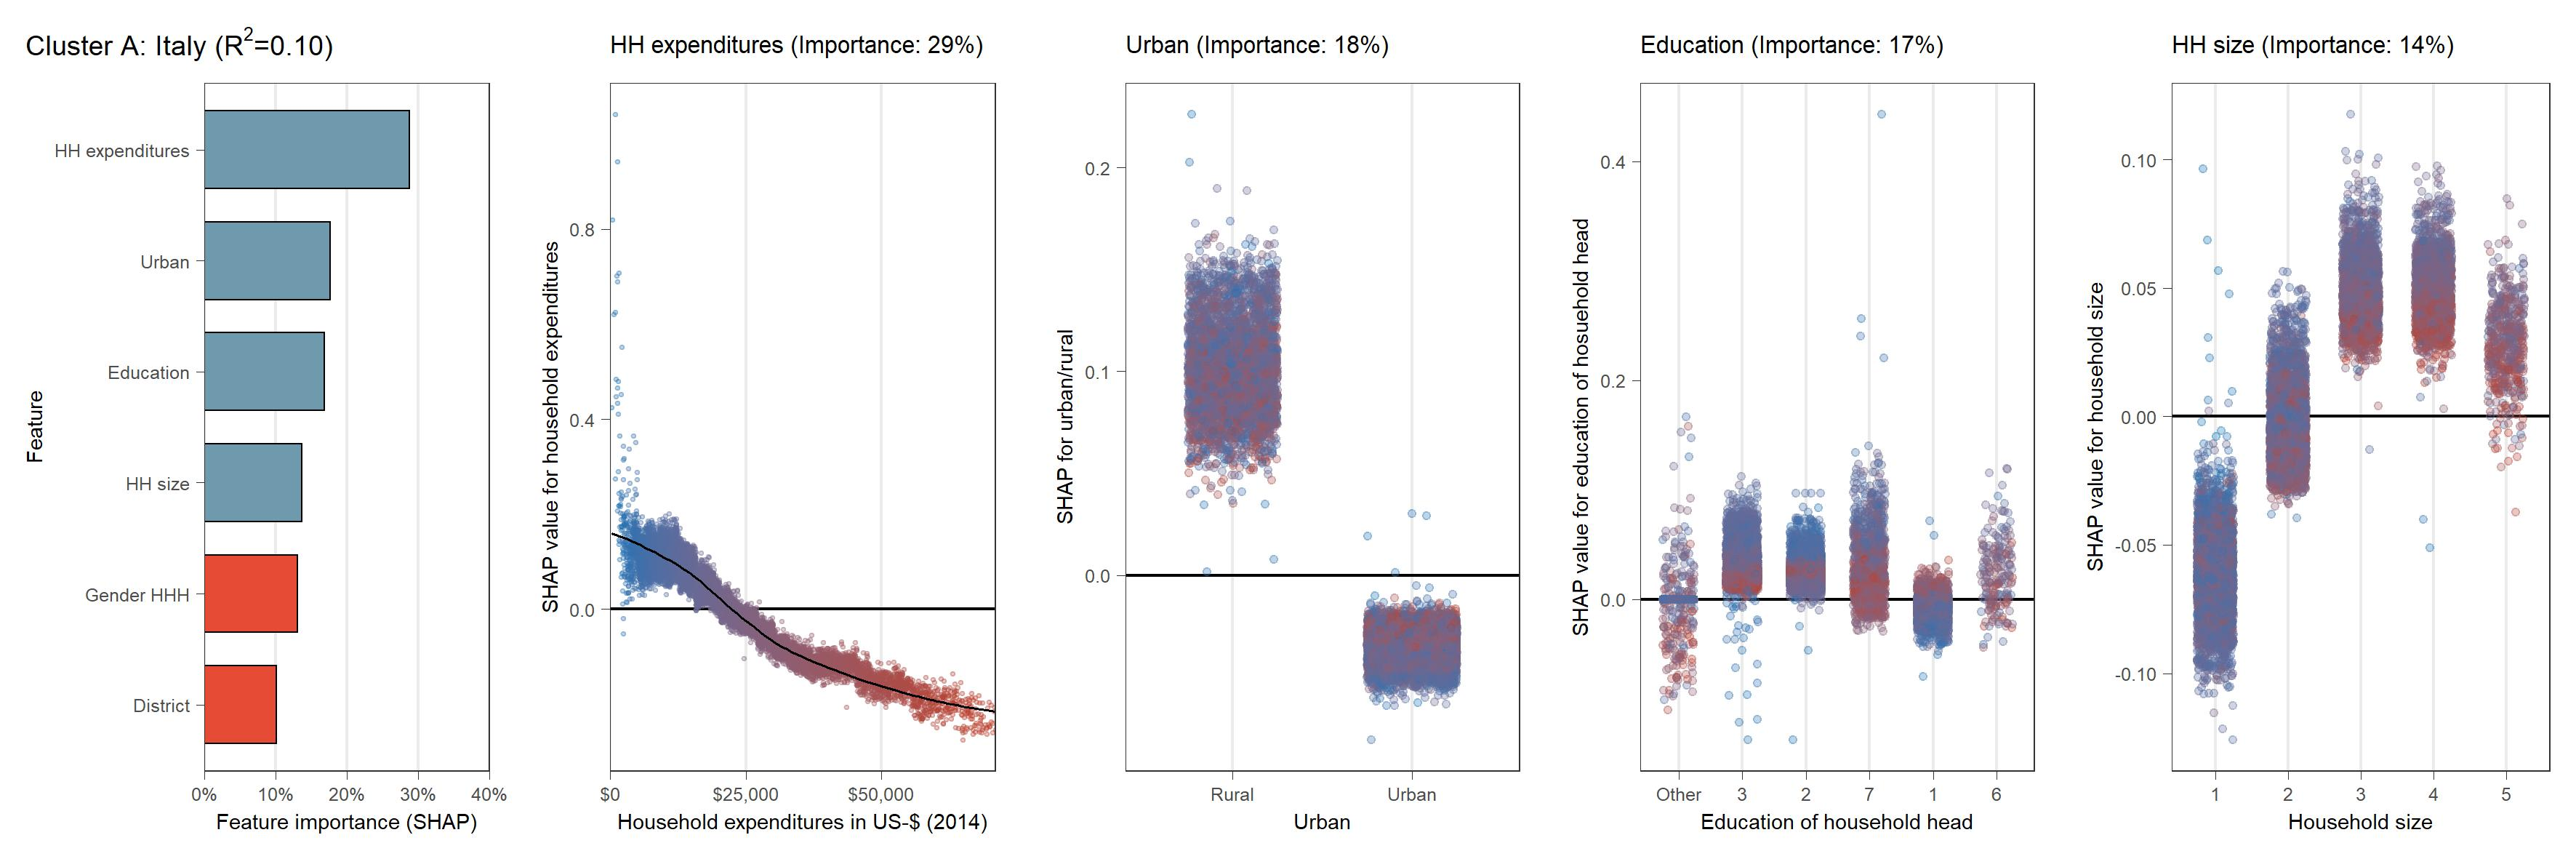
\includegraphics[width=\textwidth]{Figure_5b_ITA}         
     \end{subfigure}
    \\
    \vspace{0.5cm}
   \begin{subfigure}[b]{\textwidth}
         \centering
         \caption{Partial dependence plot (SHAP) for Israel}
         \label{fig:5b_ISR}
         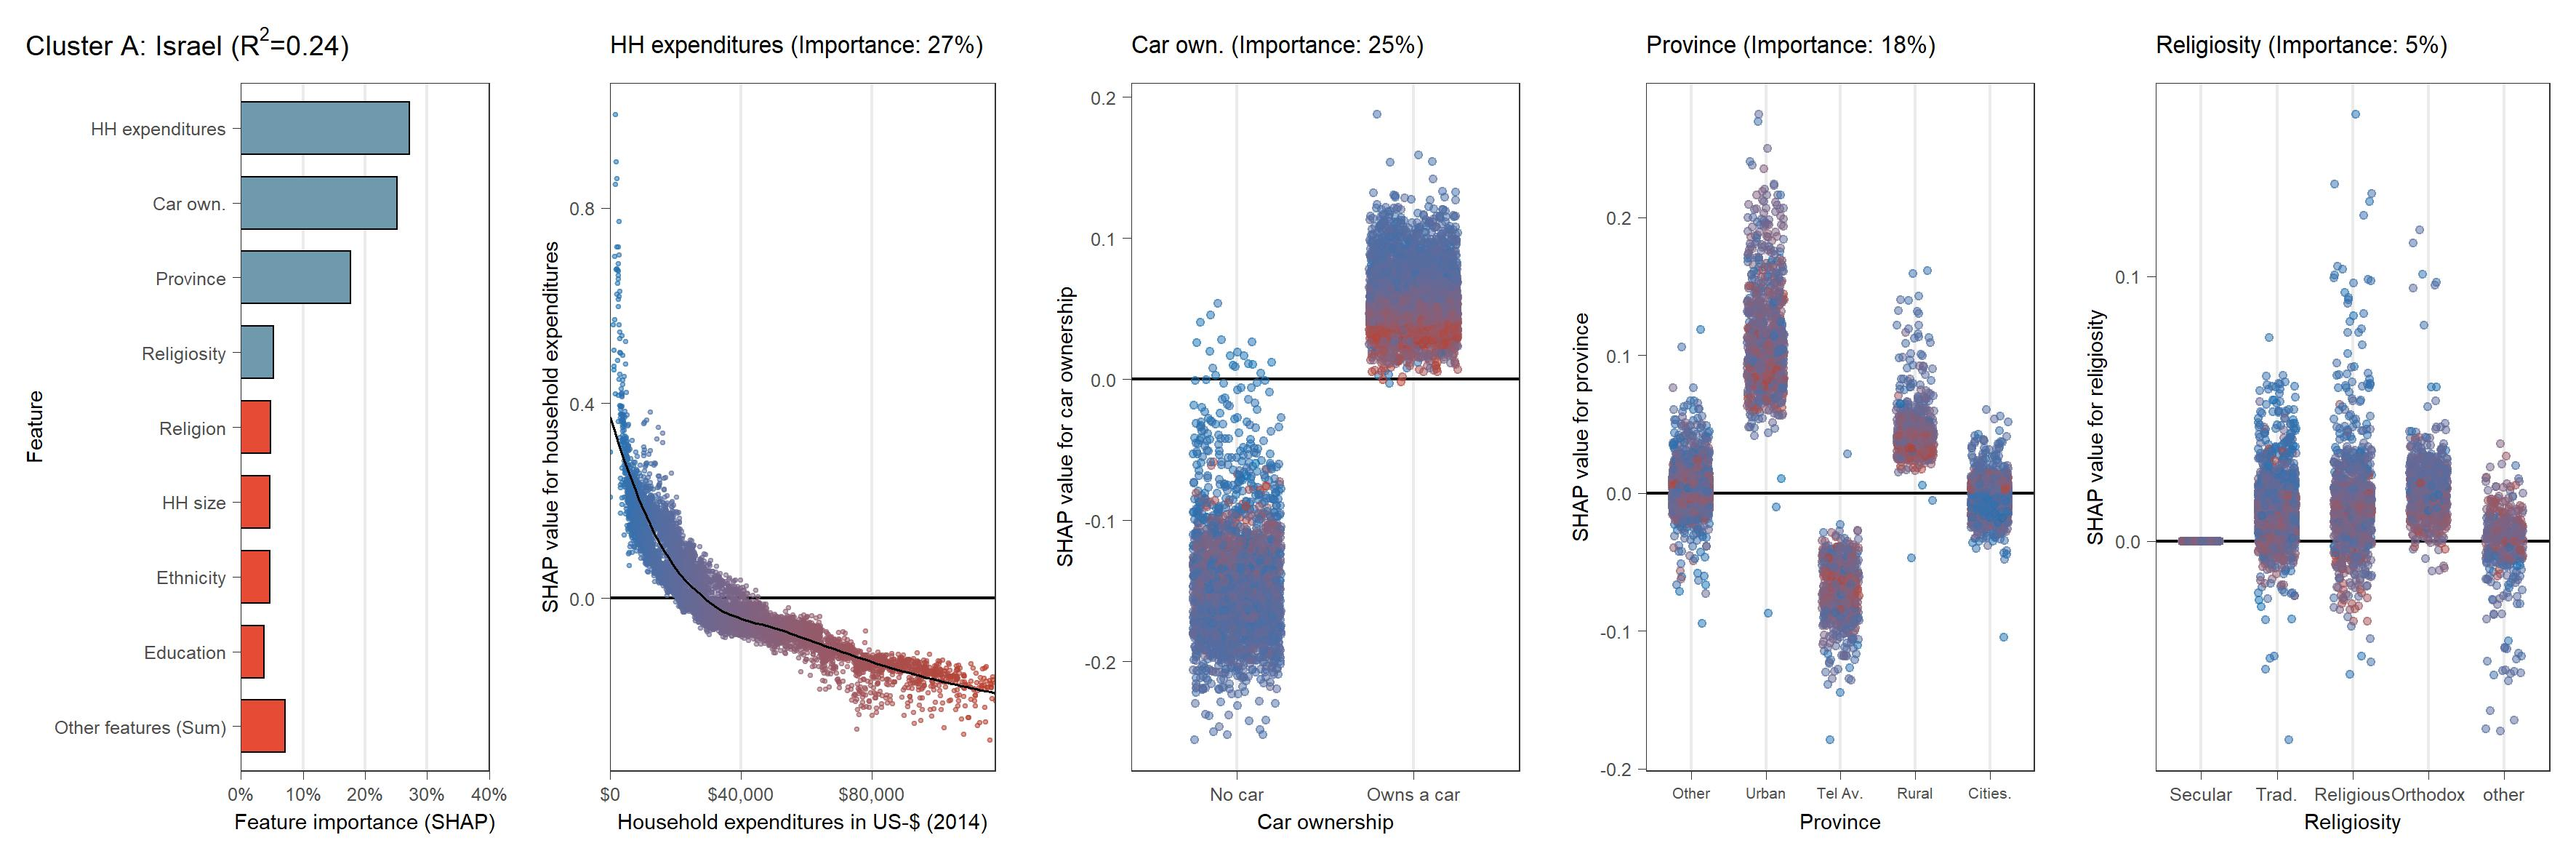
\includegraphics[width=\textwidth]{Figure_5b_ISR}
    \end{subfigure}
    \\
    \vspace{0.5cm}
    \begin{subcaption2}
     This figure shows SHAP-values for predicting carbon intensity over feature values for 87 countries in order of nine country-clusters. The bar chart displays normalized average absolute SHAP-values for all features. Features with less than 3\% of normalized SHAP-values are subsumed as "Other features (Sum)". Charts show SHAP-values over total household expenditures for all countries and for the three most important features in each country besides total household expenditures. Colors represent household expenditures with blue (red) colors indicating lower (higher) household expenditures.
     \end{subcaption2}
\end{figure}

\begin{figure}[ht!]\ContinuedFloat
    \centering
   \begin{subfigure}[b]{\textwidth}
         \centering
         \caption{Partial dependence plot (SHAP) for Senegal}
         \label{fig:5b_SEN}
         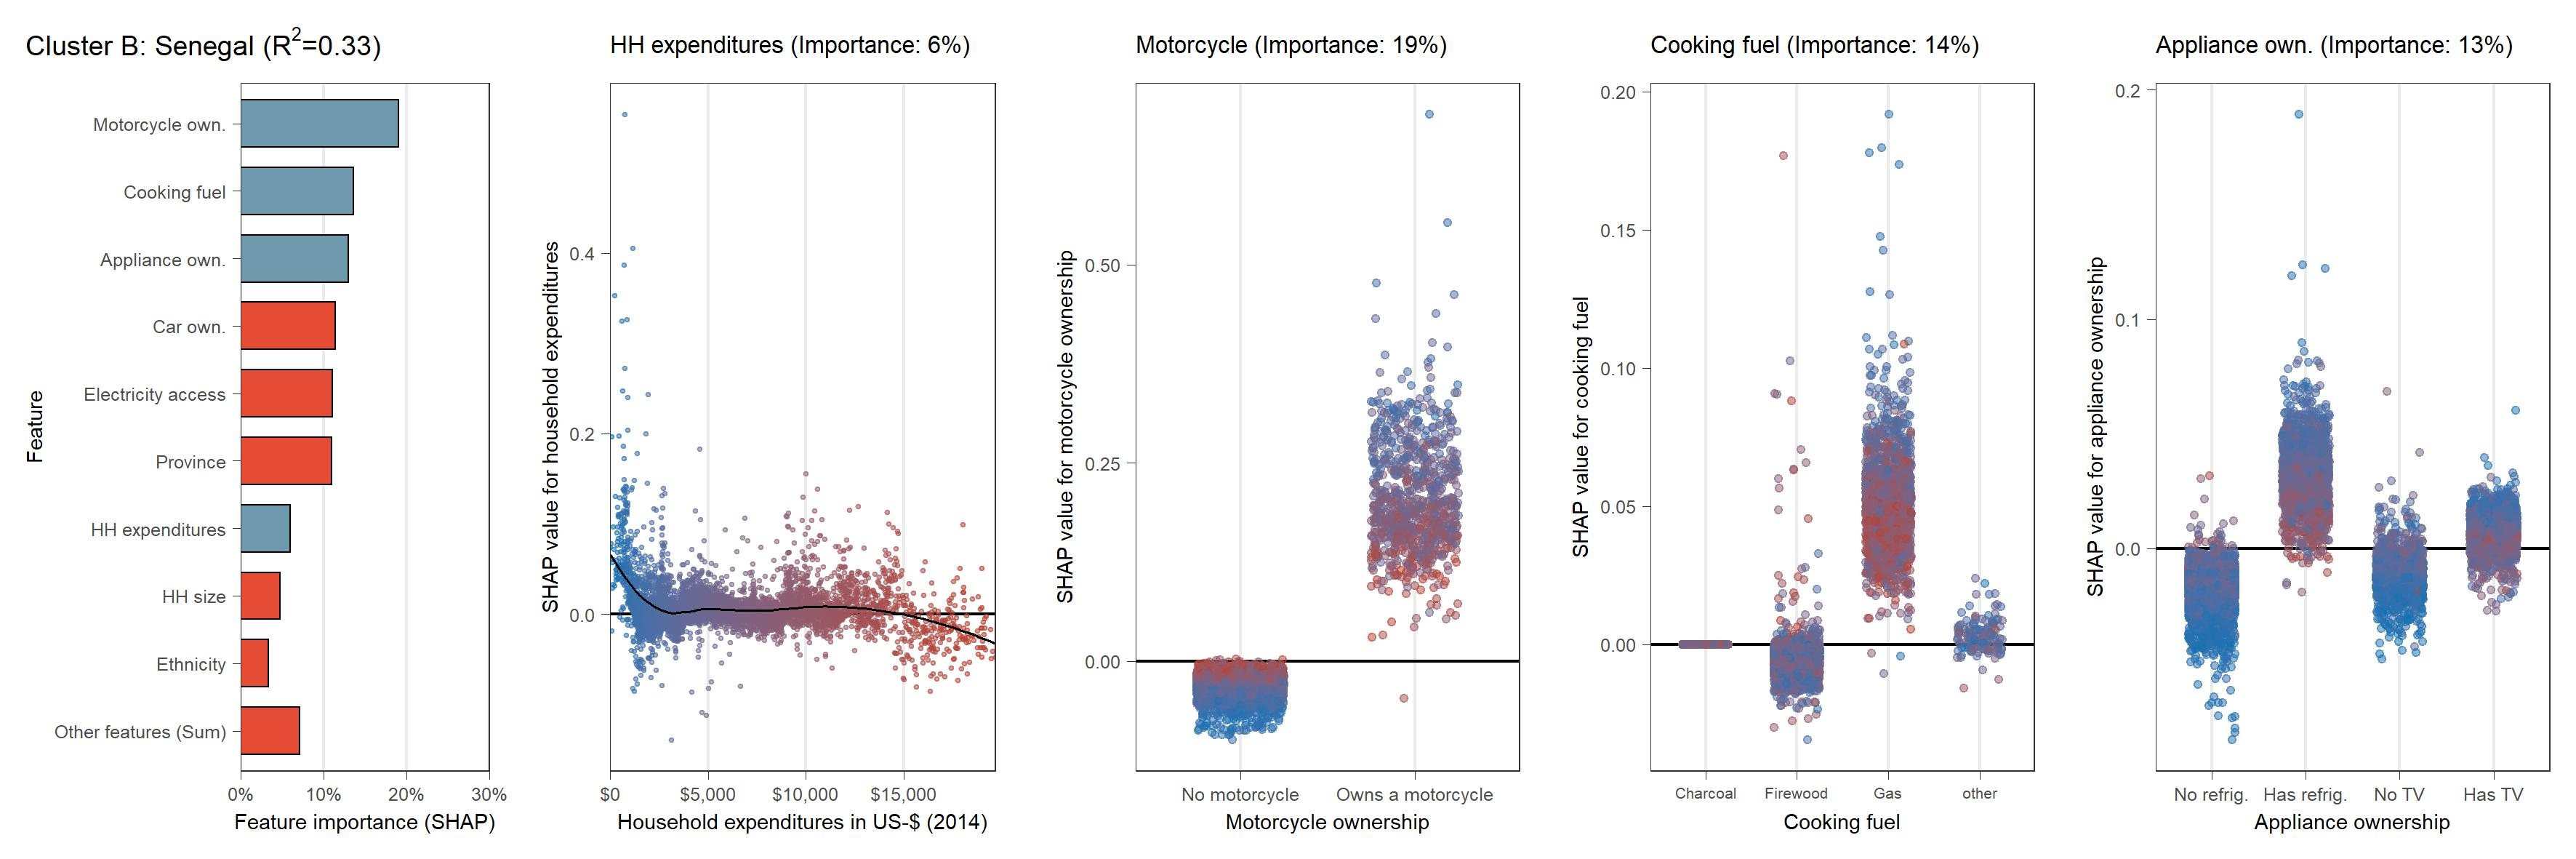
\includegraphics[width=\textwidth]{Figure_5b_SEN}         
     \end{subfigure}
    \\
    \vspace{0.5cm}
   \begin{subfigure}[b]{\textwidth}
         \centering
         \caption{Partial dependence plot (SHAP) for Ghana}
         \label{fig:5b_GHA}
         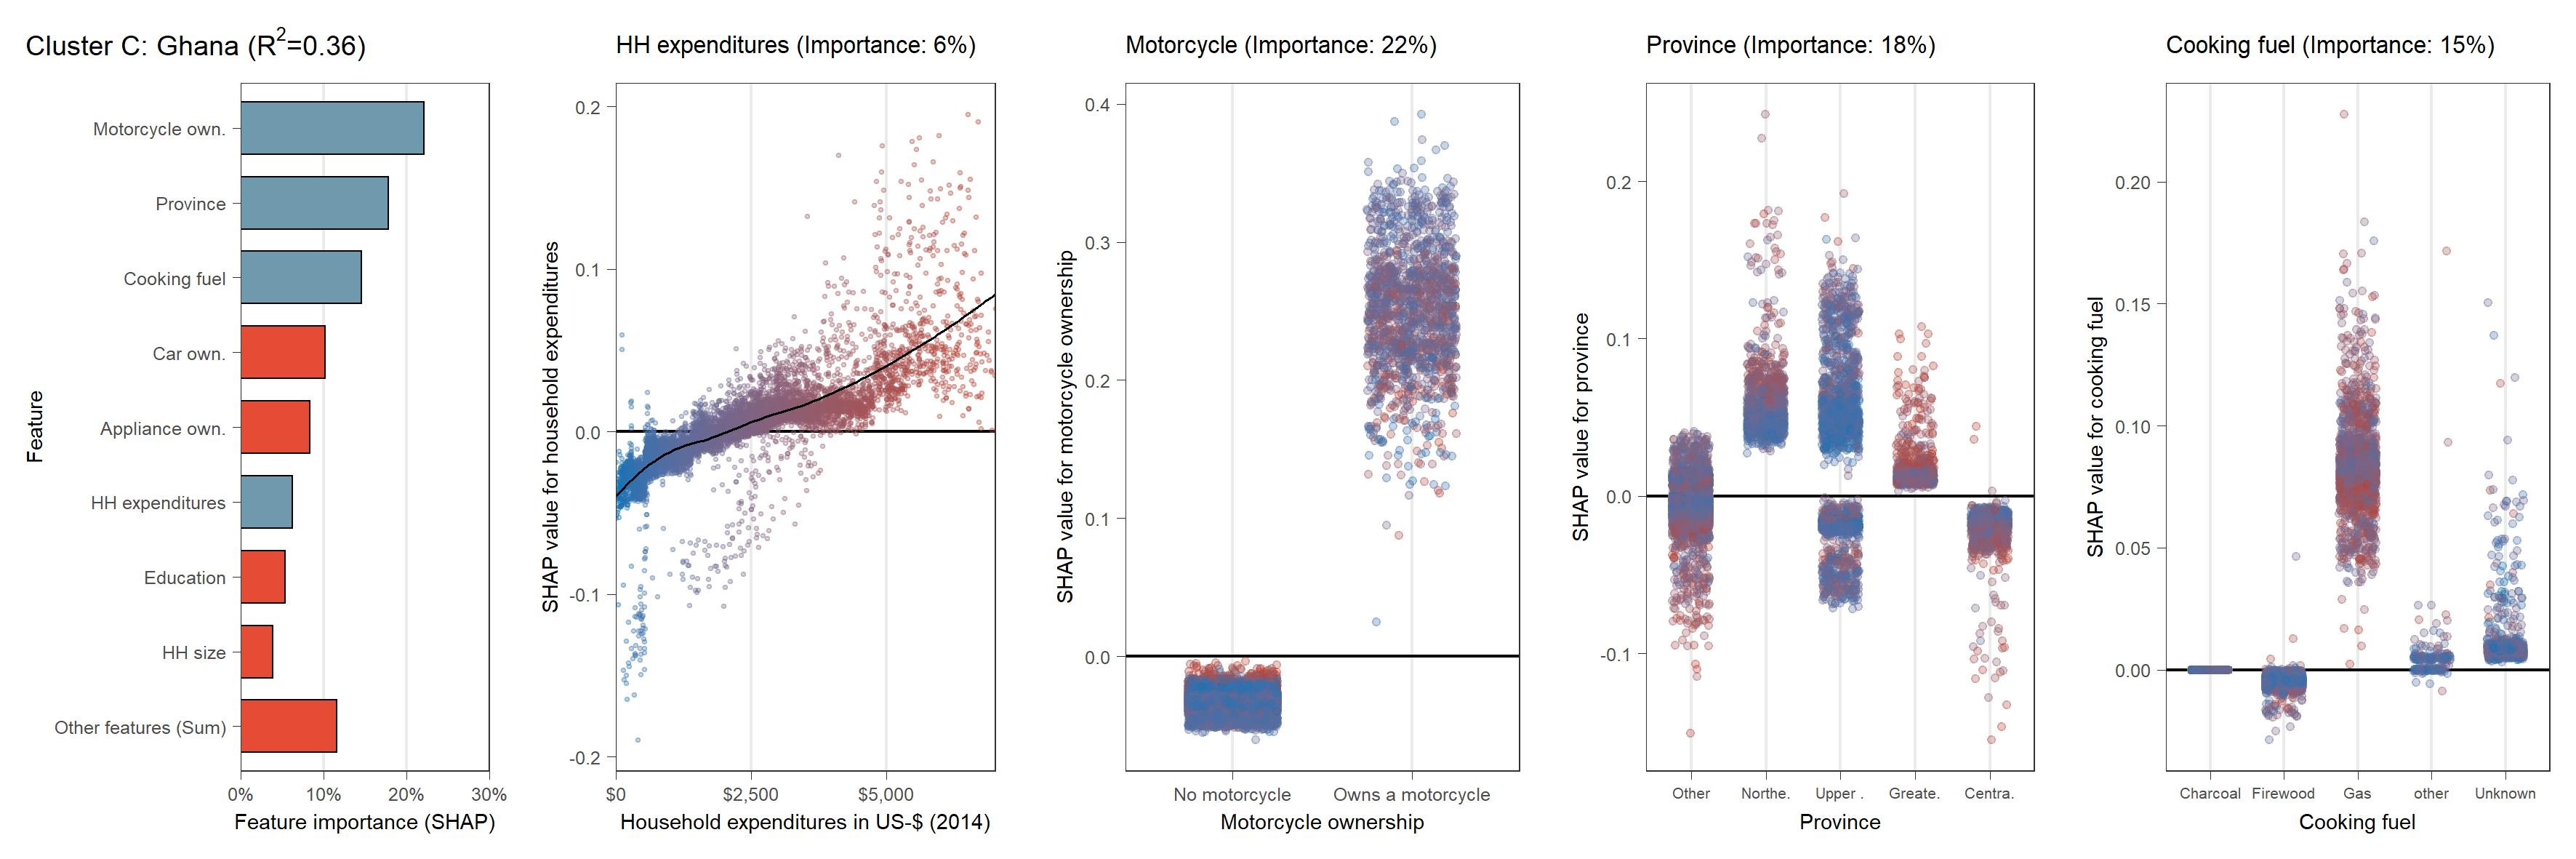
\includegraphics[width=\textwidth]{Figure_5b_GHA}         
     \end{subfigure}
    \\
    \vspace{0.5cm}
   \begin{subfigure}[b]{\textwidth}
         \centering
         \caption{Partial dependence plot (SHAP) for Nigeria}
         \label{fig:5b_NGA}
         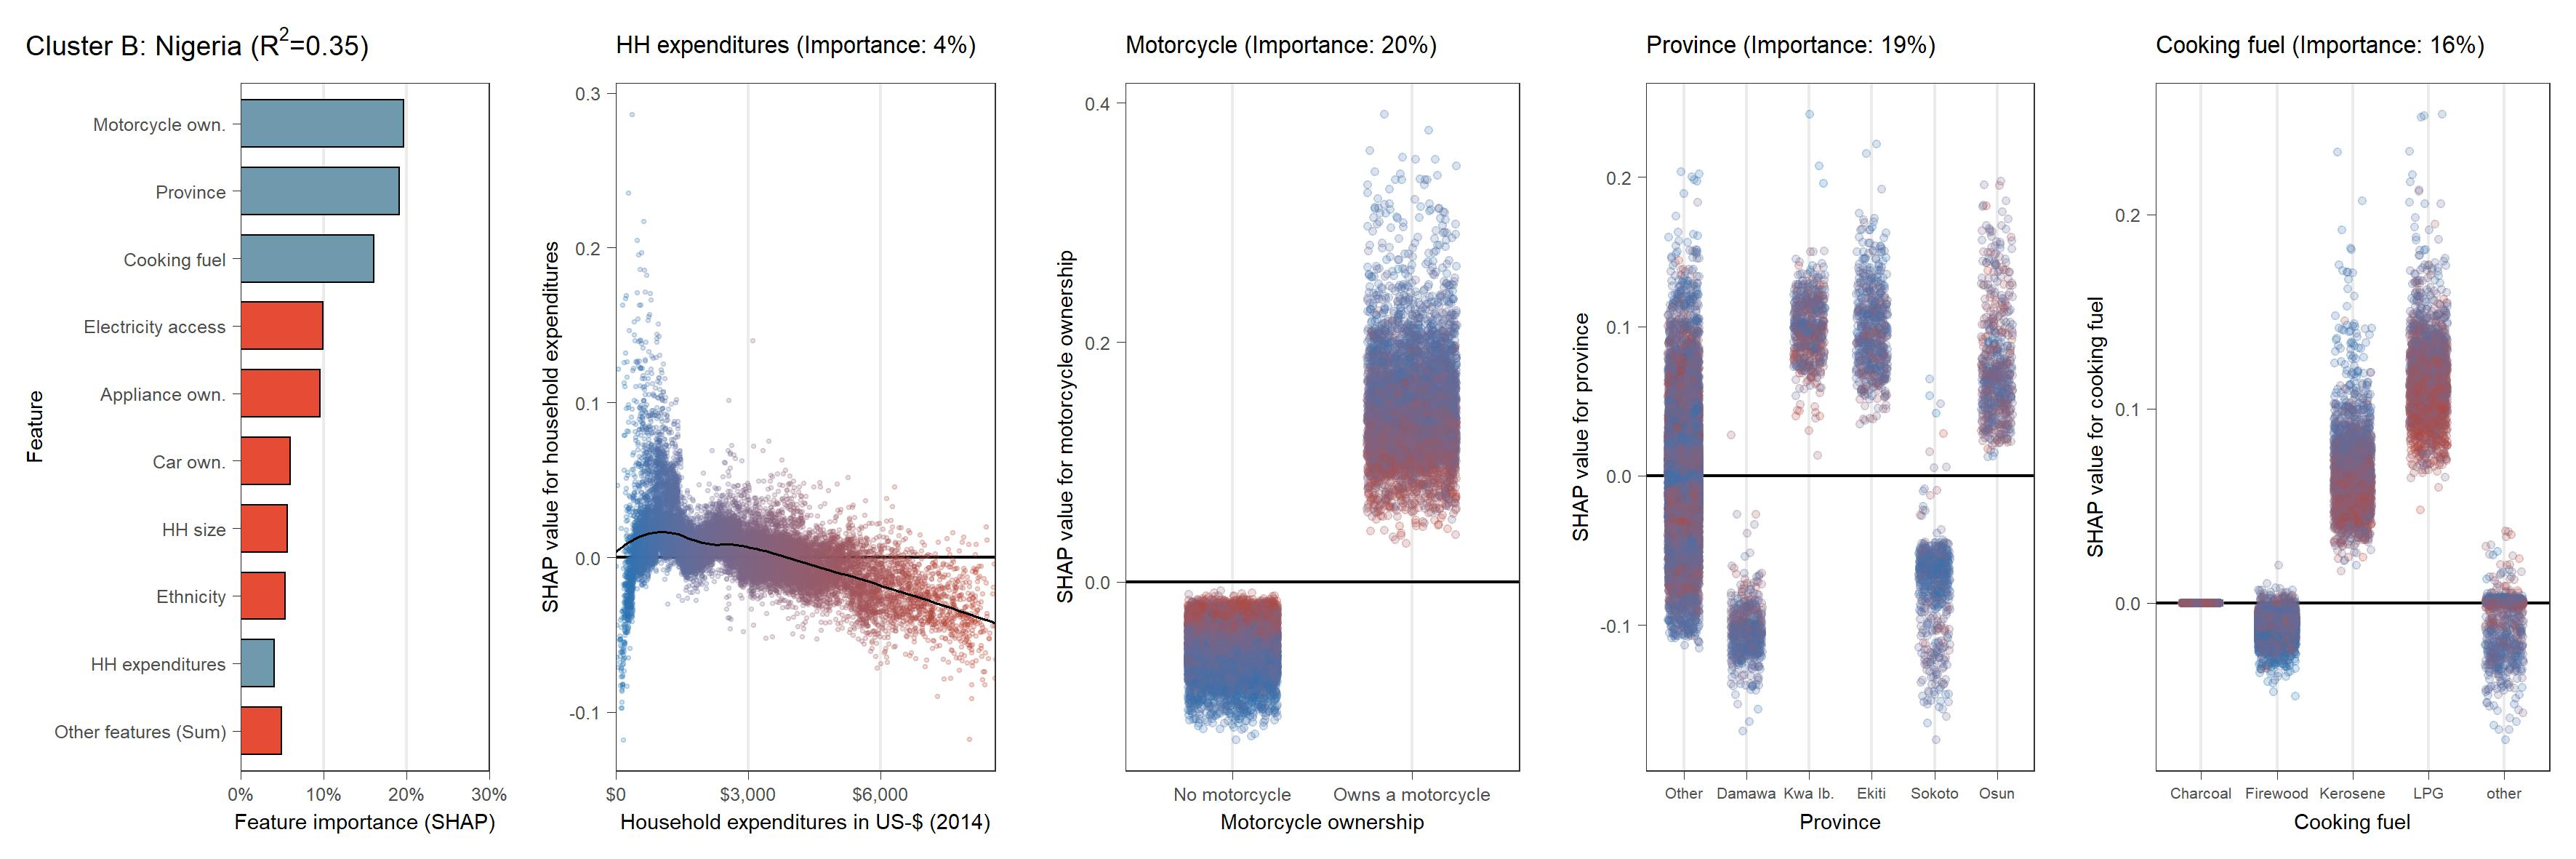
\includegraphics[width=\textwidth]{Figure_5b_NGA}
    \end{subfigure}
    \\
    \vspace{0.5cm}
    \begin{subcaption2}
     This figure shows SHAP-values for predicting carbon intensity over feature values for 87 countries in order of nine country-clusters. The bar chart displays normalized average absolute SHAP-values for all features. Features with less than 3\% of normalized SHAP-values are subsumed as "Other features (Sum)". Charts show SHAP-values over total household expenditures for all countries and for the three most important features in each country besides total household expenditures. Colors represent household expenditures with blue (red) colors indicating lower (higher) household expenditures.
     \end{subcaption2}
\end{figure}

\begin{figure}[ht!]\ContinuedFloat
    \centering
   \begin{subfigure}[b]{\textwidth}
         \centering
         \caption{Partial dependence plot (SHAP) for Nicaragua}
         \label{fig:5b_NIC}
         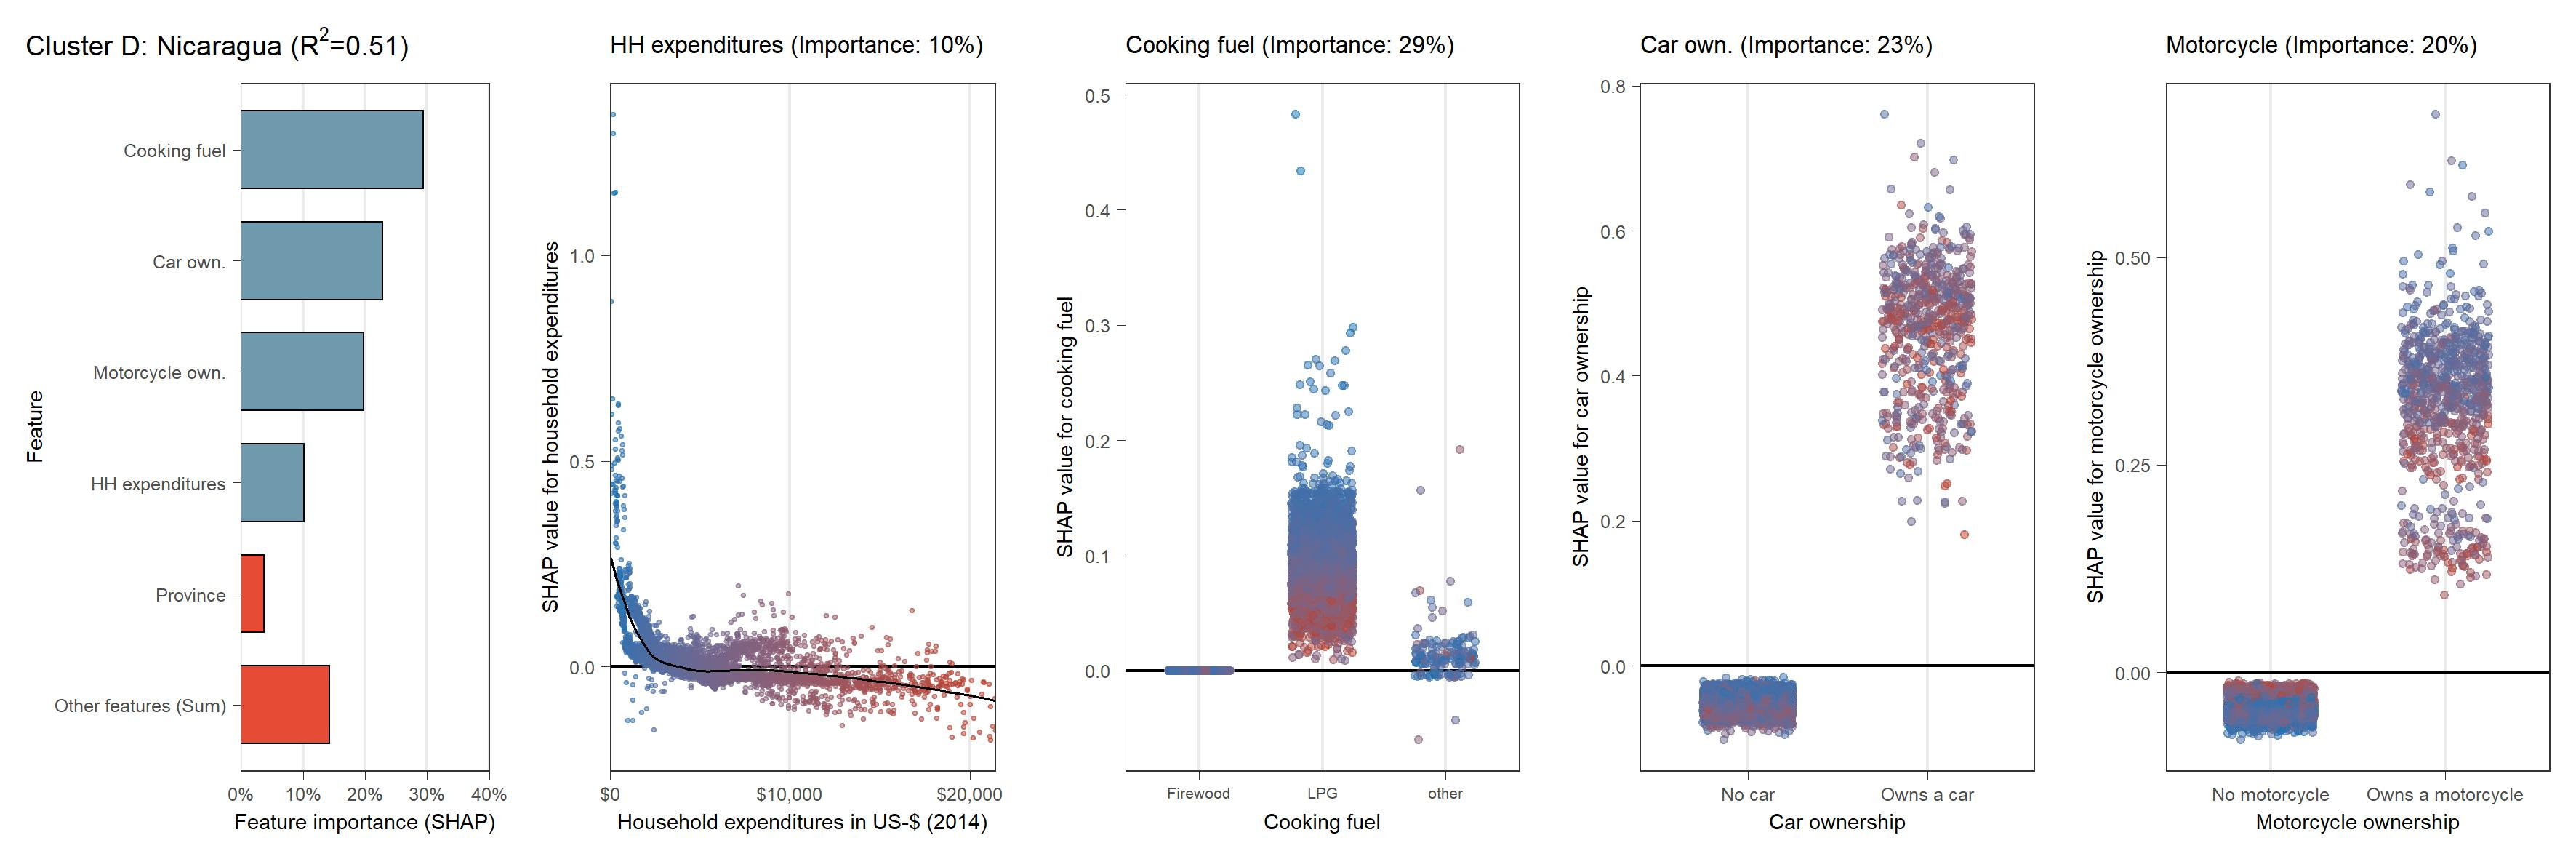
\includegraphics[width=\textwidth]{Figure_5b_NIC}         
     \end{subfigure}
    \\
    \vspace{0.5cm}
   \begin{subfigure}[b]{\textwidth}
         \centering
         \caption{Partial dependence plot (SHAP) for Malawi}
         \label{fig:5b_MWI}
         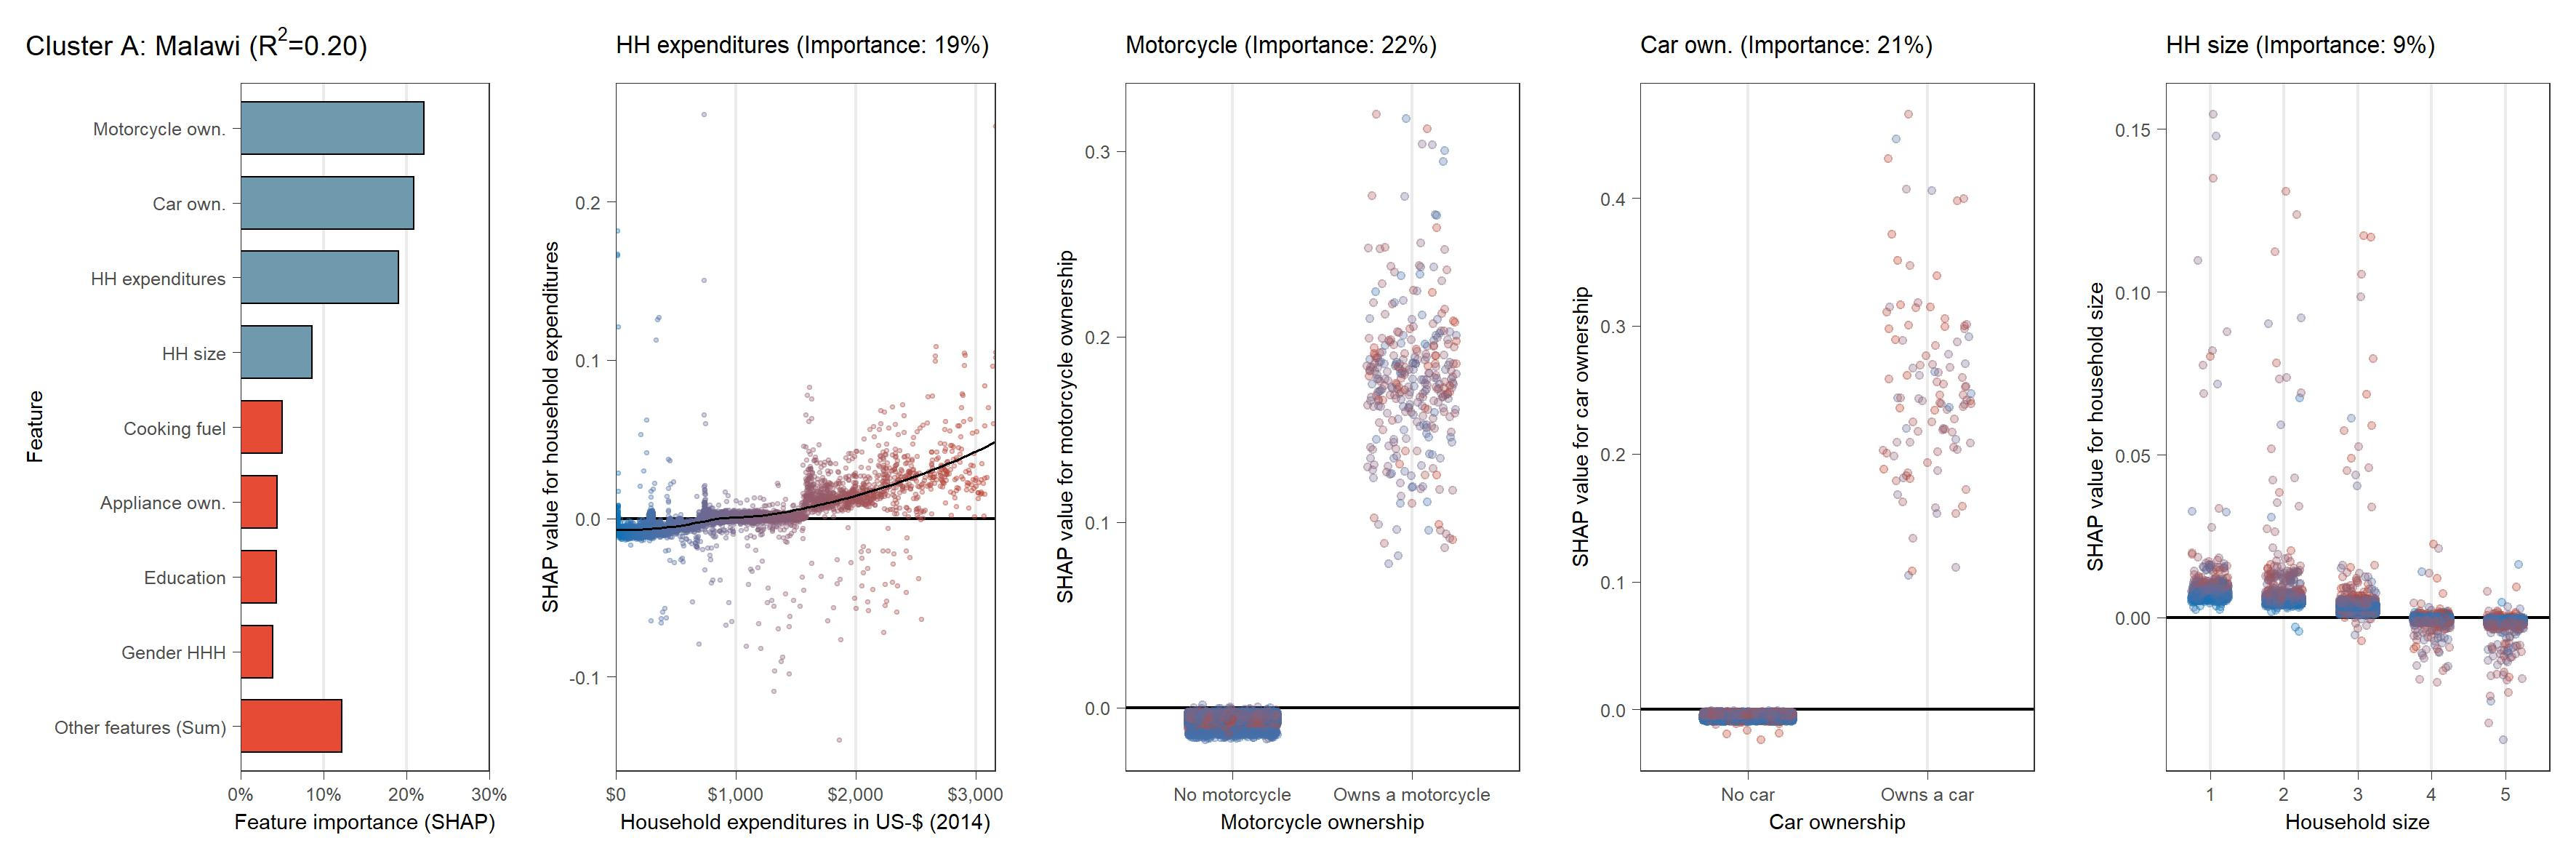
\includegraphics[width=\textwidth]{Figure_5b_MWI}         
     \end{subfigure}
    \\
    \vspace{0.5cm}
   \begin{subfigure}[b]{\textwidth}
         \centering
         \caption{Partial dependence plot (SHAP) for Guinea-Bissau}
         \label{fig:5b_GNB}
         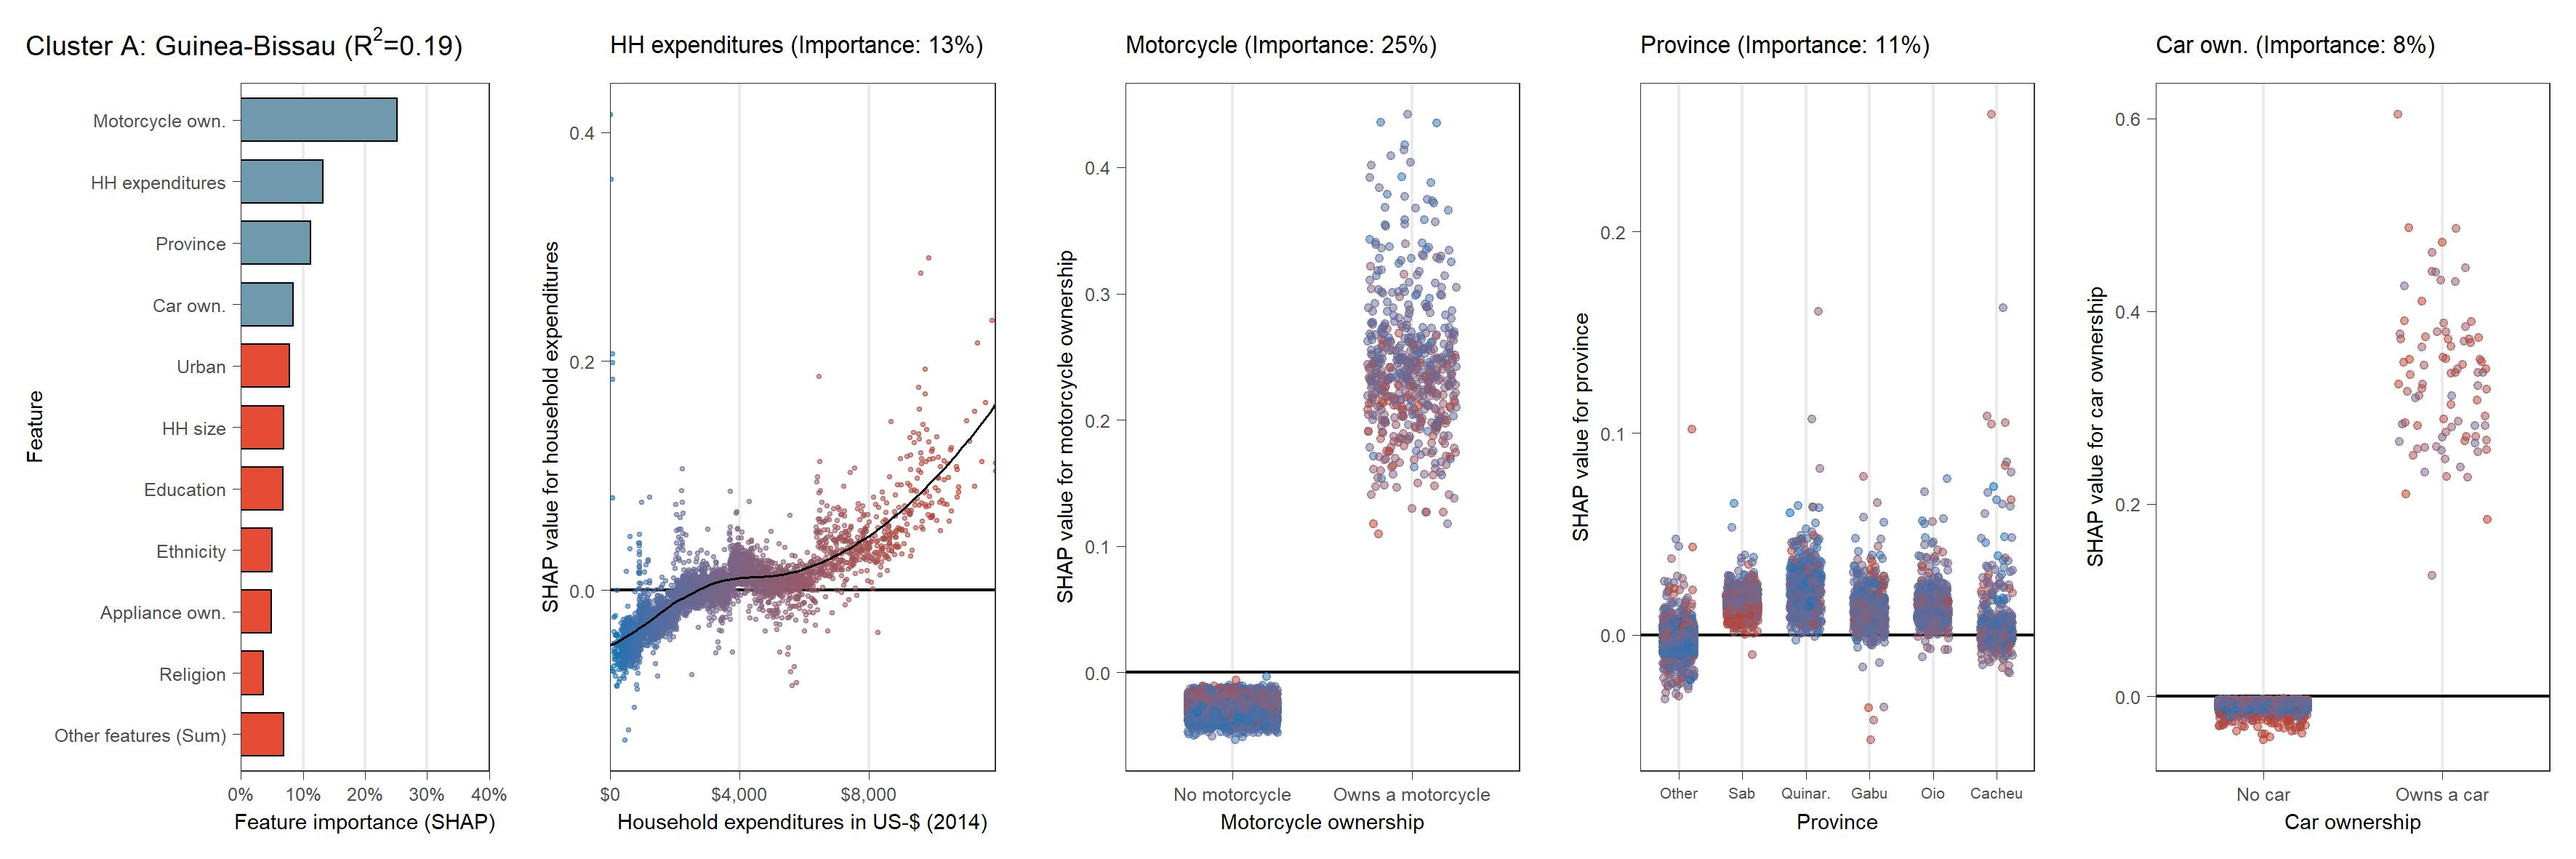
\includegraphics[width=\textwidth]{Figure_5b_GNB}
    \end{subfigure}
    \\
    \vspace{0.5cm}
    \begin{subcaption2}
     This figure shows SHAP-values for predicting carbon intensity over feature values for 87 countries in order of nine country-clusters. The bar chart displays normalized average absolute SHAP-values for all features. Features with less than 3\% of normalized SHAP-values are subsumed as "Other features (Sum)". Charts show SHAP-values over total household expenditures for all countries and for the three most important features in each country besides total household expenditures. Colors represent household expenditures with blue (red) colors indicating lower (higher) household expenditures.
     \end{subcaption2}
\end{figure}

\begin{figure}[ht!]\ContinuedFloat
    \centering
   \begin{subfigure}[b]{\textwidth}
         \centering
         \caption{Partial dependence plot (SHAP) for Suriname}
         \label{fig:5b_SUR}
         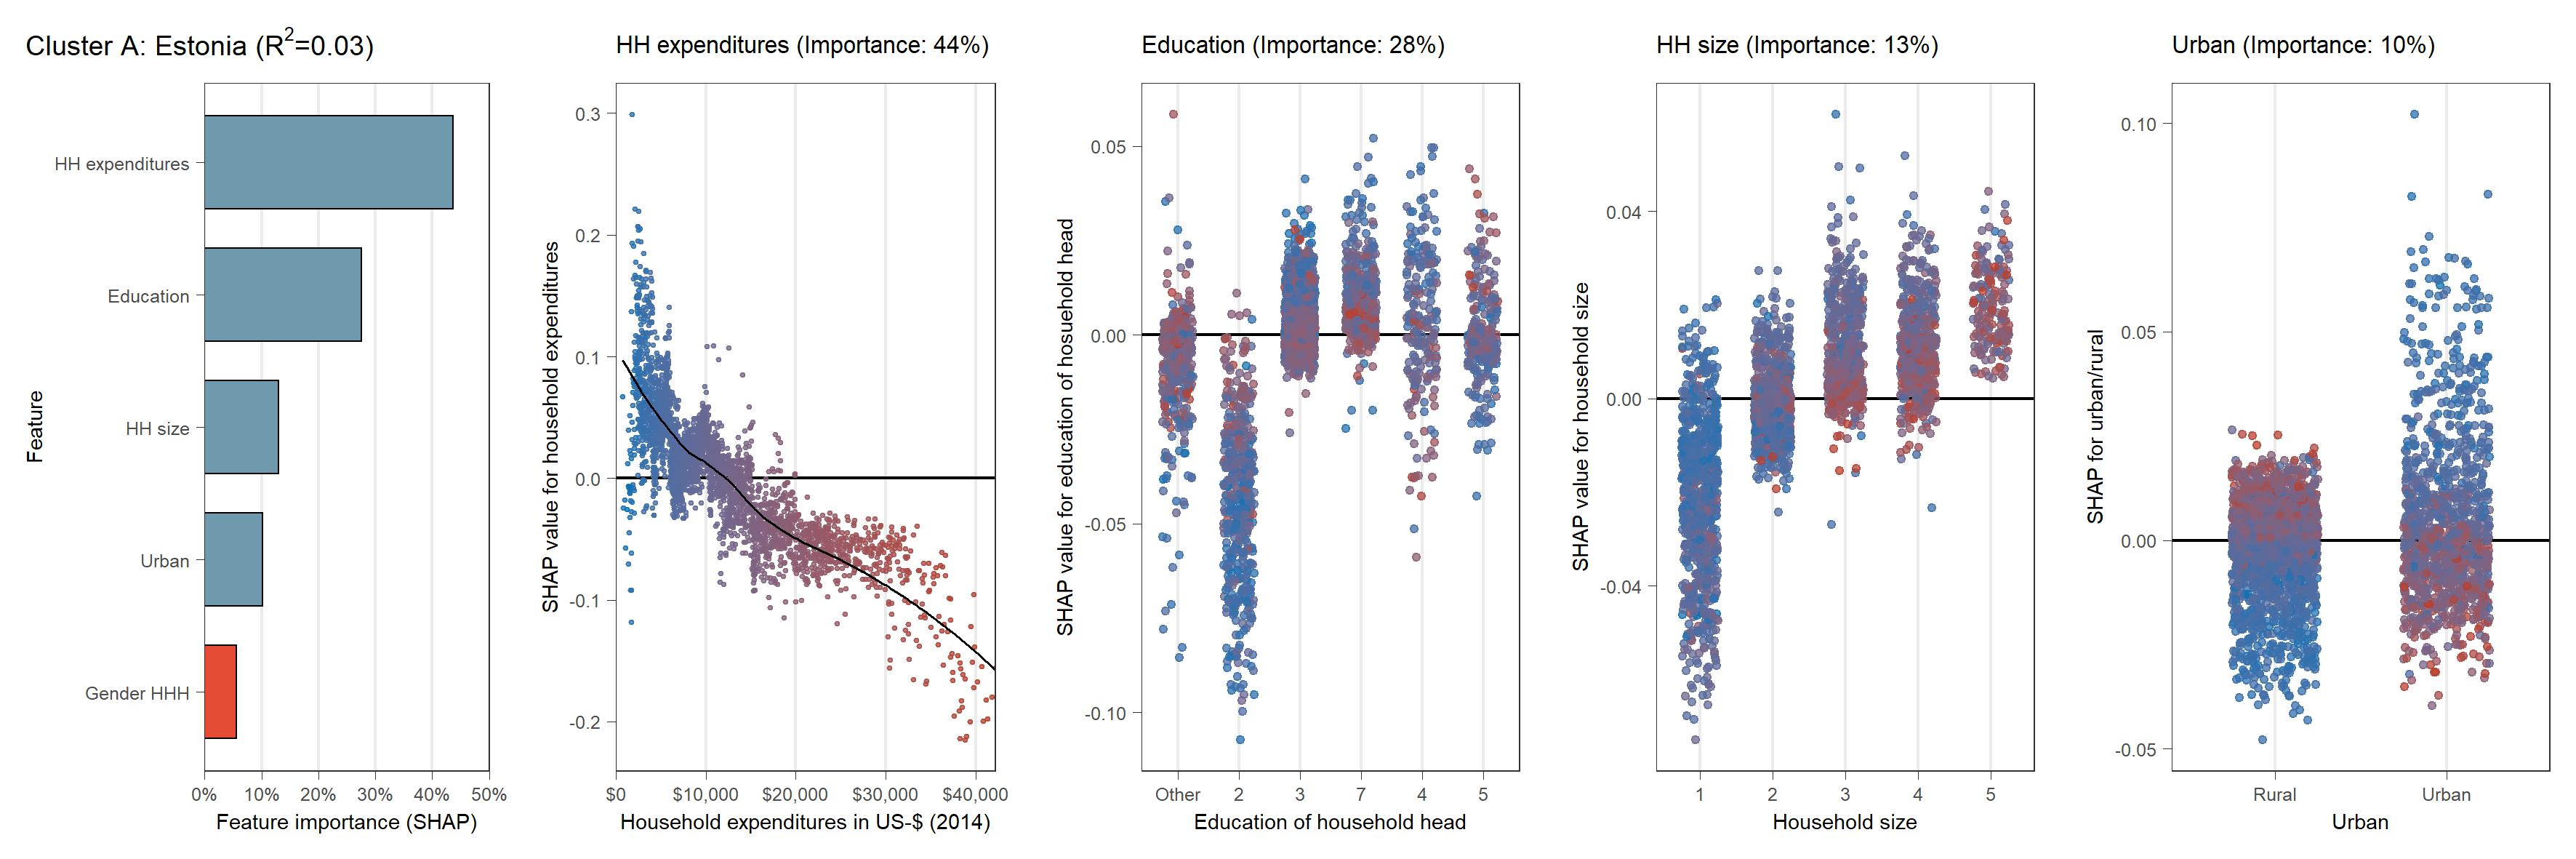
\includegraphics[width=\textwidth]{Figure_5b_EST}         
     \end{subfigure}
    \\
    \vspace{0.5cm}
   \begin{subfigure}[b]{\textwidth}
         \centering
         \caption{Partial dependence plot (SHAP) for Morocco}
         \label{fig:5b_MAR}
         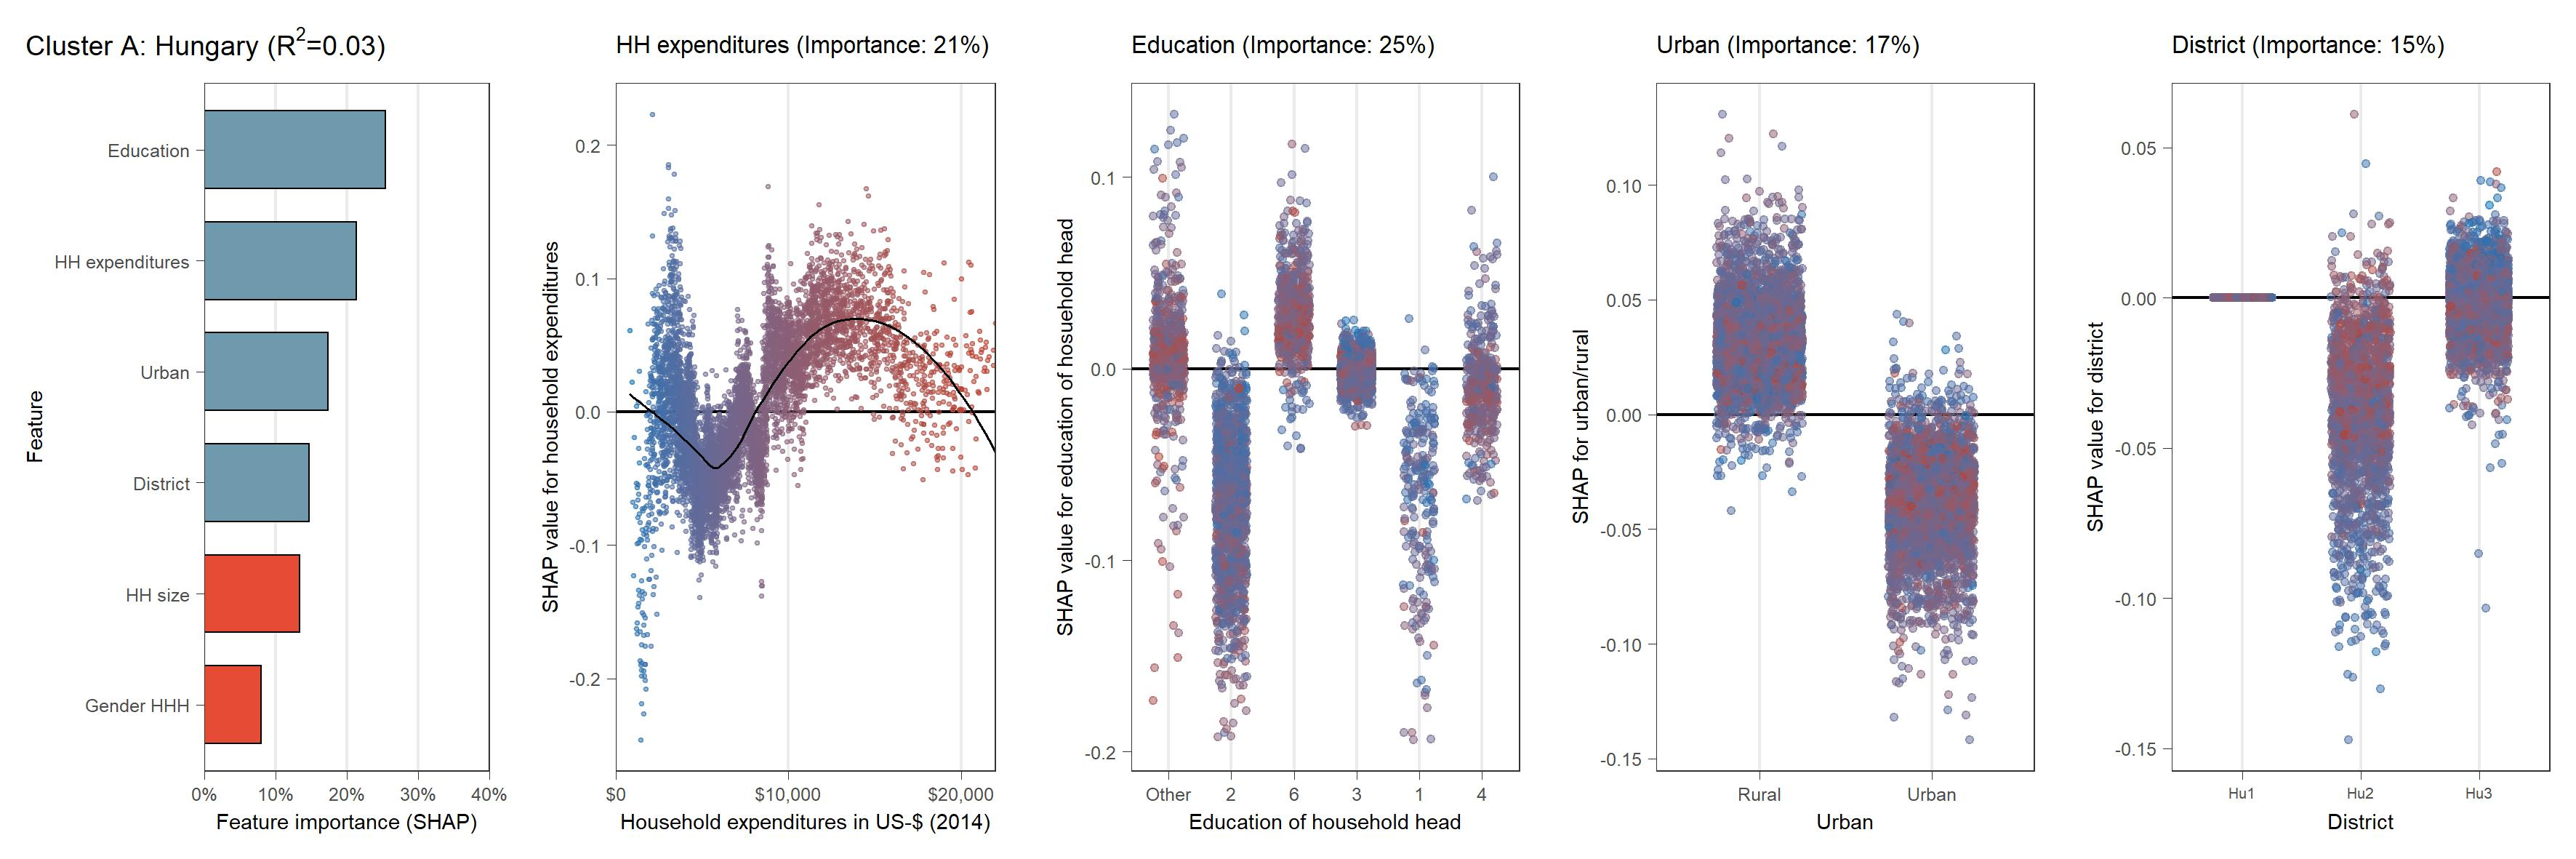
\includegraphics[width=\textwidth]{Figure_5b_HUN}         
     \end{subfigure}
    \\
    \vspace{0.5cm}
   \begin{subfigure}[b]{\textwidth}
         \centering
         \caption{Partial dependence plot (SHAP) for Greece}
         \label{fig:5b_GRC}
         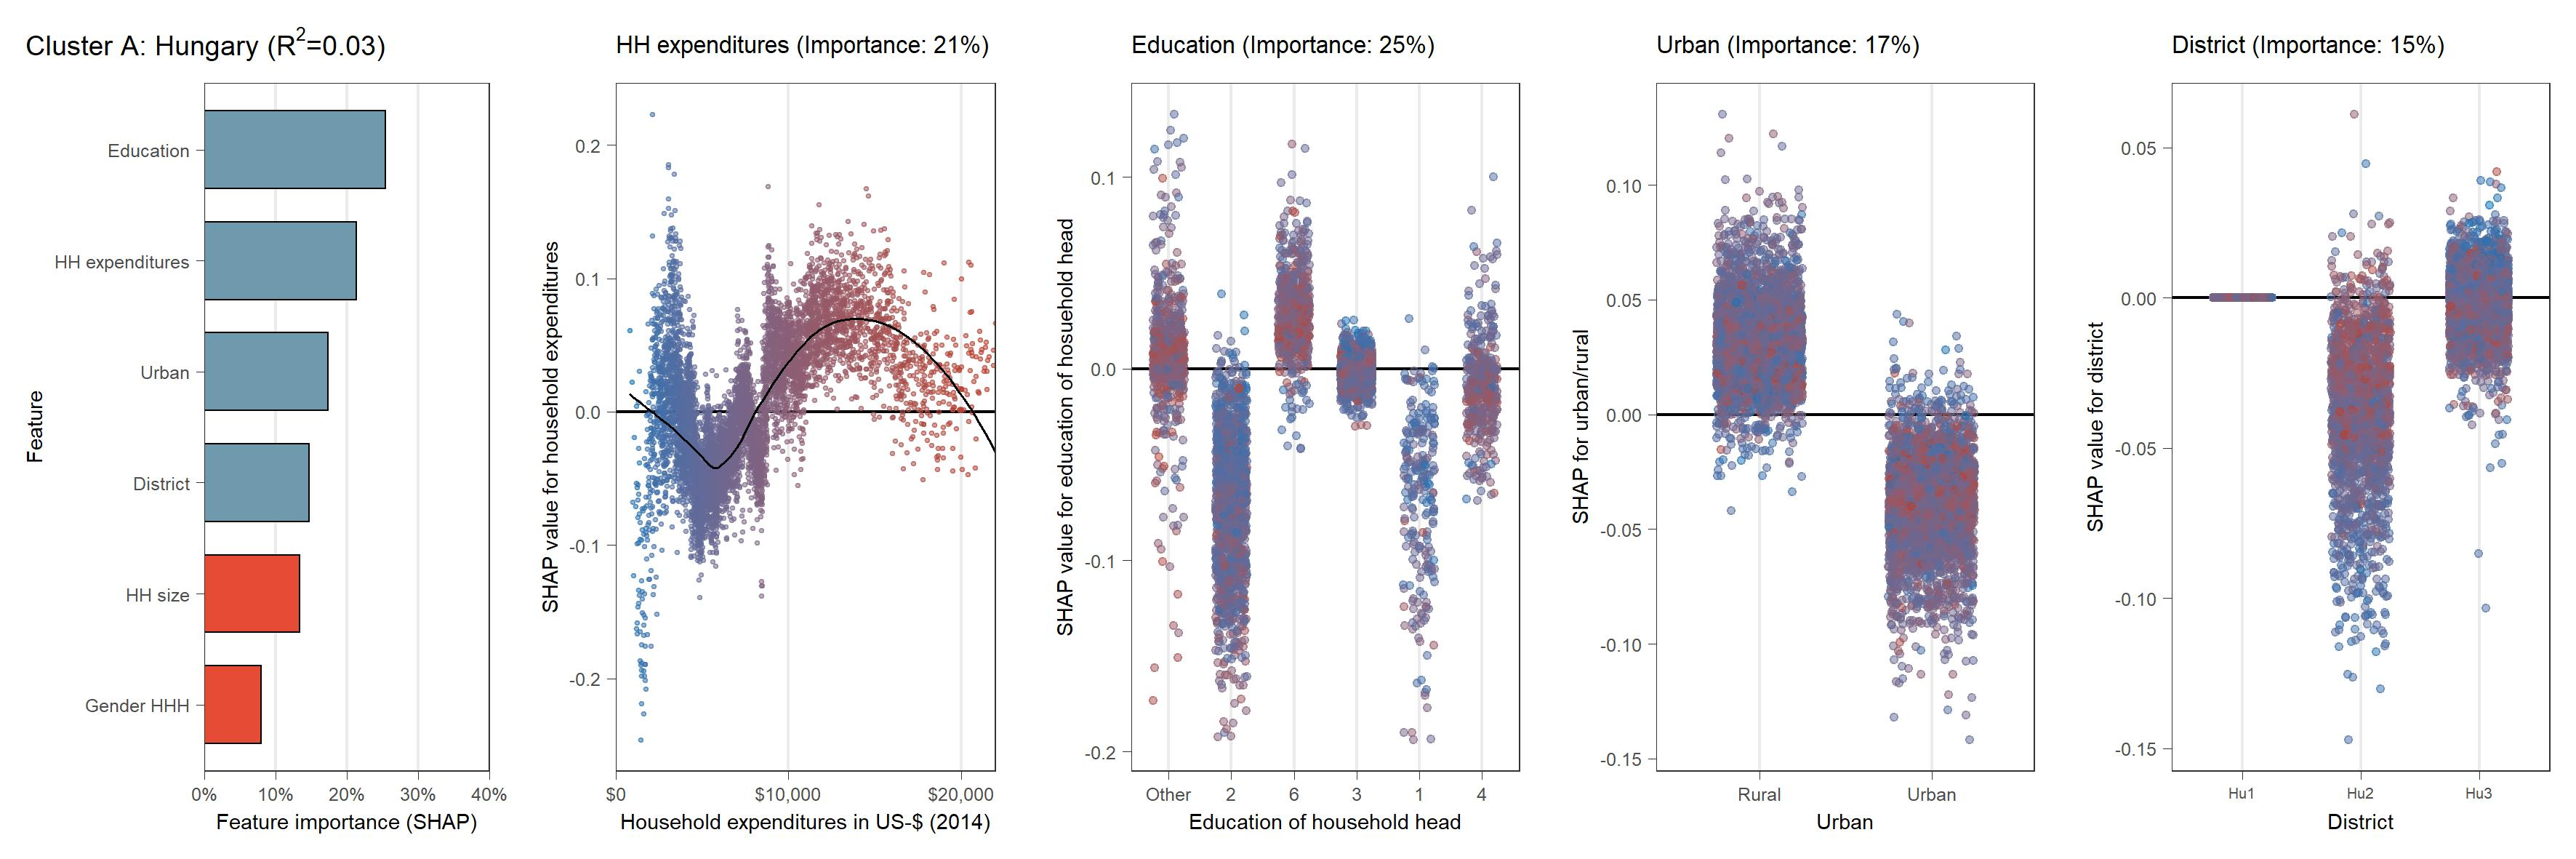
\includegraphics[width=\textwidth]{Figure_5b_HUN}
    \end{subfigure}
    \\
    \vspace{0.5cm}
    \begin{subcaption2}
     This figure shows SHAP-values for predicting carbon intensity over feature values for 87 countries in order of nine country-clusters. The bar chart displays normalized average absolute SHAP-values for all features. Features with less than 3\% of normalized SHAP-values are subsumed as "Other features (Sum)". Charts show SHAP-values over total household expenditures for all countries and for the three most important features in each country besides total household expenditures. Colors represent household expenditures with blue (red) colors indicating lower (higher) household expenditures.
     \end{subcaption2}
\end{figure}

\begin{figure}[ht!]\ContinuedFloat
    \centering
   \begin{subfigure}[b]{\textwidth}
         \centering
         \caption{Partial dependence plot (SHAP) for Suriname}
         \label{fig:5b_SUR}
         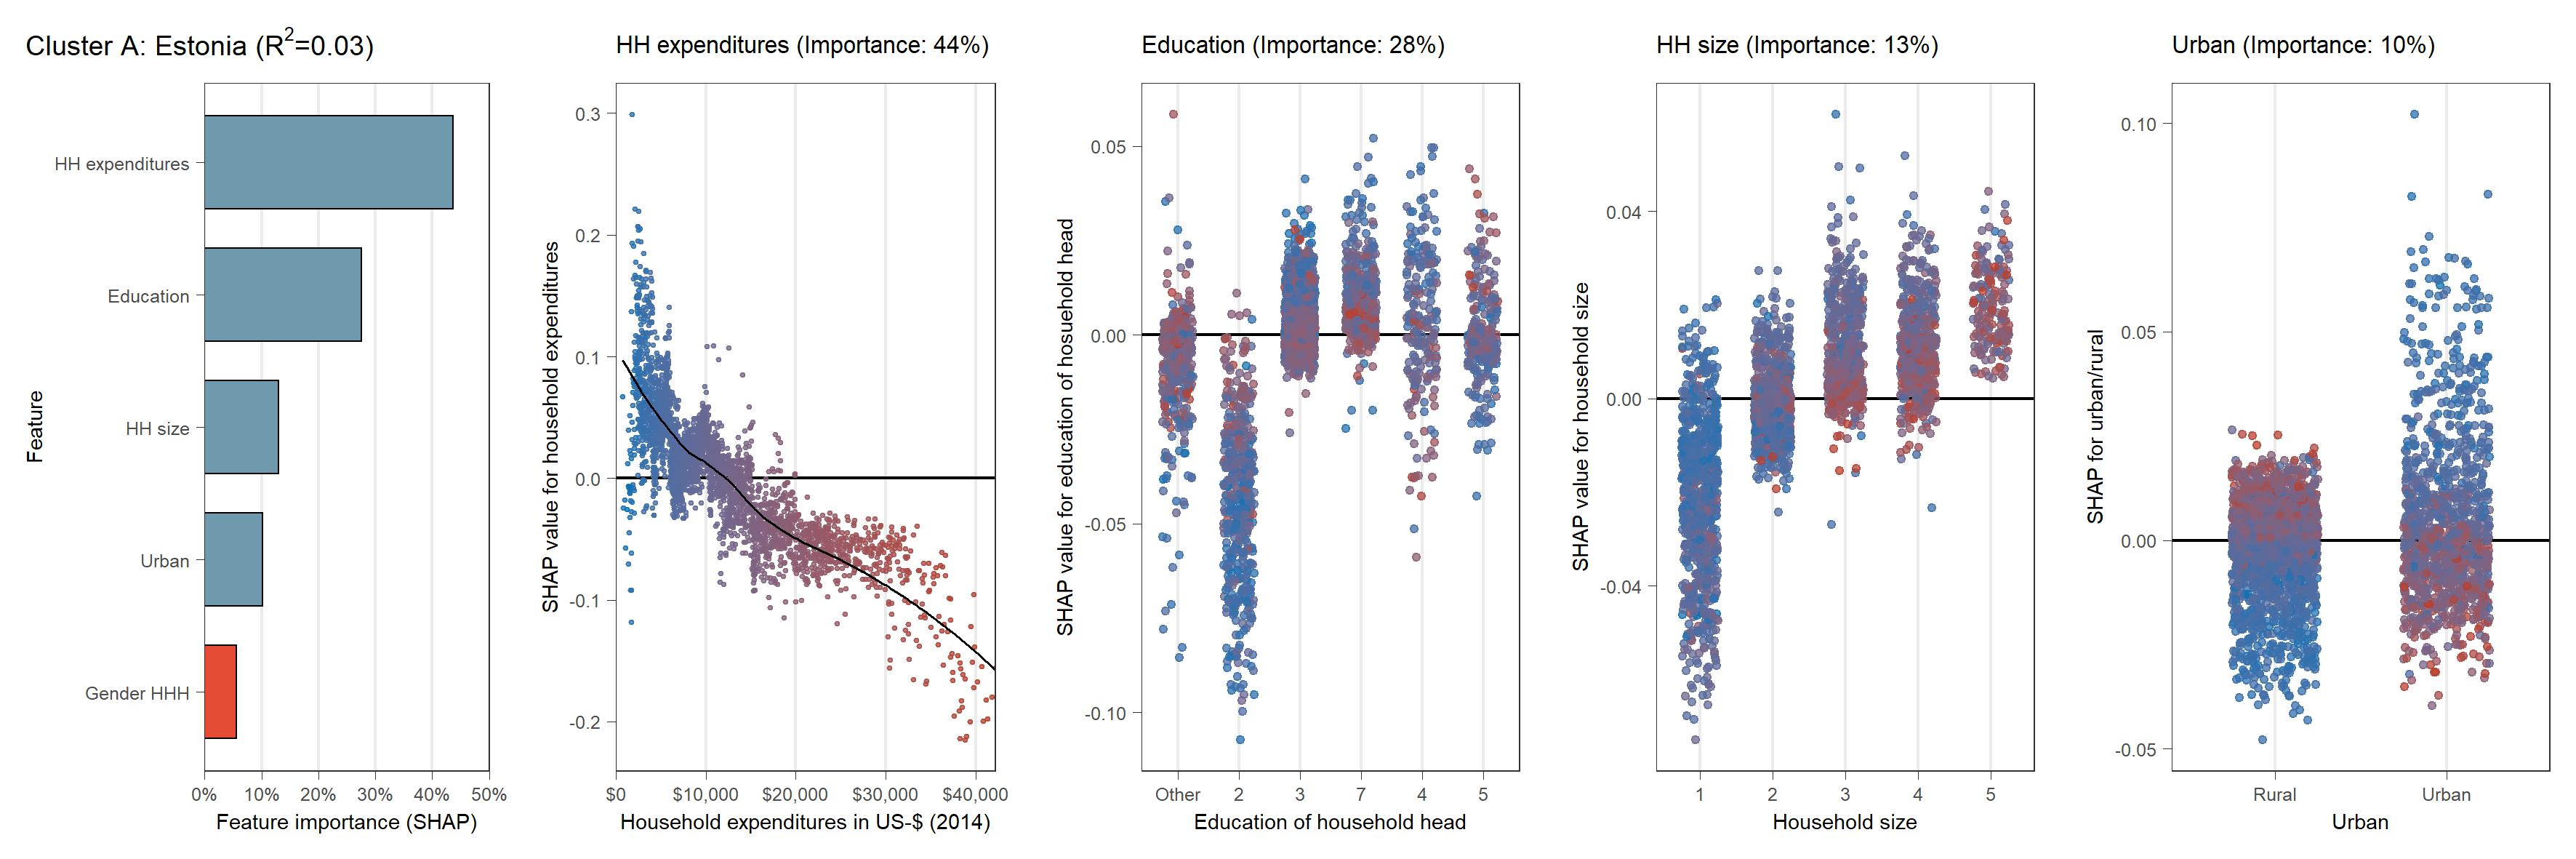
\includegraphics[width=\textwidth]{Figure_5b_EST}         
     \end{subfigure}
    \\
    \vspace{0.5cm}
   \begin{subfigure}[b]{\textwidth}
         \centering
         \caption{Partial dependence plot (SHAP) for Morocco}
         \label{fig:5b_MAR}
         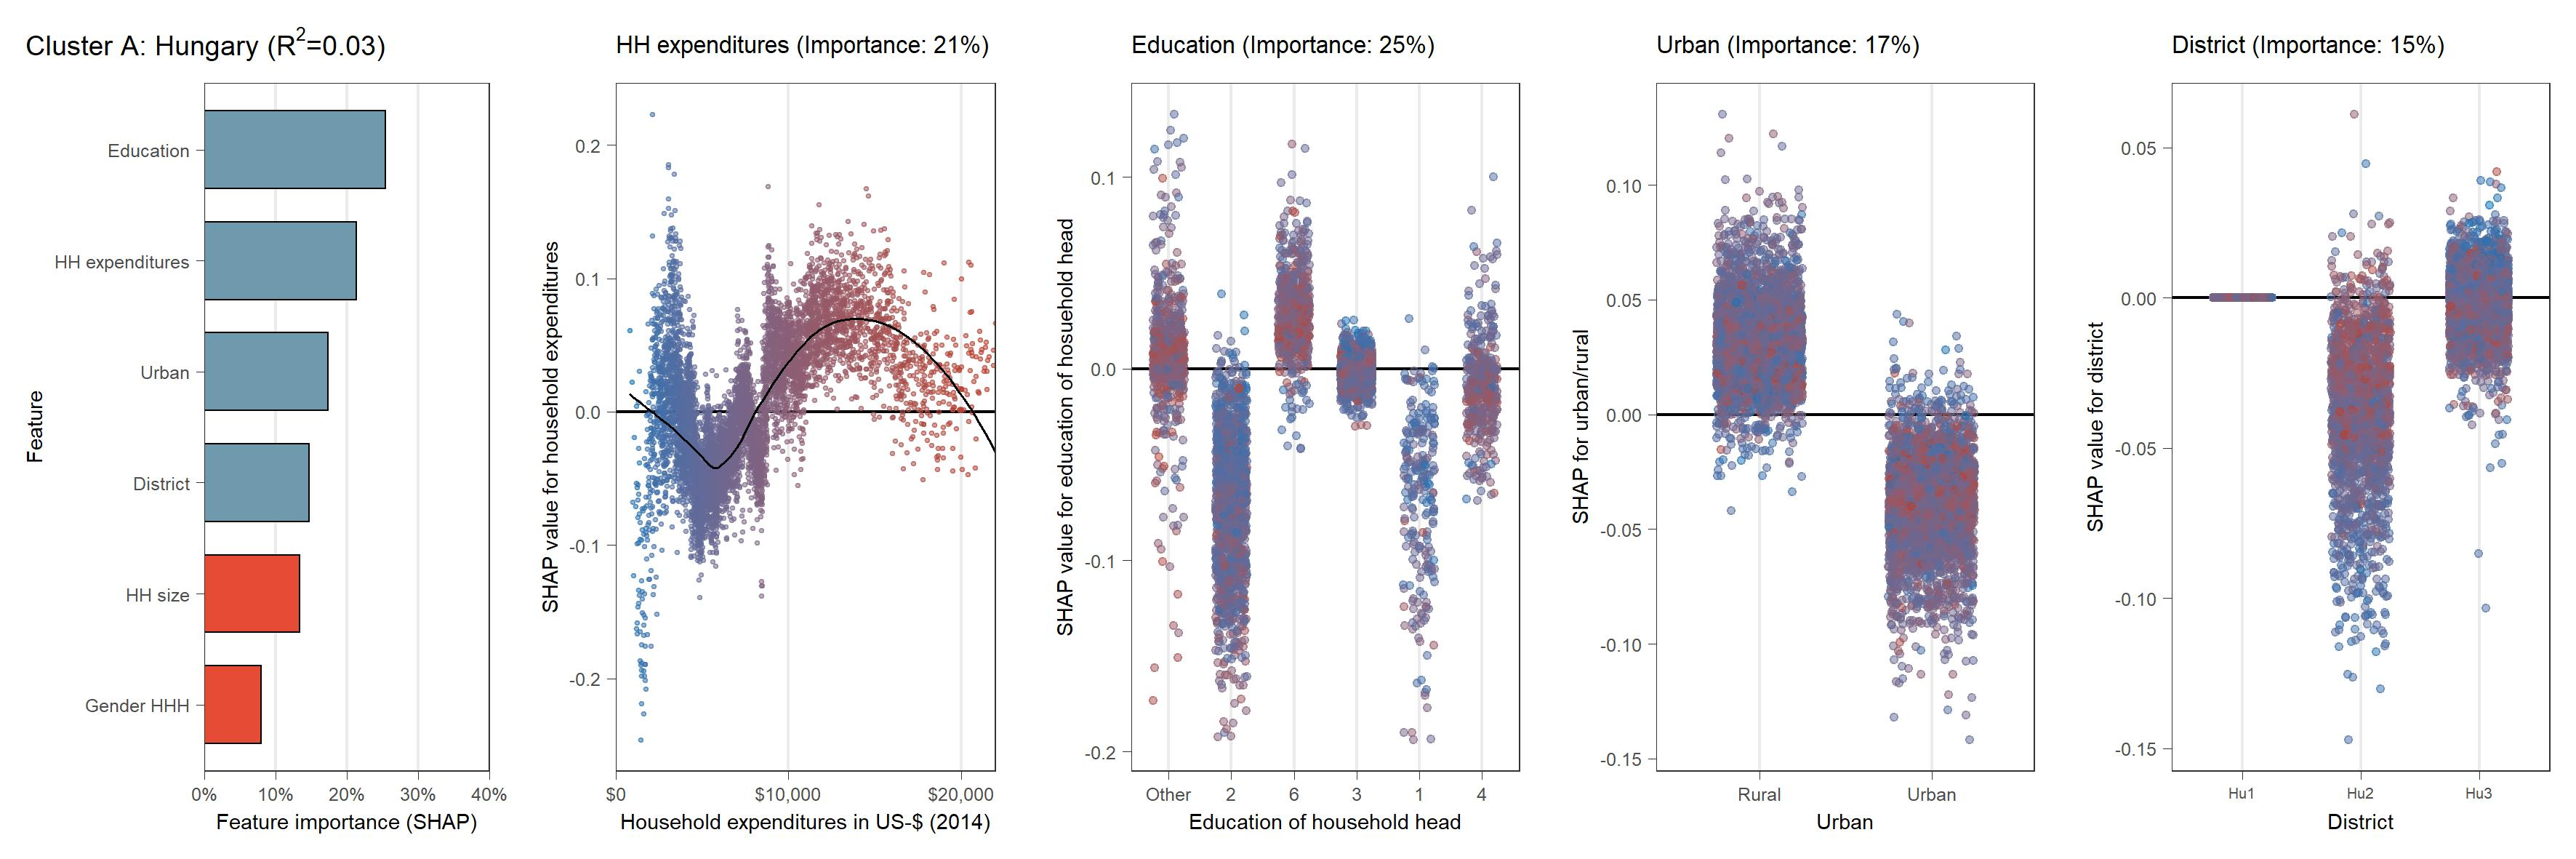
\includegraphics[width=\textwidth]{Figure_5b_HUN}         
     \end{subfigure}
    \\
    \vspace{0.5cm}
   \begin{subfigure}[b]{\textwidth}
         \centering
         \caption{Partial dependence plot (SHAP) for Greece}
         \label{fig:5b_GRC}
         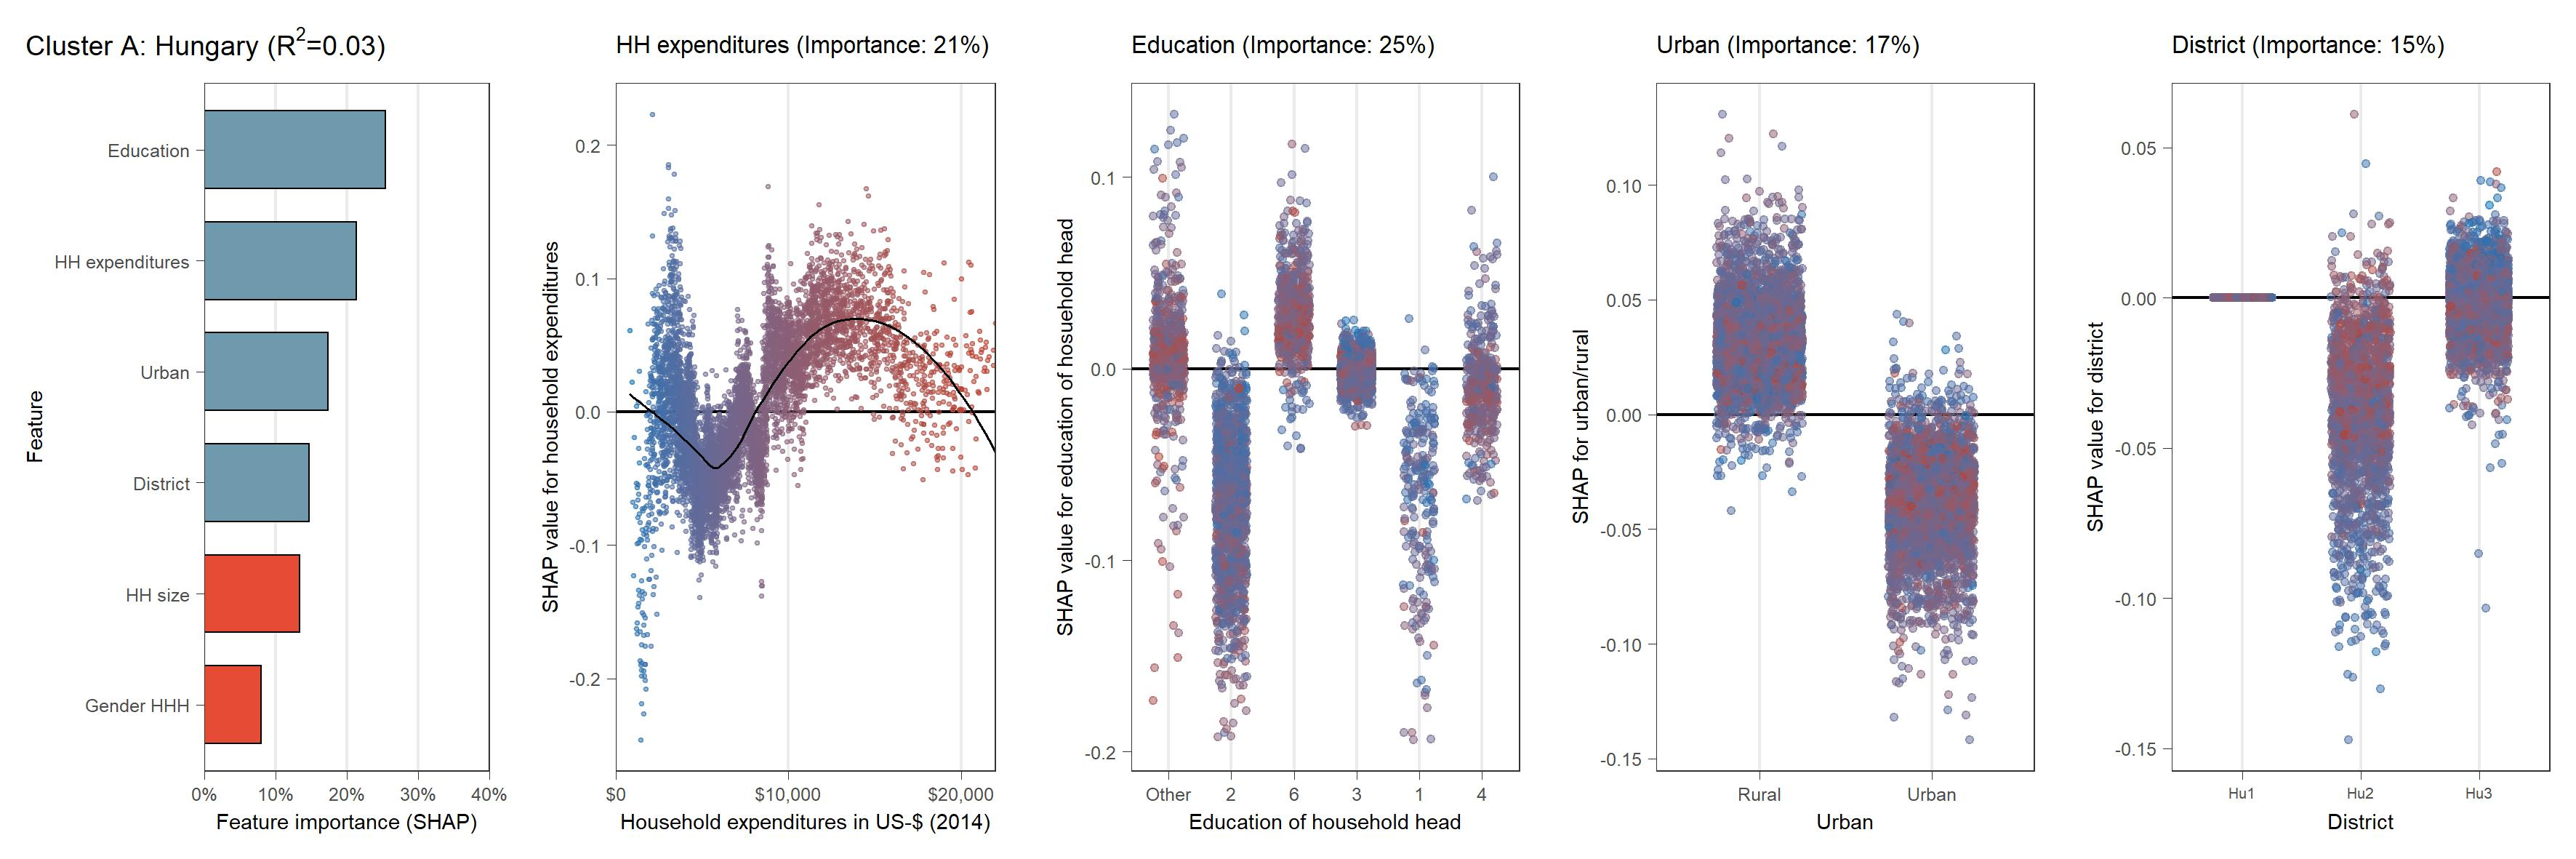
\includegraphics[width=\textwidth]{Figure_5b_HUN}
    \end{subfigure}
    \\
    \vspace{0.5cm}
    \begin{subcaption2}
     This figure shows SHAP-values for predicting carbon intensity over feature values for 87 countries in order of nine country-clusters. The bar chart displays normalized average absolute SHAP-values for all features. Features with less than 3\% of normalized SHAP-values are subsumed as "Other features (Sum)". Charts show SHAP-values over total household expenditures for all countries and for the three most important features in each country besides total household expenditures. Colors represent household expenditures with blue (red) colors indicating lower (higher) household expenditures.
     \end{subcaption2}
\end{figure}

\begin{figure}[ht!]\ContinuedFloat
    \centering
   \begin{subfigure}[b]{\textwidth}
         \centering
         \caption{Partial dependence plot (SHAP) for Suriname}
         \label{fig:5b_SUR}
         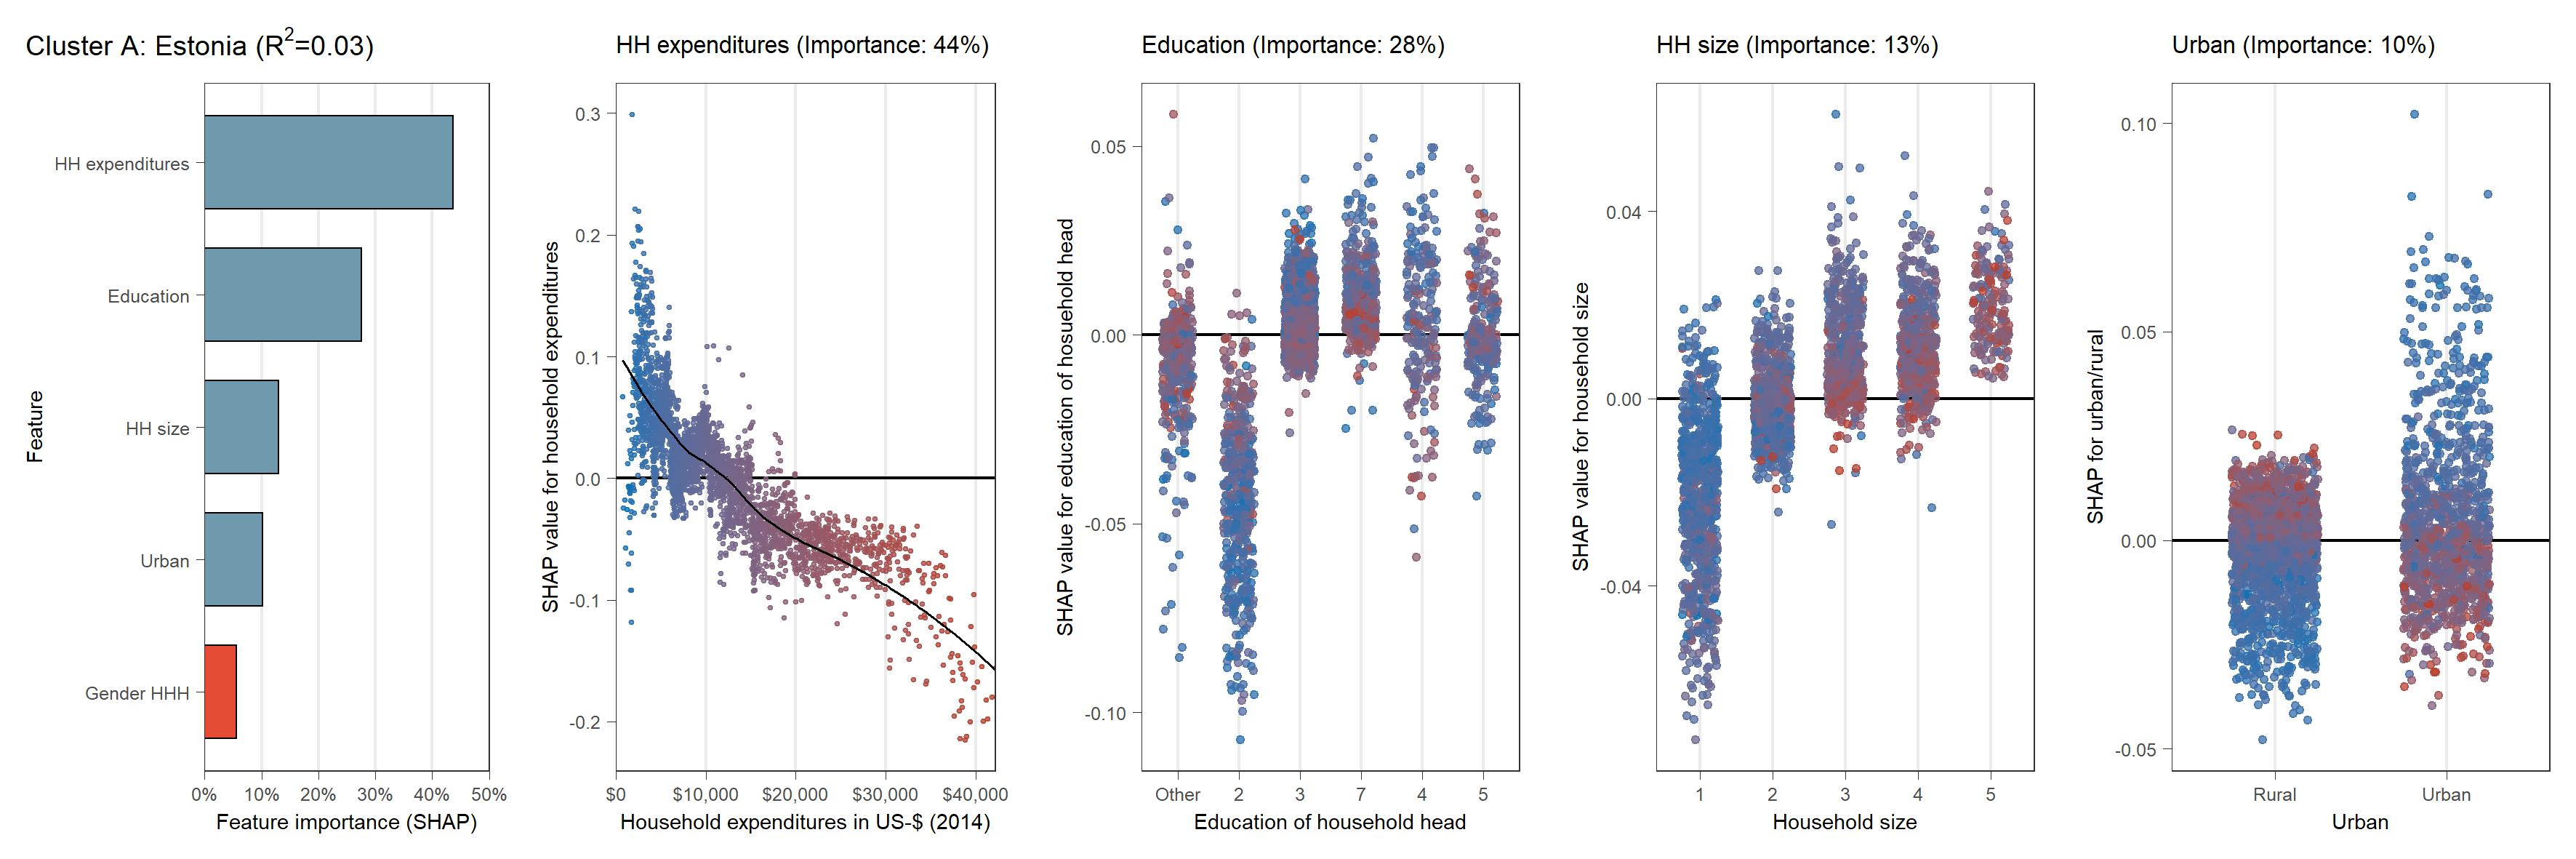
\includegraphics[width=\textwidth]{Figure_5b_EST}         
     \end{subfigure}
    \\
    \vspace{0.5cm}
   \begin{subfigure}[b]{\textwidth}
         \centering
         \caption{Partial dependence plot (SHAP) for Morocco}
         \label{fig:5b_MAR}
         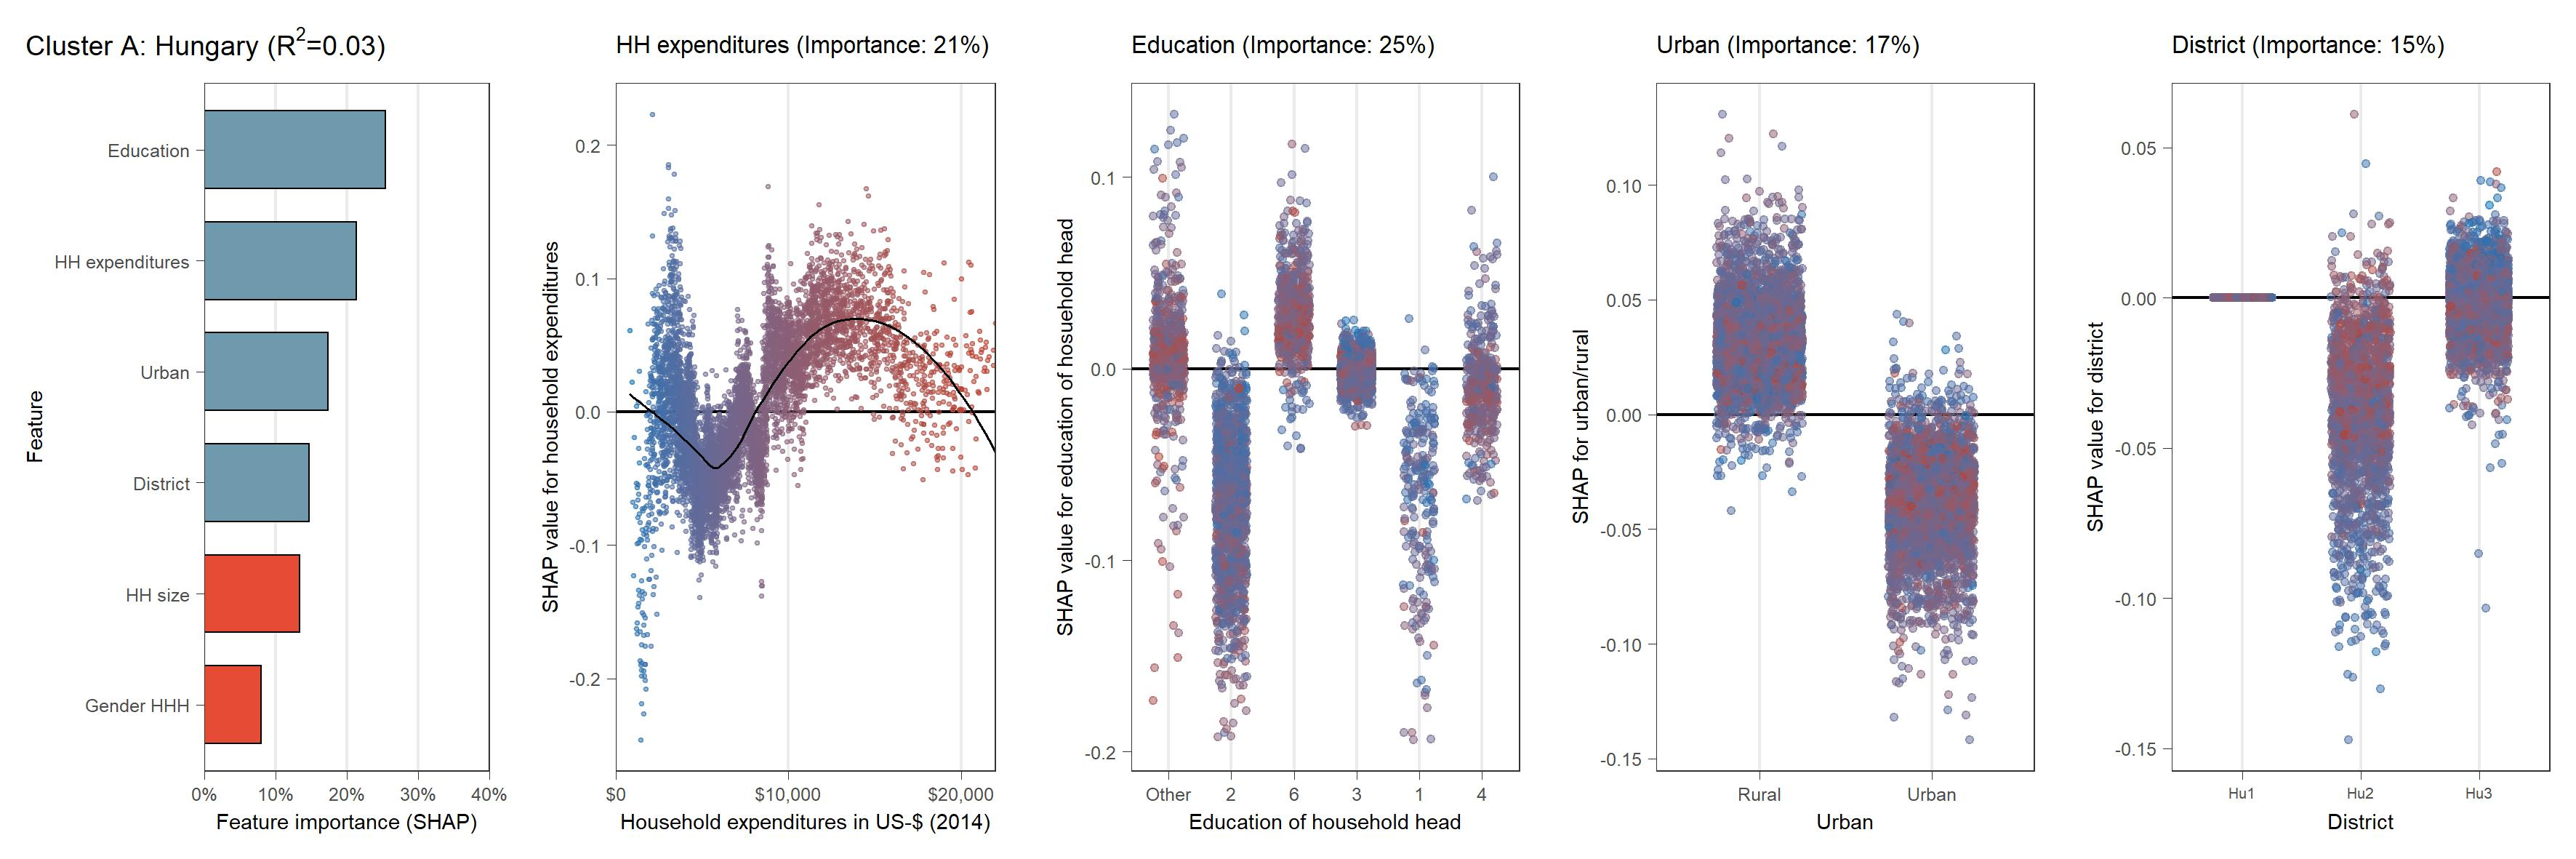
\includegraphics[width=\textwidth]{Figure_5b_HUN}         
     \end{subfigure}
    \\
    \vspace{0.5cm}
   \begin{subfigure}[b]{\textwidth}
         \centering
         \caption{Partial dependence plot (SHAP) for Greece}
         \label{fig:5b_GRC}
         \includegraphics[width=\textwidth]{Figure_5b_HUN}
    \end{subfigure}
    \\
    \vspace{0.5cm}
    \begin{subcaption2}
     This figure shows SHAP-values for predicting carbon intensity over feature values for 87 countries in order of nine country-clusters. The bar chart displays normalized average absolute SHAP-values for all features. Features with less than 3\% of normalized SHAP-values are subsumed as "Other features (Sum)". Charts show SHAP-values over total household expenditures for all countries and for the three most important features in each country besides total household expenditures. Colors represent household expenditures with blue (red) colors indicating lower (higher) household expenditures.
     \end{subcaption2}
\end{figure}

\begin{figure}[ht!]\ContinuedFloat
    \centering
   \begin{subfigure}[b]{\textwidth}
         \centering
         \caption{Partial dependence plot (SHAP) for Suriname}
         \label{fig:5b_SUR}
         \includegraphics[width=\textwidth]{Figure_5b_EST}         
     \end{subfigure}
    \\
    \vspace{0.5cm}
   \begin{subfigure}[b]{\textwidth}
         \centering
         \caption{Partial dependence plot (SHAP) for Morocco}
         \label{fig:5b_MAR}
         \includegraphics[width=\textwidth]{Figure_5b_HUN}         
     \end{subfigure}
    \\
    \vspace{0.5cm}
   \begin{subfigure}[b]{\textwidth}
         \centering
         \caption{Partial dependence plot (SHAP) for Greece}
         \label{fig:5b_GRC}
         \includegraphics[width=\textwidth]{Figure_5b_HUN}
    \end{subfigure}
    \\
    \vspace{0.5cm}
    \begin{subcaption2}
     This figure shows SHAP-values for predicting carbon intensity over feature values for 87 countries in order of nine country-clusters. The bar chart displays normalized average absolute SHAP-values for all features. Features with less than 3\% of normalized SHAP-values are subsumed as "Other features (Sum)". Charts show SHAP-values over total household expenditures for all countries and for the three most important features in each country besides total household expenditures. Colors represent household expenditures with blue (red) colors indicating lower (higher) household expenditures.
     \end{subcaption2}
\end{figure}

\begin{figure}[ht!]\ContinuedFloat
    \centering
   \begin{subfigure}[b]{\textwidth}
         \centering
         \caption{Partial dependence plot (SHAP) for Suriname}
         \label{fig:5b_SUR}
         \includegraphics[width=\textwidth]{Figure_5b_EST}         
     \end{subfigure}
    \\
    \vspace{0.5cm}
   \begin{subfigure}[b]{\textwidth}
         \centering
         \caption{Partial dependence plot (SHAP) for Morocco}
         \label{fig:5b_MAR}
         \includegraphics[width=\textwidth]{Figure_5b_HUN}         
     \end{subfigure}
    \\
    \vspace{0.5cm}
   \begin{subfigure}[b]{\textwidth}
         \centering
         \caption{Partial dependence plot (SHAP) for Greece}
         \label{fig:5b_GRC}
         \includegraphics[width=\textwidth]{Figure_5b_HUN}
    \end{subfigure}
    \\
    \vspace{0.5cm}
    \begin{subcaption2}
     This figure shows SHAP-values for predicting carbon intensity over feature values for 87 countries in order of nine country-clusters. The bar chart displays normalized average absolute SHAP-values for all features. Features with less than 3\% of normalized SHAP-values are subsumed as "Other features (Sum)". Charts show SHAP-values over total household expenditures for all countries and for the three most important features in each country besides total household expenditures. Colors represent household expenditures with blue (red) colors indicating lower (higher) household expenditures.
     \end{subcaption2}
\end{figure}

\begin{figure}[ht!]\ContinuedFloat
    \centering
   \begin{subfigure}[b]{\textwidth}
         \centering
         \caption{Partial dependence plot (SHAP) for Suriname}
         \label{fig:5b_SUR}
         \includegraphics[width=\textwidth]{Figure_5b_EST}         
     \end{subfigure}
    \\
    \vspace{0.5cm}
   \begin{subfigure}[b]{\textwidth}
         \centering
         \caption{Partial dependence plot (SHAP) for Morocco}
         \label{fig:5b_MAR}
         \includegraphics[width=\textwidth]{Figure_5b_HUN}         
     \end{subfigure}
    \\
    \vspace{0.5cm}
   \begin{subfigure}[b]{\textwidth}
         \centering
         \caption{Partial dependence plot (SHAP) for Greece}
         \label{fig:5b_GRC}
         \includegraphics[width=\textwidth]{Figure_5b_HUN}
    \end{subfigure}
    \\
    \vspace{0.5cm}
    \begin{subcaption2}
     This figure shows SHAP-values for predicting carbon intensity over feature values for 87 countries in order of nine country-clusters. The bar chart displays normalized average absolute SHAP-values for all features. Features with less than 3\% of normalized SHAP-values are subsumed as "Other features (Sum)". Charts show SHAP-values over total household expenditures for all countries and for the three most important features in each country besides total household expenditures. Colors represent household expenditures with blue (red) colors indicating lower (higher) household expenditures.
     \end{subcaption2}
\end{figure}

\begin{figure}[ht!]\ContinuedFloat
    \centering
   \begin{subfigure}[b]{\textwidth}
         \centering
         \caption{Partial dependence plot (SHAP) for Suriname}
         \label{fig:5b_SUR}
         \includegraphics[width=\textwidth]{Figure_5b_EST}         
     \end{subfigure}
    \\
    \vspace{0.5cm}
   \begin{subfigure}[b]{\textwidth}
         \centering
         \caption{Partial dependence plot (SHAP) for Morocco}
         \label{fig:5b_MAR}
         \includegraphics[width=\textwidth]{Figure_5b_HUN}         
     \end{subfigure}
    \\
    \vspace{0.5cm}
   \begin{subfigure}[b]{\textwidth}
         \centering
         \caption{Partial dependence plot (SHAP) for Greece}
         \label{fig:5b_GRC}
         \includegraphics[width=\textwidth]{Figure_5b_HUN}
    \end{subfigure}
    \\
    \vspace{0.5cm}
    \begin{subcaption2}
     This figure shows SHAP-values for predicting carbon intensity over feature values for 87 countries in order of nine country-clusters. The bar chart displays normalized average absolute SHAP-values for all features. Features with less than 3\% of normalized SHAP-values are subsumed as "Other features (Sum)". Charts show SHAP-values over total household expenditures for all countries and for the three most important features in each country besides total household expenditures. Colors represent household expenditures with blue (red) colors indicating lower (higher) household expenditures.
     \end{subcaption2}
\end{figure}

\begin{figure}[ht!]\ContinuedFloat
    \centering
   \begin{subfigure}[b]{\textwidth}
         \centering
         \caption{Partial dependence plot (SHAP) for Suriname}
         \label{fig:5b_SUR}
         \includegraphics[width=\textwidth]{Figure_5b_EST}         
     \end{subfigure}
    \\
    \vspace{0.5cm}
   \begin{subfigure}[b]{\textwidth}
         \centering
         \caption{Partial dependence plot (SHAP) for Morocco}
         \label{fig:5b_MAR}
         \includegraphics[width=\textwidth]{Figure_5b_HUN}         
     \end{subfigure}
    \\
    \vspace{0.5cm}
   \begin{subfigure}[b]{\textwidth}
         \centering
         \caption{Partial dependence plot (SHAP) for Greece}
         \label{fig:5b_GRC}
         \includegraphics[width=\textwidth]{Figure_5b_HUN}
    \end{subfigure}
    \\
    \vspace{0.5cm}
    \begin{subcaption2}
     This figure shows SHAP-values for predicting carbon intensity over feature values for 87 countries in order of nine country-clusters. The bar chart displays normalized average absolute SHAP-values for all features. Features with less than 3\% of normalized SHAP-values are subsumed as "Other features (Sum)". Charts show SHAP-values over total household expenditures for all countries and for the three most important features in each country besides total household expenditures. Colors represent household expenditures with blue (red) colors indicating lower (higher) household expenditures.
     \end{subcaption2}
\end{figure}

\begin{figure}[ht!]\ContinuedFloat
    \centering
   \begin{subfigure}[b]{\textwidth}
         \centering
         \caption{Partial dependence plot (SHAP) for Suriname}
         \label{fig:5b_SUR}
         \includegraphics[width=\textwidth]{Figure_5b_EST}         
     \end{subfigure}
    \\
    \vspace{0.5cm}
   \begin{subfigure}[b]{\textwidth}
         \centering
         \caption{Partial dependence plot (SHAP) for Morocco}
         \label{fig:5b_MAR}
         \includegraphics[width=\textwidth]{Figure_5b_HUN}         
     \end{subfigure}
    \\
    \vspace{0.5cm}
   \begin{subfigure}[b]{\textwidth}
         \centering
         \caption{Partial dependence plot (SHAP) for Greece}
         \label{fig:5b_GRC}
         \includegraphics[width=\textwidth]{Figure_5b_HUN}
    \end{subfigure}
    \\
    \vspace{0.5cm}
    \begin{subcaption2}
     This figure shows SHAP-values for predicting carbon intensity over feature values for 87 countries in order of nine country-clusters. The bar chart displays normalized average absolute SHAP-values for all features. Features with less than 3\% of normalized SHAP-values are subsumed as "Other features (Sum)". Charts show SHAP-values over total household expenditures for all countries and for the three most important features in each country besides total household expenditures. Colors represent household expenditures with blue (red) colors indicating lower (higher) household expenditures.
     \end{subcaption2}
\end{figure}

\begin{figure}[ht!]\ContinuedFloat
    \centering
   \begin{subfigure}[b]{\textwidth}
         \centering
         \caption{Partial dependence plot (SHAP) for Suriname}
         \label{fig:5b_SUR}
         \includegraphics[width=\textwidth]{Figure_5b_EST}         
     \end{subfigure}
    \\
    \vspace{0.5cm}
   \begin{subfigure}[b]{\textwidth}
         \centering
         \caption{Partial dependence plot (SHAP) for Morocco}
         \label{fig:5b_MAR}
         \includegraphics[width=\textwidth]{Figure_5b_HUN}         
     \end{subfigure}
    \\
    \vspace{0.5cm}
   \begin{subfigure}[b]{\textwidth}
         \centering
         \caption{Partial dependence plot (SHAP) for Greece}
         \label{fig:5b_GRC}
         \includegraphics[width=\textwidth]{Figure_5b_HUN}
    \end{subfigure}
    \\
    \vspace{0.5cm}
    \begin{subcaption2}
     This figure shows SHAP-values for predicting carbon intensity over feature values for 87 countries in order of nine country-clusters. The bar chart displays normalized average absolute SHAP-values for all features. Features with less than 3\% of normalized SHAP-values are subsumed as "Other features (Sum)". Charts show SHAP-values over total household expenditures for all countries and for the three most important features in each country besides total household expenditures. Colors represent household expenditures with blue (red) colors indicating lower (higher) household expenditures.
     \end{subcaption2}
\end{figure}

\begin{figure}[ht!]\ContinuedFloat
    \centering
   \begin{subfigure}[b]{\textwidth}
         \centering
         \caption{Partial dependence plot (SHAP) for Suriname}
         \label{fig:5b_SUR}
         \includegraphics[width=\textwidth]{Figure_5b_EST}         
     \end{subfigure}
    \\
    \vspace{0.5cm}
   \begin{subfigure}[b]{\textwidth}
         \centering
         \caption{Partial dependence plot (SHAP) for Morocco}
         \label{fig:5b_MAR}
         \includegraphics[width=\textwidth]{Figure_5b_HUN}         
     \end{subfigure}
    \\
    \vspace{0.5cm}
   \begin{subfigure}[b]{\textwidth}
         \centering
         \caption{Partial dependence plot (SHAP) for Greece}
         \label{fig:5b_GRC}
         \includegraphics[width=\textwidth]{Figure_5b_HUN}
    \end{subfigure}
    \\
    \vspace{0.5cm}
    \begin{subcaption2}
     This figure shows SHAP-values for predicting carbon intensity over feature values for 87 countries in order of nine country-clusters. The bar chart displays normalized average absolute SHAP-values for all features. Features with less than 3\% of normalized SHAP-values are subsumed as "Other features (Sum)". Charts show SHAP-values over total household expenditures for all countries and for the three most important features in each country besides total household expenditures. Colors represent household expenditures with blue (red) colors indicating lower (higher) household expenditures.
     \end{subcaption2}
\end{figure}

\begin{figure}[ht!]\ContinuedFloat
    \centering
   \begin{subfigure}[b]{\textwidth}
         \centering
         \caption{Partial dependence plot (SHAP) for Suriname}
         \label{fig:5b_SUR}
         \includegraphics[width=\textwidth]{Figure_5b_EST}         
     \end{subfigure}
    \\
    \vspace{0.5cm}
   \begin{subfigure}[b]{\textwidth}
         \centering
         \caption{Partial dependence plot (SHAP) for Morocco}
         \label{fig:5b_MAR}
         \includegraphics[width=\textwidth]{Figure_5b_HUN}         
     \end{subfigure}
    \\
    \vspace{0.5cm}
   \begin{subfigure}[b]{\textwidth}
         \centering
         \caption{Partial dependence plot (SHAP) for Greece}
         \label{fig:5b_GRC}
         \includegraphics[width=\textwidth]{Figure_5b_HUN}
    \end{subfigure}
    \\
    \vspace{0.5cm}
    \begin{subcaption2}
     This figure shows SHAP-values for predicting carbon intensity over feature values for 87 countries in order of nine country-clusters. The bar chart displays normalized average absolute SHAP-values for all features. Features with less than 3\% of normalized SHAP-values are subsumed as "Other features (Sum)". Charts show SHAP-values over total household expenditures for all countries and for the three most important features in each country besides total household expenditures. Colors represent household expenditures with blue (red) colors indicating lower (higher) household expenditures.
     \end{subcaption2}
\end{figure}

\begin{figure}[ht!]\ContinuedFloat
    \centering
   \begin{subfigure}[b]{\textwidth}
         \centering
         \caption{Partial dependence plot (SHAP) for Suriname}
         \label{fig:5b_SUR}
         \includegraphics[width=\textwidth]{Figure_5b_EST}         
     \end{subfigure}
    \\
    \vspace{0.5cm}
   \begin{subfigure}[b]{\textwidth}
         \centering
         \caption{Partial dependence plot (SHAP) for Morocco}
         \label{fig:5b_MAR}
         \includegraphics[width=\textwidth]{Figure_5b_HUN}         
     \end{subfigure}
    \\
    \vspace{0.5cm}
   \begin{subfigure}[b]{\textwidth}
         \centering
         \caption{Partial dependence plot (SHAP) for Greece}
         \label{fig:5b_GRC}
         \includegraphics[width=\textwidth]{Figure_5b_HUN}
    \end{subfigure}
    \\
    \vspace{0.5cm}
    \begin{subcaption2}
     This figure shows SHAP-values for predicting carbon intensity over feature values for 87 countries in order of nine country-clusters. The bar chart displays normalized average absolute SHAP-values for all features. Features with less than 3\% of normalized SHAP-values are subsumed as "Other features (Sum)". Charts show SHAP-values over total household expenditures for all countries and for the three most important features in each country besides total household expenditures. Colors represent household expenditures with blue (red) colors indicating lower (higher) household expenditures.
     \end{subcaption2}
\end{figure}


\begin{figure}[ht!]\ContinuedFloat
    \centering
   \begin{subfigure}[b]{\textwidth}
         \centering
         \caption{Partial dependence plot (SHAP) for Suriname}
         \label{fig:5b_SUR}
         \includegraphics[width=\textwidth]{Figure_5b_EST}         
     \end{subfigure}
    \\
    \vspace{0.5cm}
   \begin{subfigure}[b]{\textwidth}
         \centering
         \caption{Partial dependence plot (SHAP) for Morocco}
         \label{fig:5b_MAR}
         \includegraphics[width=\textwidth]{Figure_5b_HUN}         
     \end{subfigure}
    \\
    \vspace{0.5cm}
   \begin{subfigure}[b]{\textwidth}
         \centering
         \caption{Partial dependence plot (SHAP) for Greece}
         \label{fig:5b_GRC}
         \includegraphics[width=\textwidth]{Figure_5b_HUN}
    \end{subfigure}
    \\
    \vspace{0.5cm}
    \begin{subcaption2}
     This figure shows SHAP-values for predicting carbon intensity over feature values for 87 countries in order of nine country-clusters. The bar chart displays normalized average absolute SHAP-values for all features. Features with less than 3\% of normalized SHAP-values are subsumed as "Other features (Sum)". Charts show SHAP-values over total household expenditures for all countries and for the three most important features in each country besides total household expenditures. Colors represent household expenditures with blue (red) colors indicating lower (higher) household expenditures.
     \end{subcaption2}
\end{figure}

\begin{figure}[ht!]\ContinuedFloat
    \centering
   \begin{subfigure}[b]{\textwidth}
         \centering
         \caption{Partial dependence plot (SHAP) for Suriname}
         \label{fig:5b_SUR}
         \includegraphics[width=\textwidth]{Figure_5b_EST}         
     \end{subfigure}
    \\
    \vspace{0.5cm}
   \begin{subfigure}[b]{\textwidth}
         \centering
         \caption{Partial dependence plot (SHAP) for Morocco}
         \label{fig:5b_MAR}
         \includegraphics[width=\textwidth]{Figure_5b_HUN}         
     \end{subfigure}
    \\
    \vspace{0.5cm}
   \begin{subfigure}[b]{\textwidth}
         \centering
         \caption{Partial dependence plot (SHAP) for Greece}
         \label{fig:5b_GRC}
         \includegraphics[width=\textwidth]{Figure_5b_HUN}
    \end{subfigure}
    \\
    \vspace{0.5cm}
        \caption{Partial dependence plot (SHAP) for 87 countries and nine clusters}
        \label{fig:5b}
    \begin{subcaption2}
     This figure shows SHAP-values for predicting carbon intensity over feature values for 87 countries in order of nine country-clusters. The bar chart displays normalized average absolute SHAP-values for all features. Features with less than 3\% of normalized SHAP-values are subsumed as "Other features (Sum)". Charts show SHAP-values over total household expenditures for all countries and for the three most important features in each country besides total household expenditures. Colors represent household expenditures with blue (red) colors indicating lower (higher) household expenditures.
     \end{subcaption2}
\end{figure}